\documentclass[a4paper]{article}

\usepackage[utf8]{inputenc}
\usepackage[english]{babel}
\usepackage{amsmath,amsfonts,amssymb,amsthm,amscd}
\usepackage{mathtools}
\usepackage{color}
\usepackage{parskip}
\usepackage{fancyhdr}
\usepackage{nicefrac}
\usepackage{cite}
\usepackage{graphicx}
\usepackage{subcaption}
\usepackage[table]{xcolor}
\usepackage{tikz}
\usetikzlibrary{decorations.markings}
\usetikzlibrary{calc}
\usetikzlibrary{shapes.misc}
\usetikzlibrary{hobby} 
\tikzstyle{hackennode}=[draw,circle,fill=white,inner sep=0,minimum size=4pt]
\tikzstyle{hackenline}=[line width=3pt]
\usepackage{scalefnt}
\usepackage[all]{xy}
\usepackage{pgfplots}
\usepackage{listings}
\usepackage{setspace}
\usepackage{siunitx}
\usepackage{float}
\usepackage{textcomp}
\usepackage{caption}
\usepackage[nottoc,notlot,notlof]{tocbibind}
\usepackage{mdframed}
\usepackage{hyperref}
\usepackage{dsfont}

% norm
\newcommand{\norm}[1]{\left\lVert#1\right\rVert}

% how to footnotes across 2 pages
\interfootnotelinepenalty=10000

\theoremstyle{plain}
\newtheorem{thm1}{Theorem}
\newtheorem{lem1}[thm1]{Lemma}
\newtheorem{cor}[thm1]{Corollary}
\newtheorem{prop}[thm1]{Proposition}
\newtheorem{ctex}[thm1]{Counterexample}

\theoremstyle{definition}
\newtheorem{ex1}[thm1]{Example}
\newtheorem{remrk}[thm1]{Remark}
\newtheorem{defn1}[thm1]{Definition}

\usepackage[many]{tcolorbox}

\newtcolorbox{ex}[2][]{%
  enhanced,frame hidden,interior hidden,
  arc=10pt,outer arc=10pt,borderline={3pt}{2pt}{dashed,thick},borderline={3pt}{-2pt}{dashed,thick},
  before upper={#2\begin{ex1}},after upper={\end{ex1}}
}
\newtcolorbox{proof2}[2][]{%
  enhanced,breakable,frame hidden,interior hidden,
  arc=0pt,outer arc=0pt,borderline={0.5pt}{-0pt}{dashed},
  before upper={\begin{proof}[\textbf{#2}]},after upper={\end{proof}}
}

\newenvironment{defn}
  {\begin{mdframed}\begin{defn1}}
  {\end{defn1}\end{mdframed}}
\newenvironment{thm}
  {\begin{mdframed}\begin{thm1}}
  {\end{thm1}\end{mdframed}}
\newenvironment{lem}
  {\begin{mdframed}[nobreak=true]\begin{lem1}}
  {\end{lem1}\end{mdframed}}

\usepackage[a4paper, total={5.6in, 8.2in}]{geometry}
\usepackage{wrapfig}
\usepackage[labelfont=bf]{caption}
\usepackage{rotating}

%\allowdisplaybreaksfind

\usepackage{lipsum}
\usepackage{hhline}

% - Algorithms --
\usepackage{algpseudocode}% http://ctan.org/pkg/algorithmicx
\usepackage[titlenumbered,ruled]{algorithm2e}
\usepackage{algcompatible}
%

% - Python source code --
\usepackage{minted}
%

\usepackage{rotating}

\begin{document}
\pagenumbering{gobble}% Remove page numbers (and reset to 1)
\title{Exploiting Temporal Difference for Energy Disaggregation via Discriminative Sparse Coding}
%\date{2013-12-11}
\author{Eric Leijonmarck\\
\texttt{ericle@kth.se}}
\begin{titlepage}
\begin{center}

\makeatletter

% Upper part of the page. The '~' is needed because \\
% only works if a paragraph has started.

%\begin{figure}[h!]
%  \centering
%    
\includegraphics[width=0.3\textwidth]{KTH}
%\end{figure}
%~\\~\\
\textsc{{\LARGE KTH Royal Institute of Technology}
\\[0.3cm]
{\large Department of Mathematics}
\\[0.7cm]
{\Large SF279X, Master's Thesis}}\\[0.5cm]

% Title
\noindent
\rule{\linewidth}{0.2mm}
{ \begin{spacing}{1.5} \Huge \bfseries \@title \end{spacing} }
\noindent
\rule{\linewidth}{0.2mm}\\[1.5cm]

% Author and supervisor
\begin{minipage}{0.4\textwidth}
\begin{flushleft} \large
\emph{Author:}\\
\@author
\end{flushleft}
\end{minipage}
\begin{minipage}{0.4\textwidth}
\begin{flushright} \large
\emph{Supervisor:} \\
Jonas Sj\"ostrand\\
\texttt{jonass@kth.se}
\end{flushright}
\end{minipage}

\vfill

% Bottom of the page
{\large \@date}

\makeatother

\end{center}
\end{titlepage}


\begin{abstract}
\noindent
This thesis analyzes a class of element-removal partizan games played on colored posets. In these games a player moves by removing an element of its color together with all greater elements in the poset. A player loses if it has no elements left to remove. 
\\
It is shown that all such games are numbers and that the dominating game options are to remove elements not lower than any other element of the same color. 
\\
In particular, the thesis concerns games played on posets that are chess-colored Young diagrams. It is shown that it is easy to compute the value for any such game with $\le3$ rows by proving a proposed formula for computing the value.
%\lipsum[1-2]
\end{abstract}
~\\\\
%\newpage
\renewcommand{\abstractname}{Sammanfattning}
\begin{abstract}
\noindent
I den h\"ar uppsatsen analyseras en klass av partiska spel som spelas på f\"argade pom\"angder. Spelen spelas i omg\r{a}ngar mellan tv\r{a} spelare d\"ar spelaren under sin tur v\"aljer ut ett element i pom\"angden som \"ar i spelarens f\"arg och avl\"agsnar det elementet och alla st\"orre element i pom\"angden. En spelare f\"orlorar om den inte l\"angre har n\r{a}got element att avl\"agsna.
\\
I uppsatsen visas det att alla s\r{a}dana spel \"ar tal och att de dominerande spelalternativen \"ar att avl\"agsna element som inte \"ar mindre \"an n\r{a}got annat element av samma f\"arg.
\\
I synnerhet fokuserar denna uppsats p\r{a} spel som spelas p\r{a} pom\"angder som \"ar schackf\"argade Young-diagram. Det visas att det \"ar l\"att att ber\"akna v\"ardet p\r{a} alla s\r{a}dana spel med $\le3$ rader genom att bevisa en f\"oreslagen formel f\"or att r\"akna ut v\"ardet.
\end{abstract}
\newpage
%\newpage
\renewcommand{\abstractname}{Acknowledgements}
\begin{abstract}
\noindent
I would like express my gratitude to my supervisor at Royal Institute of Technology, Jonas Sj\"ostrand, for his valuable support and continuous interest and dedication throughout the process of this thesis and for keeping me inspired and devoted even after the worst of setbacks.
\end{abstract}
%• Abstract: the complete report condensed to less than half a page. Do not forget the
%results and do not refer to the content in the report.
\newpage

\tableofcontents
%Process
% Independently plan and carry out the project within agreed time frames, show good initiative and be open to supervision and critique. Independently identify one’s own need for new knowledge and acquire this knowledge. Show a good ability to adopt the perspective of another’s work and formulate relevant and constructive critique.
%Engineering
% From problems/inquiries and methodology, show a very good ability to apply engineering-related and scientific skills like problem formulation, modelling, analysis, development and evaluation in a systematic way. Where this is relevant, show awareness of societal and ethical aspects, including economically, socially, and ecologically sustainable development.

% overview commands
\newcommand{\intOverview}{This section describes the motivation behind this thesis, it also gives a brief introduction to energy disaggregation and its challenges and future prospects.}
\newcommand{\preOverview}{This section presents a brief overview of the mathematical background behind Optimization, Machine Learning and Artificial Neural Networks (ANN) to eventually go into Sparse Coding with two examples in computer vision and speech recognition.}
\newcommand{\proOverview}{In this section we describe what is demanded from the solution and what the thesis aim at achieve as well as some useful simplifications made for the thesis.}
\newcommand{\fabOverview}{In this section we talk about the dataset used and the data pre-processing done for usability. Here we also make a complete outline of the Discriminative Disaggregation via Sparse Coding (DDSC) algorithm, as well as the implementation.}
\newcommand{\resOverview}{This section presents the performed experiments, along with their respective results. We first present results based on subset to prove that the algorithm works properly on a small subset. Next we present results on different temporal subsets of the data. We then present predicted energy profiles and total energy profiles, then showing the learned basis functions and furthermore error and accuracy results. Finally, showing the evolution of the accuracy and error for the different settings.}
\newcommand{\conOverview}{This section discusses and concludes the methods and results given by this paper, as well as future research and improvements that could be made to the implementation.}

\newpage
\pagenumbering{arabic}% Arabic page numbers (and reset to 1)
\section{Introduction}
%What is the purpose? What is the context? What has been done before?
%How does this differ from earlier work? Explain the structure of the report.
This section describes the rationale behind the thesis and gives a brief introduction to energy disaggregation and its challenges and future prospects. Later, we present the increase in research interest in the field of Non-intrusive load-monitoring (NILM) and lastly present the thesis outline in section \ref{sec:outline}.

Energy issues present one of the largest challenges facing our society. The world currently consumes an average of 16 terawatts of power, 86\% of which comes from fossil fuels; without any effort to curb energy consumption or use of different sources of energy, most climate models predict that the earth’s temperature will increase by at least 3 degrees Celcius in the next 90 years \cite{DDSC}, a change that could cause ecological disasters on a global scale. While there are ofcourse, numerous facets to the energy problem, there is a growing consensus that many energy and sustainability problems are fundamentally a data analysis problem, areas where machine learning can play a significant role.

Perhaps to no surprise, private households have been observed to have some of the largest capacities for improvement when it comes to efficient energy usage. Private households have been observed to have largest capacities for improvement \cite{commision}. However, numerous studies have shown that receiving information about one's energy consumption can automatically induce energy-conserving behaviors \cite{DDSC}, and these studies also clearly indicate that receiving appliance specific information leads to much larger gains than whole-home data alone (\hspace{1sp}\cite{reduce} estimates that appliance-level data could reduce consumption by an average of 12\% in the residential sector). In the United States, electricity constitutes 38\% of all energy used, and residential and commercial buildings together use 75\% of this electricity \cite{DDSC}; thus, this 12\% figure accounts for a sizable amount of energy that could potentially be saved.

Energy Disaggregation, also called Non-Intrusive Load Monitoring (NILM) \cite{hart}, involves taking an aggregated energy signal, for example the total power consumption of a house as read by an electricity meter, and separating it into the different electrical appliances being used. While field surveys and direct measurements of individual appliances have been and still are the most straight forward methods to acquire accurate energy usage data, the need for a multitude of sensors and time consuming installations have made energy disaggregation methods financially unapproachable \cite{jon}. 

Instead, some look specifically at the task of energy disaggregation, via data analytics task relating to energy efficiency. However, the widely-available sensors that provide electricity consumption information, namely the so-called “Smart Meters” that are already becoming ubiquitous, collect energy information only at the whole-home level and at a very low resolution (typically every hour or 15 minutes). Thus, energy disaggregation methods that can take this whole-home data and use it to predict individual appliance usage present an algorithmic challenge, where advances can have a significant impact on large-scale energy efficiency issues. The following figure shows the underlying structure that can happen during an hour of different resolutions.

%\hspace*{-2cm}
\begin{figure}[H]
%	\centering
\hspace*{-0.5cm}
	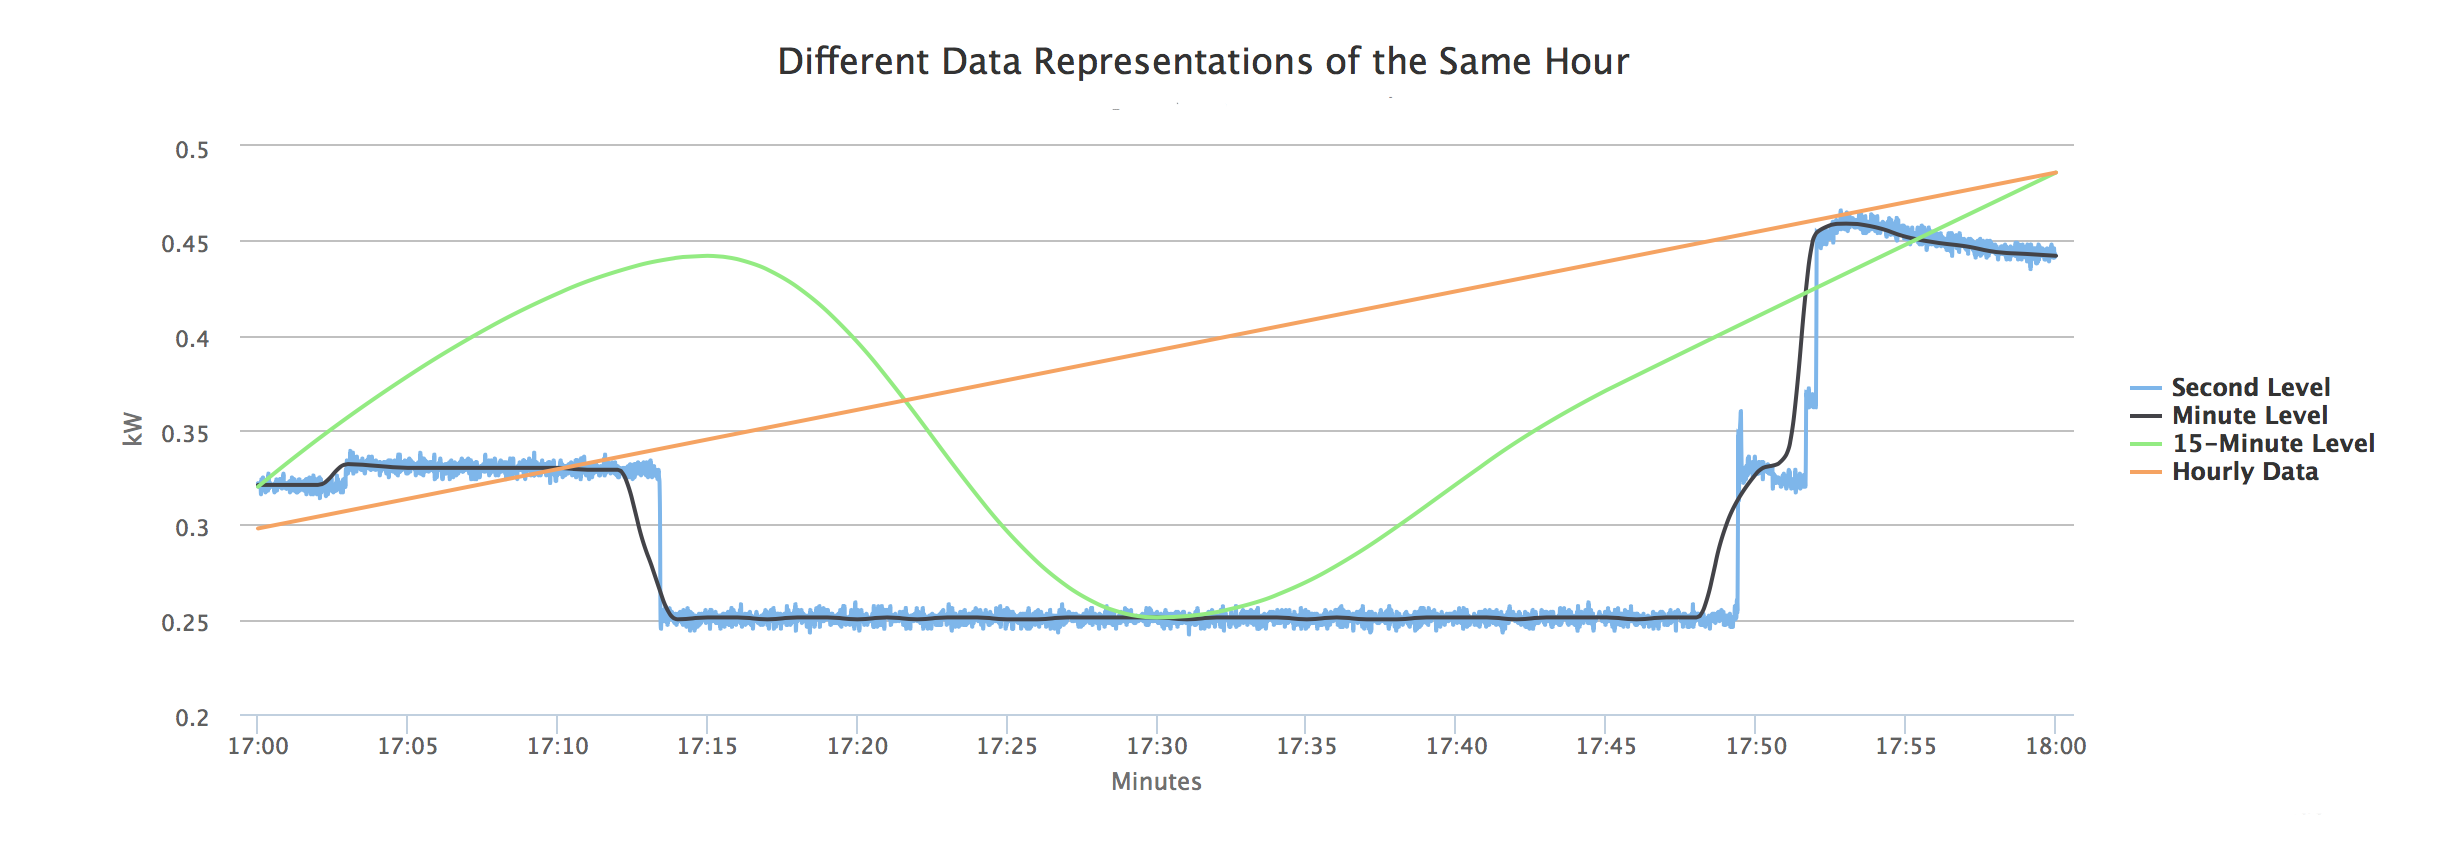
\includegraphics[scale=0.37]{./figures/hourlyexamplefixed.png}
	\caption{A figure to display the difference between low (that of hourly readings) to high resolution data. \protect\footnotemark}
	\label{fig:hourex}
\end{figure}
\footnotetext{Pecan Street Inc, 'Dataport', https://dataport.pecanstreet.org/, (accessed 10 June 2015)}

Energy disaggregation methods do have a long history in the engineering community, including some which have applied machine learning techniques — early algorithms \cite{hart} typically looked for “edges” in power signal to indicate whether a known device was turned on or off; later work focused on computing harmonics of steady-state power or current draw to determine more complex device signatures \cite{load}; recently, researchers have analyzed the transient noise of an electrical circuit that occurs when a device changes state \cite{patel}. However, these and most other studies we are aware of, were either conducted in artificial laboratory environments, contained a relatively small number of devices, trained and tested on the same set of devices in a house, and/or used custom hardware for very high frequency electrical monitoring with an algorithmic focus on “event detection” (detecting when different appliances were turned on and off) \cite{DDSC}.

\begin{figure}[H]
	\centering
	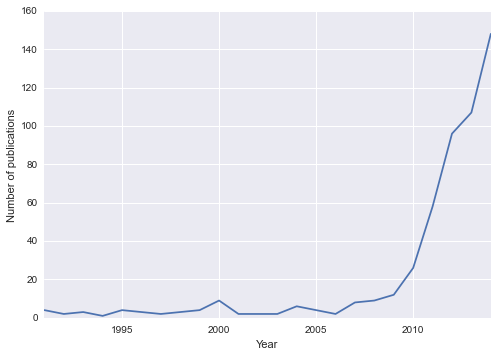
\includegraphics[scale=0.43]{./figures/growth}
	\caption{The number of publications related to NILM research. \protect\footnotemark}
	\label{fig:growth}
\end{figure}%
\footnotetext{Oliver Parson, \texttt{http://blog.oliverparson.co.uk/2015/03/overview-of-nilm-field.html}, 25 March 2015, (accessed 10 June 2015)}
Recent development within technology and the adoption of big data has influenced and researchers often refer to a recent explosion in the number of NILM publications. The figure \ref{fig:growth} shows the number of papers published per year, from which the upward trend since 2010 is clearly visible. This renewed interest is likely due to recent countrywide rollouts of smart meters. 

\begin{figure}[H]
	\label{fig:citations}
	\centering
	\begin{minipage}{.45\textwidth}
		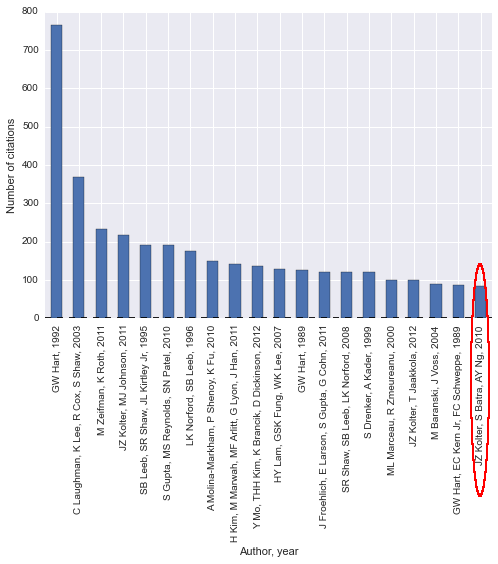
\includegraphics[scale=0.35]{./figures/citations_mod}
	\end{minipage}
	\begin{minipage}{.45\textwidth}
		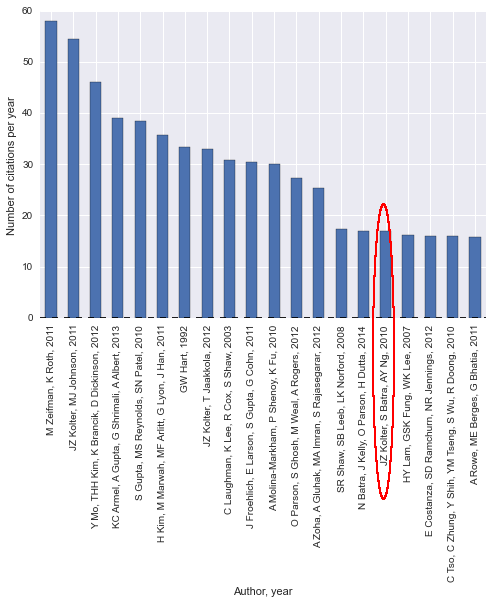
\includegraphics[scale=0.33]{./figures/citationsperyear_mod}
	\end{minipage}
	\caption{The figure shows citations of NILM related publications and highlights the paper by Kotler et. al \cite{DDSC}. The figure to the left shows number of citations overall, while the right figure show the number of citations for the year 2014. \protect\footnotemark}
\end{figure}

\footnotetext{Oliver Parson, \texttt{http://blog.oliverparson.co.uk/2015/03/overview-of-nilm-field.html}, 25 March 2015, (accessed 10 June 2015)}
Since older papers have had more time to accumulate citations, it's also interesting to look at citations per year to get a better idea of recent trends in the field, as shown by the graph on the right. Unlike before, there is no standout paper, with recent review papers and data set papers receiving the greatest citation velocity. One can see that the paper has not been the primary focus of research and is therefore interesting to look into. Besides these papers, a number of the remaining highly cited papers propose techniques based upon principled machine learning models. Most of the papers also focus on high-resolution data; in contrast, this thesis focuses on disaggregating electricity using low-resolution, hourly data of the type that is readily available via smart meters (but where most single-device “events” are not apparent); where we specifically look at temporal differences.

The method builds upon sparse coding methods and recent work in block-coordinate descent \cite{blondel,block2}. Specifically, we use a structured perceptron sparse coding algorithm presented in \cite{DDSC} using a coordinate descent approach to learn a model of each device’s power consumption over the specified time domains, week, two weeks and a month. While energy disaggregation can naturally be formulated as such a single-channel source separation problem, there is no previous application of these methods to the energy disaggregation task, until Kotler, Batra and Ng's algorithm \cite{DDSC}, presented in algorithm \ref{alg:ddsc}. Indeed, the most common application of such algorithm is audio signal separation, which typically has very high temporal resolution; thus, the low-resolution energy disaggregation task we consider here poses a new set of challenges for such methods, and existing approaches alone perform quite poorly. This thesis shows that the methods presented in \cite{DDSC} was cumbersome to implement and evaluate. The thesis also addressess the need for accurate energy consumption data, where the available dataset is far from being a good representation of the consumption inside a whole house. It also addresses that temporal differences have not affected the accuracy.

\subsection{Purpose}

The work described in this thesis was carried out at Greenely \protect\footnotemark. Greenely is a mobile application company based in Sweden, where a gamification model to educe a better energy consumption when providing consumers with their energy bills is being developed. Their solution is solely based on total energy consumption bills but would like to investigate a possible disaggregation for their costumers.

\footnotetext{Greenely, \texttt{http://greenely.com/about-us/}, 25 Feb 2015, (accessed 10 June 2015)}

The work has been to provide Greenely with steady insights of the energy disaggregation field as well as to implement Kotler et.al. models for a base model for energy disaggregation. The thesis aims to try to replicate their algorithm with using less data by using it on subsets of a larger dataset and therefore achieve reasonable disaggregation results. The performance results are presented and used for deciding whether or not to adopt the devised algorithm for their energy disaggregation.

\pagebreak[3]
\subsection{Thesis outline}
\label{sec:outline}
\begin{itemize}
	\item{Introduction}
	\begin{itemize}
		\item{\intOverview}
	\end{itemize}
	\item{Preliminaries}
	\begin{itemize}
		\item{}\preOverview
	\end{itemize}
	\item{Problem definition}
	\begin{itemize}
		\item{}\proOverview
	\end{itemize}
	\item{Fabrication}
	\begin{itemize} 
		\item{}\fabOverview
	\end{itemize}
	\item{Results}
	\begin{itemize}
		\item{}\resOverview
	\end{itemize}
	\item{Conclusions}
	\begin{itemize}
		\item{}\conOverview
	\end{itemize}
\end{itemize}

\newpage
%Preliminaries/Theory/Scientific Background/
\section{Preliminaries}
% Is there any useful theory? What are the methods used
% before for similar problems?
Throughout this paper, bold capital letters denote matrices (e.g., $\mathbf{X}$) and bold lower-case letters denote column vectors (e.g., $\mathbf{x}$). $\norm{\mathbf{X}}_2 =
(\mathbf{X}^T\mathbf{X})^{1/2}$ and $\norm{\mathbf{X}}_1 = \sum_i |\mathbf{x}_i|$
denote the $l_2$ and $l_1$ norms, respectively, with $T$ indicating the
matrix transpose. We also denote $\norm{\mathbf{X}}_F =
(\text{Tr}(\mathbf{X}^T\mathbf{X}))^{1/2}$ as the Frobenius norm, where
Tr indicate the trace of a matrix, i.e.,  $\text{Tr}(X)\equiv \sum_{i=1}^n \mathbf{x}_{ii}$.

This section contains the theory to implement a model such as the model presented in section \ref{sec:fab}. We first present a brief overview of the mathematical background behind Optimization, Machine Learning and Artificial Neural Networks (ANN) in sections \ref{sec:opt},\ref{sec:ml} and \ref{sec:ann} respectively. This theory leads up to all the necessary details involved with Sparse Coding, which is presented in \ref{sec:sc} with two examples in computer vision and speech recognition to give the reader a better understanding of the concept. We later present an underlying concept called Non-Negative Matrix-Factorization in section \ref{sec:nnsc} and the proof behind it. This technique is commonly used when dealing with tasks involving only positive values. 

%Lastly we present techniques for sparse approximations in section \ref{sec:regularization}.

\label{sec:theoretical}

\subsection{Optimization}
\label{sec:opt}
A problem that consists of finding the best solution from a set of feasible solutions. In mathematics and computer science, we refer this as a optimization problem. The standard form of a optimization problem is defined as

\begin{align*}
& \underbrace{\text{min}}_{x} \qquad f(x) \\
& \text{subject to} \quad g_i(x) \leq 0, \ i = 0,\dots,n
\end{align*}
where we define $f(x)$ as the objective function to be minimized with respect to $x$ and $g_i(x)$ as the $i$:th constraint. By convention, the standard form is to minimize the objective function, we can maximize by negating the expression above \cite{convex}.

\subsubsection{Cost function}

An objective function that is of standard form is often referred to as a cost or loss function that maps events or values of variables to some value that represents the "cost" involving that particular event. In classification, the cost is usually portrayed as "penalty" involving an incorrect classification. 

Supervised learning tasks, described in \ref{sec:ml}, such as regression or classification for parameter estimation can be formulated as a loss function over a training set. The goal is to find the models that represent the input well; and the loss function quantifies the amount of deviation of the prediction from the true values \cite{convex}.

\subsection{Machine Learning}
\label{sec:ml}
Machine learning can be considered a sub-field of computer science and statistics which can be described as the study of algorithms that can learn from data. Mostly Machine learning is employed on computational tasks where designing and programming explicit, rule-based algorithms is infeasible. The common applications include spam filtering, optical character recognition (OCR), search engines and computer vision. It also has ties to both artificial intelligence and optimization.

Machine learning tasks are typically classified into three broad categories, depending on the nature of the learning "signal" or "feedback" available to a learning system. One category is Supervised learning; where the computer is presented with example inputs and their desired outputs, given by the user, and the goal is to learn a general rule that maps inputs to outputs. The second category is Unsupervised learning, where no labels are given to the learning algorithm. This way the algorithm has to find its own structure in the input, this algorithm can be run to do stand-alone unsupervised learning (discover hidden patterns) or a means towards another type of end. Sparse Coding, which forms the basis of this thesis is a neural network model for unsupervised learning. Lastly we have reinforcement learning where a computer program interacts with a dynamic environment in which it must perform a certain goal (such as driving a vehicle), without a teacher explicitly telling it whether it has come close to its goal or not. Another example is learning to play a game by playing against an opponent \cite{ainorvig}.

A core objective of a learner is to generalize from its experience. Generalization in this context is the ability of a learning machine to perform accurately on new, unseen examples/tasks after having experienced a learning data set \cite{bishop, bengio}. The training examples usually come from some unknown probability distribution and the learner has to build a general model so as to produce sufficiently accurate predictions from incoming new examples. 

In machine learning one can simplify the inputs by mapping them into a lower-dimensional space through dimensionality reduction, described in section \ref{sec:dim}.

\subsubsection{Dimensionalty Reduction}
\label{sec:dim}

Representing an object as a vector of $n$ elements, we say that the vector is in $n$-dimensional space. Dimensionalty reduction refers to a process of representing the object of $n$-dimensional vector to an $m$-dimensional vector, where $m < n$. By refining the data in this way, we may lose information that might be valuable but we can represent it using less dimensions and in some cases we can even make a better prediction or analysis using this subspace. The common linear dimensionality reduction is called Principal Component Analysis (PCA), which find "internal axes" of a dataset, called components and sort by importance. It performs a linear mapping of the data to a lower-dimensional space in such a way that the variance of the data in the low-dimensional representation is maximized. The original space is not retained, i.e. we have lost some information but keep the most important variance to the space spanned by a few eigenvectors. The first $m$ components are then used as the new basis. Each of these components may be thought of as a high-level feature, describing data vectors better than original axes \cite{dr}.

Dimensionality reduction can be divided into feature selection and feature extraction. Feature selection approaches try to find a subset of the original variables, while feature extraction transforms the data in high-dimensional space to that of a fewer dimensional space. The data transformation may be linear, as in PCA, but many nonlinear dimensionality reduction techniques also exist \cite{samet}. 

A different approach to nonlinear dimensionality reduction is through the use of autoencoders, a special kind of feed-forward neural networks with a bottle-neck hidden layer, which is presented in-depth in section \ref{sec:autoencoders}.

\subsubsection{Deep Learning}
\label{sec:deeplearning}

A branch of machine learning based on algorithms that try to model high-level abstractions in data by using complex structures or multiple non-linear transformations is referred to deep learning \cite{deep, deep2}. Deep learning focuses on learning representations of data, where it has maybe come to replacing handcrafted features with efficient algorithms for unsupervised or semi-supervised feature learning and hierarchical feature extraction \cite{deep3}.

Some representation are based on interpreting information processsing in a nervous system inspired by advances in neuroscience, such as neural coding which attempts to define a relationship between the stimulus and the neuronal responses and the relationship among the electrical activity of the neurons in the brain \cite{nervous}, see section \ref{sec:scnn} for more information.



\subsection{Artificial Neural Networks}
\label{sec:ann}

In machine learning, a family of statistical learning algorithms called artificial neural networks (ANN) that were inspired by the work of McCulloch, Warren; Walter Pitts as early as 1943 to reflect a central nervous systems of animals \cite{1943}. Generally ANN is a network with connected nodes and edges that form a artificial "biological neural network" which compute values from inputs provided by the edges connected to the nodes, even though the relation between the model and the brain is debated to what degree it really represents the brain \cite{brain}. 

ANN models are essentially mathematical functions defining a function 
\begin{equation} 
f : X \rightarrow Y
\end{equation}

but sometimes models are also associated with a particular learning algorithm, like the perceptron presented in the section \ref{sec:perceptron} below. The learning output is obtained by connection weights, parameters and specific architecture by the learning algorithm. Two frameworks where ANN have made a great contribution is computer vision and speech recognition tasks, where rule-based programming have been unsuccessful at detecting patterns \cite{perceptron}. The connection between neural networks and Sparse Coding is explained in section \ref{sec:scnn}.

There are two main ways to "feed" the network with information. One being that of a feedforward neural network, the term “feedforward” indicates that the network has links that extend in only one direction. Except during training, there are no backward links in a feedforward network; all links proceed from input nodes toward output nodes. Eventually, despite the apprehensions of earlier workers, a powerful algorithm for apportioning error responsibility through a multi-layer network was formulated in the form of the backpropagation algorithm \cite{backpro}. The effects of error in the output nodes are propagated backward through the network after each training case. The essential idea of backpropagation is to combine a non-linear multi-layer perceptron-like system capable of making decisions with the objective error function of the Delta Rule \cite{backpro}.
% checked

\pagebreak
\subsubsection{Perceptron}
\label{sec:perceptron}
The basic concept of a single layer perceptron was introduced by Rosenblatt in 1958 \cite{perceptron}. It computes a single output by forming a linear combination of real-valued inputs and weights to possibly giving it through some non-linear function. This can be written as

\begin{equation} 
 y = \phi( \sum\limits_{i=1}^n a_i x_i + b ) = \phi( \mathbf{a}^T \mathbf{x}+ b )
\end{equation}

where  $\mathbf{a}$ denotes the vector of weights,  $ \mathbf{x}$ is the vector of inputs, $ b$ is the bias and $ \phi$ is the activation function. Usually in multilayer networks, the activation function is often chosen to be the logistic sigmoid $ 1 / (1 + e^{-x})$ or the hyperbolic tangent $ \tanh(x)$. They are convenient as they are close to linear near the origin, while they converge to a value when leaving the origin. This allows perceptron networks to model well both strongly and mildly nonlinear mappings \cite{nonlinear}. Perceptrons were a popular machine learning solution in the 1980s, but since the 1990s faced strong competition from the much simpler support vector machines \cite{svm}. More recently, there has been some renewed interest in backpropagation networks, such as perceptrons due to the successes of deep learning, see section \ref{sec:deeplearning} for more detail.

A typical perceptron layer network consists of source nodes forming the first layer. Following with one or more hidden layers, and an output layer of nodes, in the case where we have three or more layers it is usually called a multilayer perceptron (MLP). The input signal propagates through the network layer-by-layer. The signal-flow of such a network with one hidden layer can be seen in figure \ref{fig:autoencoder} in section \ref{sec:autoencoders}.

The computations performed by such a feedforward network with a single hidden layer with nonlinear activation functions and a linear output layer can be written mathematically as

\begin{equation}
\mathbf{y}= \mathbf{f}(\mathbf{x}) = \mathbf{B}\boldsymbol{\phi}( \mathbf{A}\mathbf{x}+ \mathbf{a} ) + \mathbf{b}
\label{eq:nonlinear}
\end{equation}

where  $\mathbf{x}$ is a vector of inputs and  $\mathbf{y}$ a vector of outputs.  $ \mathbf{A}$ is the matrix of weights of the first layer,  $ \mathbf{a}$ is the bias vector of the first layer.  $ \mathbf{B}$ and  $ \mathbf{b}$ are, respectively, the weight matrix and the bias vector of the second layer. 

MLP networks are typically used in supervised learning problems. Here the training set of input-output is pairs and the network must learn to model the dependency between them. The training here means adapting all the weights and biases ( $ \mathbf{A},
\mathbf{B}, \mathbf{a}$ and  $ \mathbf{b}$ in equation \ref{eq:nonlinear} to their optimal values for the given pairs  $ (\mathbf{x}(t), \mathbf{y}(t))$. The criterion to be optimised is typically the squared reconstruction error.
%to read more on regression see section \ref{sec:regularization}

\begin{equation}
\label{eq:error}
\sum_t \vert\vert\mathbf{f}(\mathbf{x}(t)) - \mathbf{y}(t)\vert\vert^2.
\end{equation}

By setting the same values for the inputs as well as the outputs of the network, MLP networks can be used for unsupervised learning. The values of the hidden neurons extract the sources, this approach however is rather computationally intensive. \cite{hidden}

\subsubsection{Autoencoder}
\label{sec:autoencoders}

Autoencoder is a simple 3-layer neural network where output units (Layer $L_3$) are directly connected back to input units (Layer $L_1$). E.g. in a network presented in the figure below:

\begin{figure}[H]
	\centering
	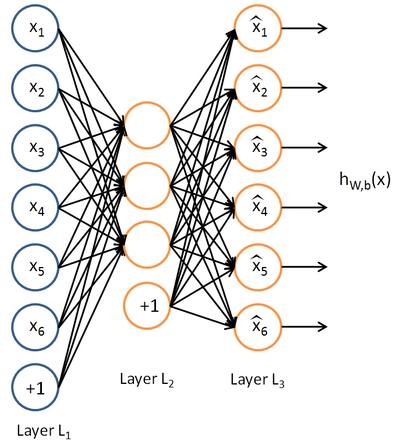
\includegraphics[scale=0.3]{./figures/autoencoder}
	\caption[Caption for LOF]{As a concrete example, suppose the inputs $x$ are the pixel intensity values from a $10 \times 10$ image (100 pixels) so  $n=100$, and there are $s_2=50$ hidden units in layer $L_2$.	\protect\footnotemark}
	\label{fig:autoencoder}
\end{figure}
\footnotetext{Stanford, \texttt{http://ufldl.stanford.edu/wiki/index.php/Autoencoders\_and\_Sparsity},7 April 2013, (accesed 10 July 2015)}
Typically in an autoencoder, the number of hidden units are much less than number of input and output. As a result, it first compresses (encodes) the input vector to "fit" in a smaller representation, and then tries to reconstruct (decode) it back. Here is where Sparse Coding can be said to be an extension of autoencoders with the constraint that the hidden layer must mostly be unused nodes (sparse), for more information on their similarities see the end of section \ref{sec:sc}. Autoencoders simple form can be written as
%\[ D(d(e(x;\theta^r); \theta^d), x) \]

\begin{equation}
\label{eq:auto}
\norm{\mathbf{A}\sigma(\mathbf{A}^T \mathbf{x}) - \mathbf{x}}^2
\end{equation}

where $\sigma$ is a nonlinear function such as the logistic sigmoid, and $\mathbf{A}$ is the activation density of the nodes. Once a deep network is pretrained, input vectors are transformed to a better representation. \cite{autoencoder2}

\subsubsection{Sparse Coding and the connection to Neural Networks}
\label{sec:scnn}

Information retrieved is presented in the brain by the pattern of activations of the nerual connections formed, which we say form a neural code. This defines the pattern at which the neural activity corresponds to each presented information. 
% - rewrite
One property of the neural code is the fraction at which the neurons are active at any time. If a set of $N$ neurons, which can be active in the region $\in [0,1/2]$ corresponding to low activity to strong activity, the expected value of this fraction is the density of the code. If the average fraction is above 1/2 we can replace each active neuron with an inactive one causing the fraction activity to get below 1/2 without loss of information and vice versa. Sparse coding is a neural code, which is of a relatively small set of neurons but with strong activity. For each set of information, a different subset is triggered of all available neurons.\cite{scprimate}

\subsubsection{Local Codes}
Low activity of neurons are local codes, where an item is represented by a small set of neurons or a separate neuron, this way one can ensure that there is no overlap between the representations of two items. To understand this we make an analogy that envolves the characters on a computer keyboard, where each key encodes a single character. This scheme has the advantage that it is simple and is also easy to decode, due to local codes only representing a finite number of combinations. More generalization is essential and a widely observed behavior. \cite{mclaren}

\subsubsection{Dense Distributed Codes}

% - rewrite
The opposite of local codes are dense codes, where the average activity ratio is $\geq 0.5$, the item is represented by activities of all the neurons, which implies a representational capacity of $2^N$. Given the billions of neurons in a human brain, $2^N$, as the number of neurons the representational capacity of a dense code in the brain is immense, therefore its greatest feature is dealing with redundancy. Dense codes limit the number of memories that can be stored in an associative memory by simple learning rules. On the contrast, dense codes may facilitate good generalization performance and high redundancy.

\subsubsection{Sparse Codes}
% - rewrite

These neural codes come to a favorable compromise between dense and local codes by having a small average activity ratio, called sparse codes \cite{scprimate}. We can redeem the capacity of local codes by a modest fraction of active units per pattern, thus interference by items represented simultaneously will be less likely as capacity grows exponentially with average activity ratio. It is more likely that a single layer network with a sparse representation as input can learn to generate a target output \cite{willshaw}. Due to linear discriminant functions being able to map higher proportions, see Perceptrons for linear separability in section \ref{sec:perceptron}. Single layer networks for learning is therefore simpler, faster and substantially more plausible as a way of a biological implementation in the brain, as the redundancy for fault tolerance can be chosen by controlling the sparseness.

For learning various tasks a neural code can therefore contain codewords of varying sparseness. This implies that we want to maximize sparseness while having a high representational capacity. One plausible way would be to assign sparse codes for items of high probability while having distributed codes for lower probability items.
A code with a given average sparseness can contain codewords of varying sparseness. If the goal is to maximize sparseness while keeping representational capacity high, a sensible strategy is to assign sparse codewords to high probability items and more distributed codewords to lower probability items. However, if we would only store identities of active units, the code would have short average discription length \cite{cover}. Some perceptual learning could be explained by prediction of the sparseness of the encoded items with high probability.

Below is an example where the input signal is an image, the basis vectors represent the sparse coding method. In the example below we present an explicit visualization of the sparse coding. 

\begin{ex}{}
\label{ex:scimage}
An image reconstruction usage of sparse coding. The basis vectors are visualized in Figure \ref{fig:basex}, which have been trained from natural images. The basis vectors are then used to represent different parts of a picture using the activation matrix.

\begin{figure}[H]
\centering
        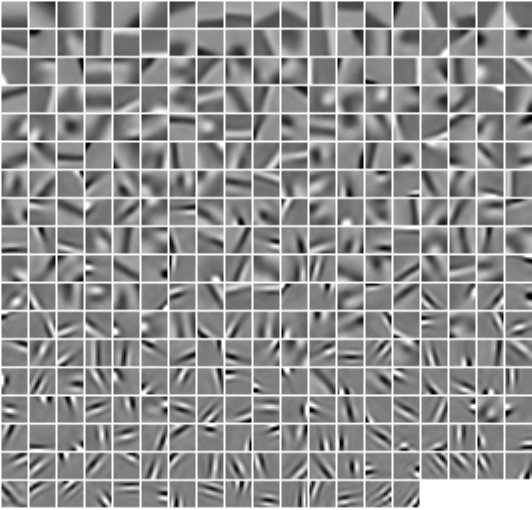
\includegraphics[scale=0.20]{./figures/basisexample.jpg}
        \caption{Sparse basis functions learned from images.}
        \label{fig:basex}   
\end{figure}

These basis vectors are used with activations to represent an image. The activation matrix is best represented in the figure below, where a part of an image uses the activated vectors (non-black) to represent the corresponding image.

\begin{figure}[H]
\centering
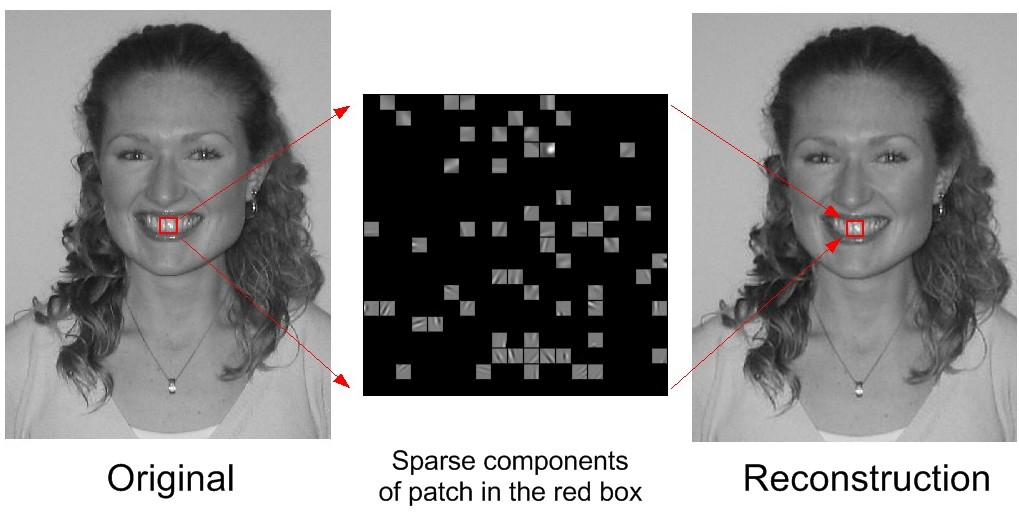
\includegraphics[scale=0.30]{./figures/Sparsejen_black_v2.jpg}
\caption{An image, encoded with the basis functions from figure \ref{fig:basex} and reconstructed in the right plot using certain subsets of activations and basis functions for each patch. The red square represents a patch where we have encoded the activations for some basis functions, shown as the middle plot, to reconstruct the patch of the decoded image to the right. Notice, among the entire set of basis functions, only a fair amount is used and the rest is black indicated that they are not being used, i.e. we have a "sparse" representation of the image. \protect\footnotemark
}
\label{fig:recex}
\end{figure}

\end{ex}
\footnotetext{Peter Foldiak and Dominik Endres ,Scholarpedia, \texttt{http://www.scholarpedia.org/article/Sparse\_coding}, 2008, (accessed 10 June 2015)}
\newpage

\subsubsection{Sparse Coding}

\label{sec:sc}
Sparse Coding is similar to Principal Component Analysis (PCA) in that we want to find a small number of basis functions to represent an input signal as a linear combination presented in equation \ref{eq:lincomb} but with a constraint that the learned basis functions need to be sparse and of a higher dimension than the input data. Here we present the general theory behind Sparse Coding and an example used for signal processing in example \ref{ex:sc} \cite{olshausen}.

\begin{equation}
\mathbf{x} \approx \mathbf{BA}
\label{eq:lincomb}
\end{equation}

Consider a linear system of equations $\mathbf{x} = \sum_{i=1}^ka_i \phi_i$, the vector coefficients $a_i$ are no longer uniquely determined by the input vector $\mathbf{x}$, where $\sum_{i=1}^ka_i = \mathbf{B}$ is an
underdetermined $m\times p$ matrix $(m \ll p)$. $\mathbf{B}$, is called the dictionary or sometimes design matrix. The problem is to estimate the signal $\alpha$, subject to the
constraint that it is sparse. The underlying motivation for sparse
decomposition problems is that even though the observed values are in
high-dimensional ($m$) space, the actual signal is organized in some
lower-dimensional subspace $(k \ll m)$. This implies that $\mathbf{x}$ can be decomposed as a linear combination of only a few $m \times 1$ vectors in $\mathbf{B}$, called atoms \cite{sc}.

Regular PCA allows us to learn a complete set of basis vector while the Sparse Coding wishes to learn an \textbf{over-complete}
basis to recognize patterns and structures inherent in the input data.
Although we now can recognize patterns in the data, we have coefficients of the columns
$\alpha_i$ that are no longer uniquely determined by the input vector
$\mathbf{x} \in \mathbb{R}^2$. This is why we introduce a criterion called
\textbf{sparsity} to resolve the degeneracy introduced by
over-completeness, where sparsity is defined as having few non-zero
components. The definition of the sparse coding cost function on a set of $m$
input vectors is presented in equation \ref{eq:sccost}. In artificial
neural networks, the cost function represents a function to return a number representing how well the neural network performed to map training examples to correct output \cite{olshausen}.

%\begin{equation}
%\mathbf{x} = \mathbf{BA}
%\label{eq:lincomb}
%\end{equation}
%
%Consider a linear system of equations $\mathbf{x} = \mathbf{BA}$, where $\mathbf{B}$ is an
%under-determined $m\times p$ matrix $(m \ll p)$. $\mathbf{B}$, is called the dictionary or the design matrix. The problem is to estimate the signal $\mathbf{A}$, subject to the
%constraint that it is sparse. The underlying motivation for sparse
%decomposition problems is that even though the observed values are in
%high-dimensional ($m$) space, the actual signal is organized in some
%lower-dimensional subspace $(k \ll m)$. This implies that $\mathbf{x}$ can be decomposed as a linear combination of only a few $m \times 1$ vectors in $\mathbf{B}$, called atoms. 
%
%Regular PCA allow us to learn a complete set of basis vector while the Sparse Coding wish to learn a \textbf{over-complete}
%basis to recognize patterns and structures inherent in the input data.
%Although we now can recognize patterns in the data, we have coefficients of the columns
%$\mathbf{B}^(j)$ that are no longer uniquely determined by the input vector
%$\mathbf{x} \in \mathbb{R}^2$. This is why we introduce a criterion called
%\textbf{sparsity} to resolve the degeneracy introduced by
%over-completeness, where sparsity is defined as having few non-zero
%components. The definition of the sparse coding cost function on a set of $m$
%input vectors is presented in equation \ref{eq:sccost}. In artificial
%neural networks, the cost function represents a function to return a number representing how well the neural network performed to map training examples to correct output.

\begin{equation}
\min_{a_i^{(j)},\phi_i}\sum_{j=1}^m
\ \underbrace{\norm{\mathbf{x}^{(j)}-\sum_{i=1}^ka_i^{(j)}\phi_i}^2}_{\text{reconstruction term}}+\underbrace{\lambda \sum_{i=1}^k
S(a_i)^{(j)}}_{\text{sparsity penalty}}
\label{eq:sccost}
\end{equation}

where $S(a_i^{(j)})$ is a sparsity cost function which penalize $a_i$ for being far from zero.
%and $\norm{\mathbf{x}^{(j)}-\sum_{i=1}^ka_i^{(j)}\phi_i}^2 = \sum_{ij} [\mathbf{x}_{ij}-(a \phi)_{ij} ]^2$.
The first term in equation \ref{eq:sccost} is a reconstruction term that forces the algorithm to provide a good representation of $\mathbf{x}$ and the second as a sparsity penalty which force the representation to be sparse, while $\lambda$ is a scale to determine the relative importance between the two contributions. Note that if we are given $S(a_i^{(j)})$, estimation of $\phi_i$ is easy via least squares. In the beginning, we do not have $S(a_i^{(j)})$ however. Yet, many algorithms exist that can solve the objective above with respect to $S(a_i^{(j)})$. 

%Actually, this is how we do inference: we need to solve an optimisation problem if we want to know the h belonging to an unseen $\mathbf{x}$.
% timo banned it

The most direct approach to determine sparsity is through the "$L_0$" norm $S(a_i) = \mathbf{1}(|a_i| > 0 )$, which is non-differentiable and difficult to optimize. The more common choices for sparsity cost penalty $S(a_i)$ are the $L_1$, $S(a_i) = |a_i|_1$ and the log penalty $S(a_i)=\log(1+a^2_i)$. To prevent empirical scaling of $a_i$ and $\phi_i$ to make the sparsity penalty arbitrarily small, we constrain $\norm{\phi}^2$ to be less than some constant $C$. Including the constraint demand we get the full sparse coding cost function \cite{olshausen}

\begin{align}
\begin{split}
\min_{a_i^{(j)},\phi_i} \quad & \sum_{j=1}^m
\norm{\mathbf{x}^{(j)}-\sum_{i=1}^ka_i^{(j)}\phi_i}^2+\lambda \sum_{i=1}^kS(a_i)^{(j)}
\\
\text{subject to} & \quad \norm{\phi_i}^2 \leq C, \forall \ i = 1,\dots,k
\end{split}
\end{align}

Below we present another example of sparse coding but used in a context of signal processing of a one dimensional signal.
\begin{ex}{}
\label{ex:sc}
Say, we have an infinite $1-D$ time-series signal. We can represent this signal in the Fourier domain, where we get a few coefficients representing the whole signal in a different domain.
\begin{equation*}
\mathbf{x} = \sum_{i=1}^k a_i \phi_i \approx \mathbf{x}'
\end{equation*}

We want to find these few coefficients ($a_i$,the basis) of an input signal in the alternative domain and reconstruct your signal with these few coefficients. Once we have found the coefficients, we determine how close is the reconstructed signal to our original input signal by the error. That is to minimize our representation: $|\mathbf{x}- \mathbf{x}'|$.

The least number of basis functions of the input signal that minimize the above error, is the best basis representation of our input signal. We then could use the $L_2$ norm for the error, which is what we are most familiar with and it computes the Euclidean, square difference, between basis functions. Basically, $L_0$ norm looks like a Dirac Delta Function, $L_1$ norm looks like a diamond and $L_2$ norm looks like a circle and are the other types of norms which can be used in this context.

\end{ex}

To end this section we would like to review the difference between Sparse Coding, Autoencoders and Sparse-PCA, as it is somewhat missleading at times.

\begin{itemize}
	\item{Autoencoders do not encourage sparsity in their general form.}
	\item{An autoencoder uses a model for finding the codes, while sparse coding does so by means of optimisation.}
\end{itemize}

Note that Sparse Coding, looks almost the same as Autoencoder as in equation \ref{eq:auto} in section \ref{sec:autoencoders} Autoencoders, once we set $\mathbf{B}=\sigma (\mathbf{A}^T\mathbf{x})$. For natural image data, regularized autoencoders and sparse coding tend to yield very similar $\mathbf{B}$. However, auto encoders are much more efficient and are easily generalized to much more complicated models. E.g. the decoder can be highly nonlinear, e.g. a deep neural network. Therefore, Sparse coding can be seen as a modification of the sparse autoencoder method in which we try to learn the set of features for some data "directly".

In Sparse-PCA one also wants to represent a collection of vectors as a linear combination of basis vectors (a.k.a. principal components). Here the focus, as in traditional PCA, is on choosing a small $n \ll M$ number of basis vectors that together "explain as much variance" as possible, i.e. represent the original data as well as possible. And the sparsity is enforced not on the mapping bases $\rightarrow$data, but on the mapping data$\rightarrow$bases, because the idea is to have PCs that are linear combinations of only small subsets of original features/vectors (to ease the interpretation), as explained in Zou, Hastie, and Tibshirani, 2006 \cite{zou}.

\subsubsection{Non-Negative Sparse Coding}

\label{sec:nnsc}
In standard Sparse Coding, described above, the data is described as a combination of elementary features involving both additive and subtractive interactions. The fact that features can ‘cancel each other out’ using subtraction is contrary to the intuitive notion of combining parts to form a whole \cite{hoyer}. Arguments for non-negative representations come from biological modeling, where such constraints are related to the non-negativity of neural firing rates. These non-negative representations assume that the input data $\mathbf{X}$, the basis $\mathbf{B}$, and the hidden components $\mathbf{A}$ are all non-negative. Since energy consumption is an inherently non-negative quantity, this representation is beneficial is reasonable for modeling energy usage. \\
Non-negative matrix factorization (NMF) can be performed by the minimization of the following objective function:

\begin{equation}
\label{eq:nmf}
C ( \mathbf{A,B} ) = \frac{1}{2} \norm{ \mathbf{X} - \mathbf{BA} }^2
\end{equation}

Here Hoyer \cite{hoyer} take $ \norm{ \mathbf{X} - \mathbf{BA} }^2 = \sum_{ij} [ \mathbf{X}_{ij} - \mathbf{BA}_{ij} ]^2$. Denoting a general matrix norm by

\begin{equation}
\| A \|_{p,q}  =  \left[\sum_{j=1}^n \left( \sum_{i=1}^m |a_{ij}|^p \right)^{q/p}\right]^{1/q}
\end{equation}

Using $p=2,q = 2$ we get the Frobenius norm and we conclude that equation \ref{eq:nmf} is using the Frobenius norm, this is an insurance for later use in the Discriminative Disaggregation via Sparse Coding model \ref{alg:ddsc}.
\[ \|A\|_F^2 =\left(\sqrt{\sum_{i=1}^m\sum_{j=1}^n |a_{ij}|^2}\right)^2 = \sum_{i,j}[a_{ij}]^2\]


\textbf{Definition 1.} Non-negative sparse coding (NNSC) of a non-negative data matrix $\mathbf{X}$ (i.e. $\forall \ i,j \ : \ X_{ij} \geq 0$) is given by the minimization of
\begin{equation}
\label{eq:nnsc}
C ( \mathbf{A,B} ) = \frac{1}{2} \norm{ \mathbf{X} - \mathbf{BA} }^2 + \lambda \sum_{ij} \mathbf{A}_{ij}
\end{equation}
subject under the constraints $\forall \ i,j \ : \ B_{ij} \geq 0, \ A_{ij} \geq 0$ and $\forall \ i \ : \ \| \mathbf{B}_i \| = 1$, where $\mathbf{B}_i$ denotes the i:th column of $\mathbf{B}$. It is also assumed that the constant $\lambda \geq 0$. 
~\\

\pagebreak
\textbf{Theorem 1.} The equation \ref{eq:nmf} is non-increasing under the update rule:
\begin{equation}
\label{eq:update}
\mathbf{A}^{t+1}=\mathbf{A}^t.*(\mathbf{B}^T\mathbf{X})./(\mathbf{B}^T\mathbf{B}\mathbf{A}^t+\lambda)
\end{equation}
where $.*$ and $./$ denote element-wise multiplication and division (respectively), and the addition of the scalar $\lambda$ is done to every element of the matrix  $\mathbf{B}^T\mathbf{B}\mathbf{A}^t$.
~\\

The proof is seen below in \ref{proof:noninc}. As each element of $\mathbf{A}$ is updated by simply multiplying with some non-negative factor, it is guaranteed that the elements of $\mathbf{A}$ stay non-negative under this update rule. As long as the initial values of $\mathbf{A}$ are all chosen strictly positive, iteration of this update rule is in practice guaranteed to reach the global minimum to any required precision.

\begin{proof2}{Proof of Theorem 1}
To prove Theorem 1, first note that the equation \ref{eq:nnsc} in definition 1 is separable in the columns of $\mathbf{A}$ so that each column can be optimized without considering the others. We may thus consider the problem for the case of a single column, denoted s. The corresponding column of $\mathbf{X}$ is denoted $x$, giving the objective
\begin{equation}
F(\mathbf{a}) = \frac{1}{2}\norm{\mathbf{X}-\mathbf{B}\mathbf{a}}^2 + \lambda \sum_i a_i
\end{equation}
We need an iliary function $G(\mathbf{a},\mathbf{a}^t)$ with the properties that $G(\mathbf{a},\mathbf{a}) = F(\mathbf{a})$ and $G(\mathbf{a},\mathbf{a}^t) \geq F(\mathbf{a})$. We will then show that the multiplicative update rule corresponds to setting, at each iteration, the new state vector to the values that minimize the auxiliary function:
\begin{equation}
\mathbf{a}^{t+1} = \arg\!\min_{a} G(\mathbf{a},\mathbf{a}^t).
\end{equation}
This is guaranteed not to increase the objective function $F$, as
\begin{equation}
\label{eq:proof}
F(\mathbf{a}^{t+1}) \leq G(\mathbf{a}^{t+1},\mathbf{a}^t) \leq G(\mathbf{a}^t,\mathbf{a}^t) = F(\mathbf{a}^t).
\end{equation}
We define the function $G$ as
\begin{equation}
G(\mathbf{a},\mathbf{a}^t) = F(\mathbf{a}^t) + (\mathbf{a}-\mathbf{a}^t)^T \nabla F(\mathbf{a}^t) + \frac{1}{2} (\mathbf{a}-\mathbf{a}^t)^T\mathbf{K}(\mathbf{a}^t)(\mathbf{a}-\mathbf{a}^t)
\end{equation}
where the diagonal matrix $\mathbf{K}(\mathbf{a}^t)$ is defined by elementwise division as
\begin{equation}
K_{ij}(\mathbf{a}^t) = \delta_{ij}\frac{(\mathbf{B}^T\mathbf{B}\mathbf{a}^t)_i+\lambda}{\mathbf{a}^t_i},
\end{equation}
where $i$ denotes the $i$:th column. Inserting $\mathbf{a}$ in function $G$ we get the result from equation \ref{eq:proof}, $G(\mathbf{a},\mathbf{a}) = F(\mathbf{a})$. Writing out
\begin{equation}
F(\mathbf{a}) = F(\mathbf{a}^t) + (\mathbf{a}-\mathbf{a}^t)^T \nabla F(\mathbf{a}^t)+\frac{1}{2}(\mathbf{a}-\mathbf{a}^t)^T(\mathbf{B}^T\mathbf{B})(\mathbf{a}-\mathbf{a}^t),
\end{equation}
we see that the second property, $G(\mathbf{a},\mathbf{a}') \geq F(\mathbf{a}),$ is satisfied if
\begin{equation}
0 \leq (\mathbf{a}-\mathbf{a}^t)^T[\mathbf{K}(\mathbf{a}^t) - \mathbf{B}^T\mathbf{B}](\mathbf{a}-\mathbf{a}^t).
\end{equation}
Hoyer proved this positive semidefiniteness for the case of $\lambda \geq 0$ \cite{hoyer}. He concludes that as a non-negative diagonal matrix is positive semidefinite, and the sum of two positive semidefinite matrices is also positive semidefinite, the proof for $\lambda = 0$, in his paper also holds for $\lambda \geq 0$.
It remains to be shown that the update rule in equation \ref{eq:update} selects the minimum of $G$. This minimum is easily found by taking the gradient and equating it to zero:
\begin{equation}
\nabla_\mathbf{a} G(\mathbf{a},\mathbf{a}) = \mathbf{B}^T(\mathbf{B}\mathbf{a}^t-\mathbf{x}) + \lambda\mathbf{c} + \mathbf{K}(\mathbf{s}^t)(\mathbf{a}-\mathbf{a}^t)=0,
\end{equation}
where $\mathbf{c}$ is a vector with all ones. Solving for $\mathbf{a}$, this gives
\begin{align}
\mathbf{a} & = \mathbf{a}^t - \mathbf{K}^{-1}(\mathbf{a}^t)(\mathbf{B}^t\mathbf{B}\mathbf{a}^t-\mathbf{B}^T\mathbf{x}+\lambda \mathbf{c}) \\
& = \mathbf{a}^t-(\mathbf{a}^t./(\mathbf{B}^T\mathbf{B}\mathbf{a}^t+\lambda\mathbf{c})).* (\mathbf{B}^T\mathbf{B}\mathbf{a}^t - \mathbf{B}^T\mathbf{x}+\lambda \mathbf{c}) \\
& = \mathbf{a}^t.\times (\mathbf{B}^T\mathbf{x}./(\mathbf{B}^T\mathbf{B}\mathbf{a}^t+\lambda\mathbf{c}))
\end{align}
which is the desired update rule \ref{eq:update}.
\label{proof:noninc}
\end{proof2}


%\subsubsection{Tranformation Algorithms and variations for sparse approximation}
%%
%\label{sec:regularization}
%\subsubsection{Ridge Regression}
%
%A famous method of regularization called Tikhonov regularization, in statistics this method is known as ridge regression, an algorithm for non-linear least-squares problems. When x is non-existent, we call it an ill-posed problem such as below
%
%\begin{equation}
%A\mathbf{x}=\mathbf{b},
%\end{equation}
%
%a standard approach to the problem is ordinary least squares, which often leads to an underdetermined system of equations. Real-world problems often operate as a low-pass filter, meaning that the direction of the mapping where $A$ maps $\mathbf{x}$ to $\mathbf{b}$. By the inverse-mapping, we operate as a high-pass filter, which is often the case in mathematical formulations, it has an undesirable tendency of amplifying noise. \cite{ill-posed} Ordinary least squares (OLS) nullifies every element of the reconstructed elements of $\mathbf{x}$, that is in the null-space of $A$. The ridge regression uses the $l_2$-norm as a means of regression to the residuals and can be mathematically written as the following formulation
%\begin{equation}
%\label{eq:ridge}
%\beta^{ridge} = \arg \! \operatorname*{\min}_\beta \sum_{i=1}^n (\mathbf{y}_i - ( \beta_0 + \beta^T \mathbf{x}_i))^2 + \lambda \norm{\beta}^2_2
%\end{equation}
%There are other techniques which are based on the assumption that the $l_2$-norm does not capture the features to the respective dimensions and therefore "LASSO" has been used as a means of using the $l_1$-norm instead.
%
%\subsubsection{LASSO}
%
%"LASSO" In the context of regression and statistics, is fittingly being used as a metaphor of $L_1$ constraint applied to linear model. Coincidently, LASSO is also the initials for Least Absolute Shrinkage and Selection Operator. LASSO minimizes the residual sum of squares subject to the sum of the absolute value of the coefficients being less than a constant. LASSO not only helps to improve the prediction accuracy when dealing with multicolinearity data, but also carries several nice properties such as interpretability and numerical stability. Because of the nature of this constraint it tends to produce some coefficients that are exactly 0 and hence gives interpretable models \cite{lasso}. In a Bayesian context, this is equivalent to placing a zero-mean Laplace prior distribution on the parameter vector \cite{bayes_lasso}. The optimization problem may be solved using quadratic programming or more general convex optimization methods. The formulation of LASSO regression can mathematically be written as
%
%\begin{equation}
%\label{eq:lasso}
%\beta^{lasso} = \arg \! \operatorname*{\min}_\beta \sum_{i=1}^n (\mathbf{y}_i - ( \beta_0 + \beta^T \mathbf{x}_i))^2 + \lambda \norm{\beta}_1
%\end{equation}
%
%The difference between LASSO and ridge regression is that the penalty is increased and all parameters remain non-zero while still being reduced, using ridge regression. While increasing the penalty using LASSO will cause more and more of the parameters to be driven to zero. This makes LASSO an advantage for practical and model evaluation reasoning as we have to deal with less parameters to the model. As a result, LASSO selects more relevant features and discards the others, whereas ridge regression never fully discards any features. \cite{bayes_lasso}
%
%\subsubsection{Gradient Descent}
%
%The gradient descent method gives a way to find a local minimum of a given general function. We initialize the algorithm by a guess to the solution and compute the gradient for the function at the initial point. Next, we start the process of stepping through the negative direction of the gradient and repeat the process until the algorithm has converged at which the gradient is zero or until we reach a point at which we believe that there is no local minimum. The algorithm is called a first-order algorithm as it only takes the first derivative of the function into account.
%
%Here we will walk through the process of a gradient descent algorithm for finding the solution to the minimum of some function $f(x)$. Initializing with some initial value $x_0$ for $x$, we can change its value proportional to the dimension of x: with only one dimension; we can make it higher or lower. The best direction at $x_0$ to minimize $f$, we take the gradient $\nabla f$ along every dimension of $x$. Intuitively, the gradient will give the curve at that which $x$ will point to an increase in the function. Therefore we change $x$ in the opposite direction to lower the function value:
%\begin{equation}
%x_{k+1} = x_k - \lambda \nabla f(x_k)
%\end{equation}
%where $\lambda$ represents the stepsize in the discretization of the function we represent. This can be a fixed value or change depending on which implementation one decides to chose. Often $\lambda>0$ is a small number that forces the algorithm to make small jumps, even for the most minimal $\lambda$ it has been shown to converge to a minimum. As a result, the algorithm will be stable and its optimal value depends on the function, given stable conditions (and a certain choice of $\lambda$), it is guaranteed that $f(x_{k+1}) \leq f(x_k)$ \cite{gradient}.
%
%\subsubsection{Coordinate Descent}
%
%Instead of relying on the gradient of a function, one approach called the coordinate descent can minimize a function by minimizing it along one direction at a time. By the given regression model we can minimize the function $f(x)$.
%\begin{equation}
%y = X \theta,
%\end{equation}
% the function to minimise for a least squares regression is 
% \begin{equation}
% f(\theta) = | y- X \theta |^2.
% \end{equation}
% Minimising over $\theta$ is achieved by 
% \begin{equation}
% 0 = X_{i}^\top (X \theta - y) = X_{i}^\top (X_i \theta_i + X_{-i} \theta_{-i} -y).
% \end{equation}
% So the next step in the coordinate descent update is
% \begin{equation}
% \theta_{i} = \frac{X_{i}^\top(y- X_{-i}\theta_{-i})}{X_{i}^\top X_{i}}.
% \end{equation}
%Regardless the learning rate of the gradient descent procedure (which could indeed speed up convergence), the comparison between the two is fair at least in terms of complexity.
%Coordinate descent needs to perform $O(n)$ operations for each coordinate update (n operations to compute residuals $r = (y- X_{-i}\theta_{-i})$ and n to compute $X_{i}^\top r$ . Each cycle of this type is performed p times, where p is the number of covariates.
%Gradient descent performs the same number of operations $O(np)$.
%

% sparse coding, Discriminative vs Generative, Discriminative Disaggregation Sparse Coding, Non-Negative Sparse Coding
\newpage
\section{Problem Definition}
%• Problem definition: What is demanded from the solution? What is the aim of the study?
%Useful simplifications?
%• Problem definition: What is demanded from the solution? What is the aim of the study?
%Useful simplifications?
In this section we describe what is required of the solution and what this thesis aims at achieving as well as some useful simplifications made for this thesis.


Kotler et. al. \cite{DDSC} train the DDSC algorithm with weeks sampled across two years of data as to generalize the training. This thesis aims at reimplementing the algorithm and investigating the possibility of training with less data but taking the advantage of the temporal correlation between years as to further extend the algorithm by pre-processing the data better, by training the algorithm for the same timeperiod across two years instead of randomly.

\subsection{Solution}
%• Solution/Design: How is it to be done? Will it give the expected performance? What
%limitations can be foreseen from theory?

\begin{enumerate}
	\item{Retrieve similar data}
	\item{Pre-process}
	\item{Implementation}
	\item{Tweak algorithm using temporal difference}
\end{enumerate}

The first problem to address is to retrieve valuable and similar data mostly found via githubs \href{https://github.com/caesar0301/awesome-public-datasets}{Awesome-public-datasets} \cite{awesome}. Once the data has been decided on we pre-process and implement the algorithm, where the algorithm itself could pose a challenge as there is no explicit formulation stated in the paper \cite{DDSC}, nor any source code available. This thesis aims at reproducing the results, by focusing on exploiting the data at hand. The method relies substansually on the data, which could prove to produce very different results. The implementation is limited by the amount of computational power that is available as it run by standard student-laptop. This is reflected on the choice of training set and as well as the choice of number of basis for the algorithms (this is preferably higher in dimension than the dimensionality of the data).
%• Solution/Design: How is it to be done? Will it give the expected performance? What
%limitations can be foreseen from theory?

\newpage
% Method/Fabrication/Experimental setup
\section{Fabrication}
\label{sec:fab}
% - Block coordinate update, Pre-processing, 
This section accounts for the dataset used and the data pre-processing assumptions made for usability, we also visualize the datasets used. In section \ref{sec:ddsc}, we make a complete outline of the algorithm which is the basis for this thesis. Lastly, in section \ref{sec:implementation}, we review what has been implemented in detail and what tools have been.


\subsection{Dataset}

In this paper, the Pecan Street data \cite{pecan} has been solely used. The reason is that most of the current datasets include as much detail, but lack a vast number of houses, which is needed in order for a deep learning to train itself.

\subsection{Data pre-processing}
\label{sec:prep}
If there is much irrelevant and redundant information present or noisy and unreliable data, then knowledge discovery during the training phase is more difficult. Data preparation and filtering steps have taken considerable amount of processing time. The process has included cleaning, normalization, transformation of the dataset, where the end product have been the final training set.

% - different approaches to the problem
The data that has been chosen for creating the training and testing set have been from the year 2014 and 2015. The raw data contain more than 8 billion readings from different appliances in 689 houses. However the problem with most data is incompleteness. The appliances that have been taken into consideration have been; air, furnace, dishwasher, refrigerator and the summed values of the other appliances called miscellaneous category, for more detail visit \href{http://www.pecanstreet.org/}{Pecan Street Inc}. These appliances were chosen due to the lack of information, investigating the dataset revealed that almost 80\% of the values were not present for most monitored appliances. Out of the chosen appliances, a house was taken into account if it had missing values of more than one appliance for each hour. 

For treating missing values we assuming that appliances run as a constant fashion, meaning that we interpolate the nearest value from the previous reading to complete the dataset. Below we find energy readings of the whole-home usage of electricity in the dataset.

\begin{figure}[H]
	\centering
	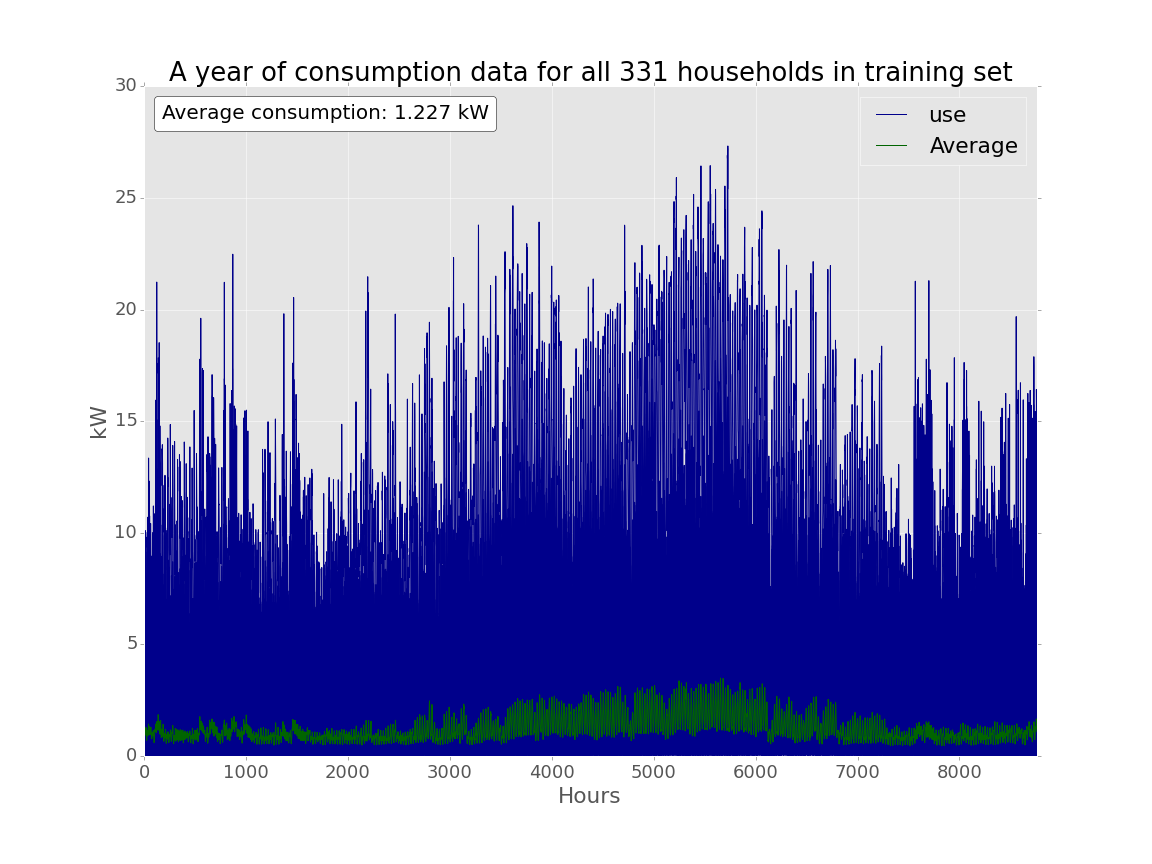
\includegraphics[scale=0.30]{./figures/houseuse}
	\caption{Training households, 2014}
	\label{fig:houseuse}
\end{figure}

As seen from the figure \ref{fig:houseuse}, some houses end up using almost 10 times more elecricity than the average household. These households have an impact to focus less on the more generalized households. Presumably these households are not of interest for Greenely or the generalized result in which we would want to classify. Here the assumption has been that these households are more of industrial size, although not nearly enough power consumption to be compared to, but acting more of a reference for which households have been investigated.

\begin{figure}[H]
	\centering
	\begin{minipage}{.5\textwidth}
		\centering
		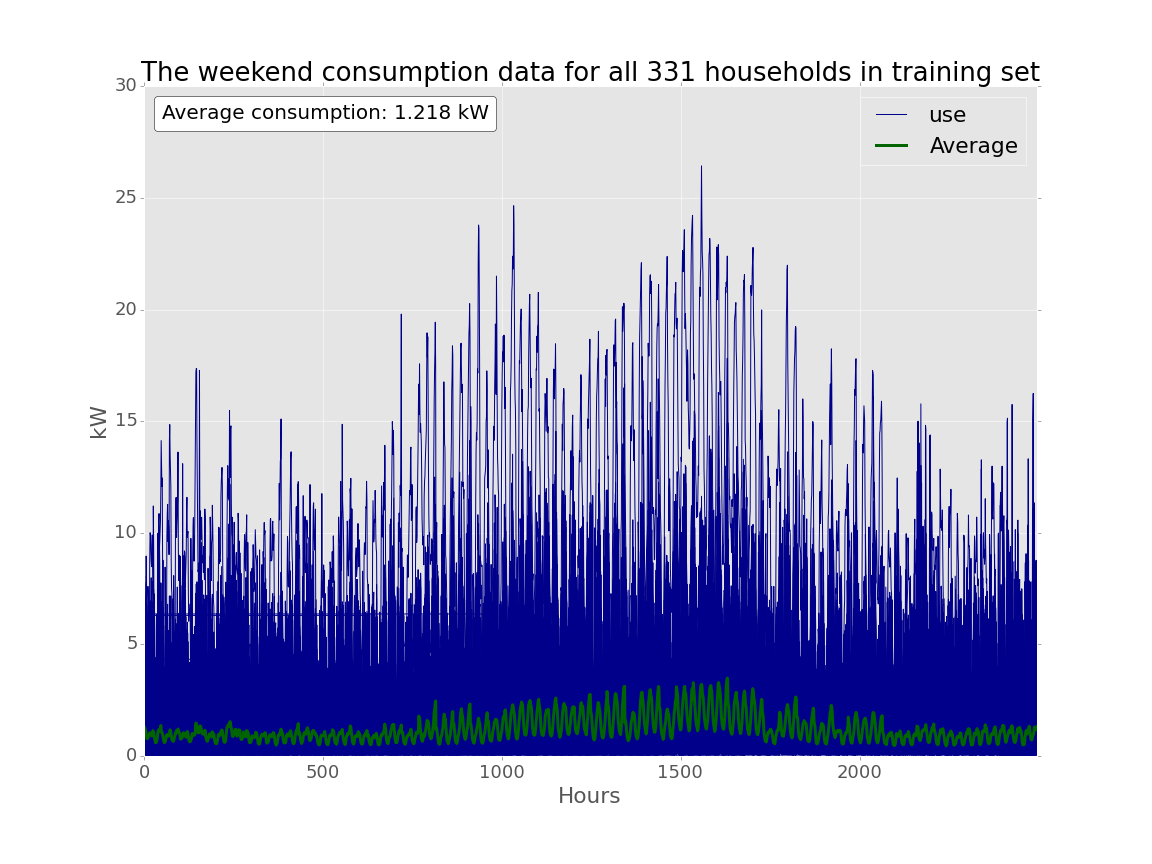
\includegraphics[scale=0.19]{./figures/weekendhouseuse}
		%\label{fig:test6}
	\end{minipage}%
	\begin{minipage}{.5\textwidth}
		\centering
		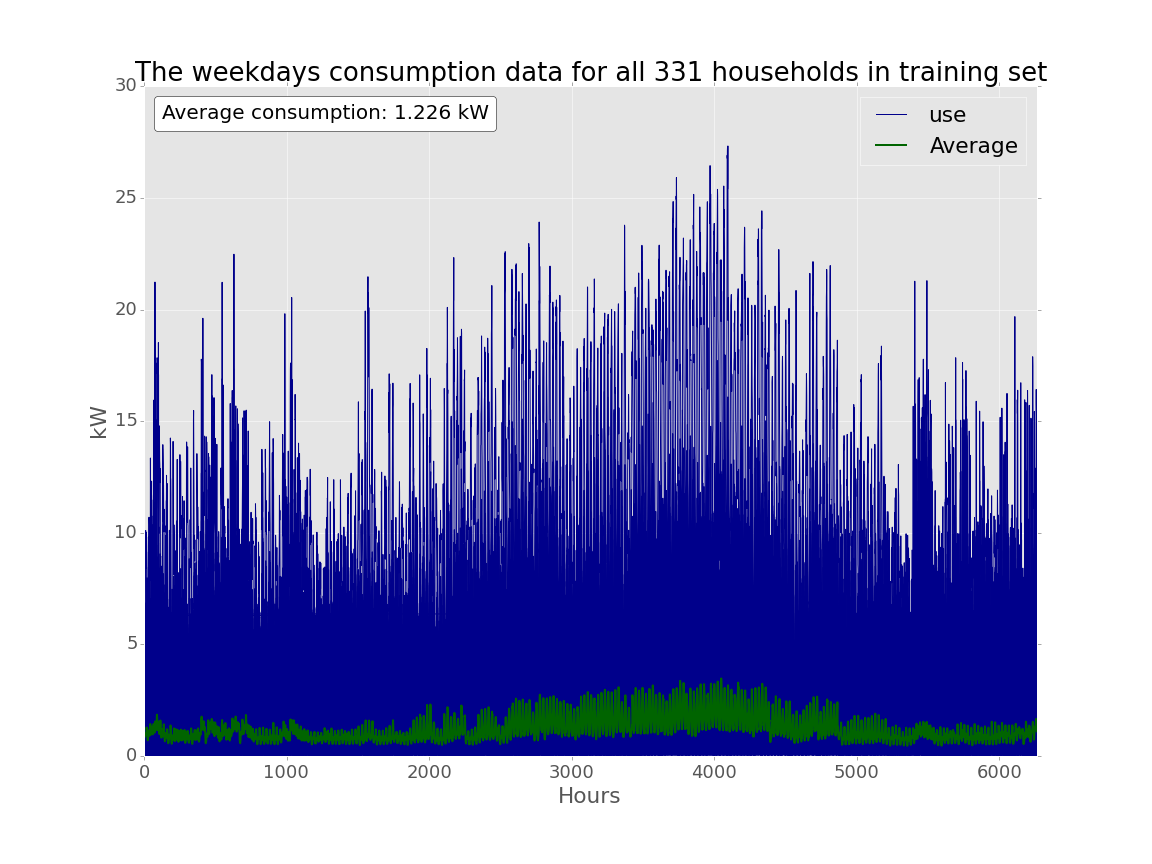
\includegraphics[scale=0.19]{./figures/weekdayshouseuse}
		%\label{fig:test5}
	\end{minipage}
	\caption{This figure shows two plots representing the weekday and weekend datasets. The datasets are compressed of a whole year of weekdays and weekends respectively. The left plot have values for all the hours of the weekends for a year 2496 hours. The right plot consists of hourly readings of 6240 hours.}
	\label{fig:weekend_day}
\end{figure}

From the figure above \ref{fig:weekend_day}, we can see that the left plot which has the weekends, consists of peaks of consumption. In comparison with the right plot, where we have a more consistent behaviour of the household consumption. However, we note that energy consumption show that it is not significant enough to take into consideration. We conclude that the algorithm could find better shapes within the data when the dataset has been split, however there will probably be no seen affect from the energy consumption.

\begin{figure}[H]
	\centering
	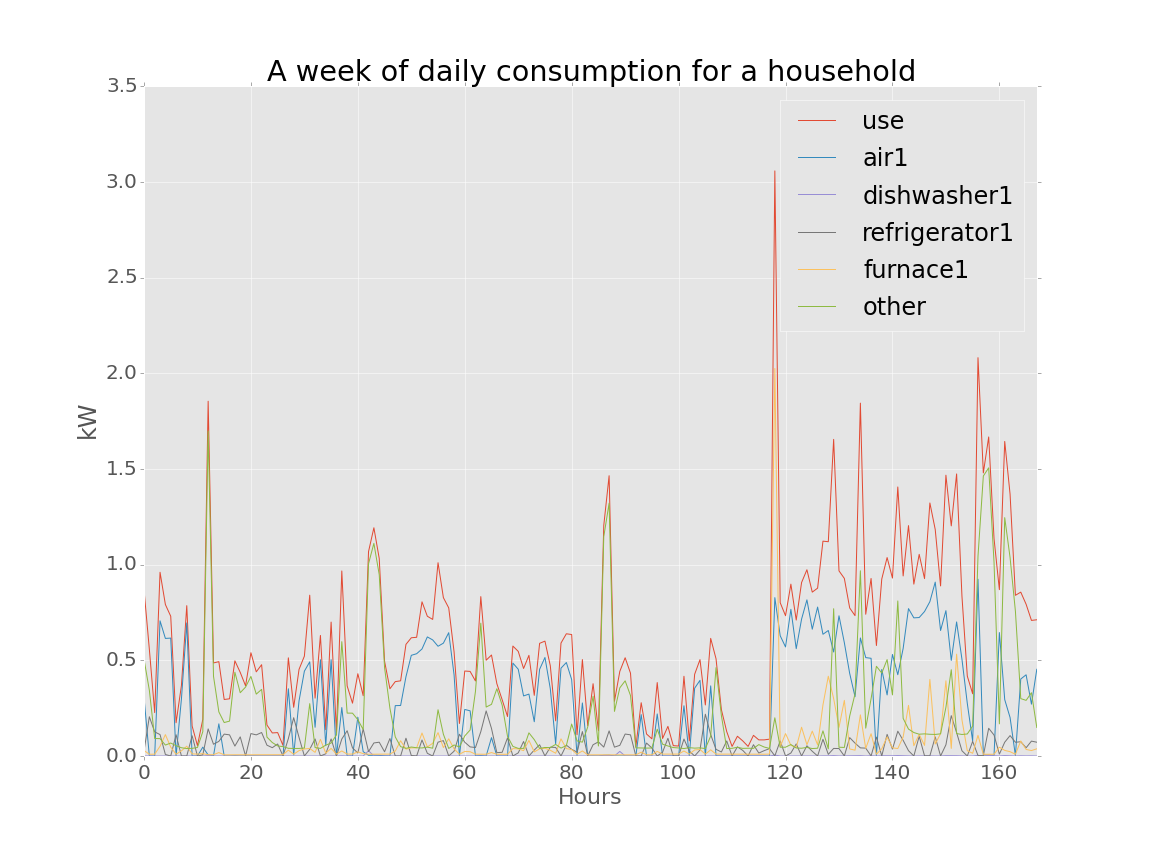
\includegraphics[scale=0.30]{./figures/weekconsump}
	\caption{A week of the consumption data for the appliances and whole-home usage}
	\label{fig:weekconsump}
\end{figure}

The figure shows consumption of the considered appliances. Pecan Street Inc's dataset is a great source of energy consumption data, however they have made a choice of registering average consumption of the particular appliance during that interval, with the aim that; if a refrigerator has been consuming one kilowatt per minute for 10 min and then gets turned off, it will be represented as $\frac{1}{10}$ instead of $\frac{1}{60}$, which could make the observation-based method flawed, as the assumption of precise measurements is the basis of the algorithm that Kotler et. al. presented \cite{DDSC}. 

\begin{figure}[H]
	\centering
		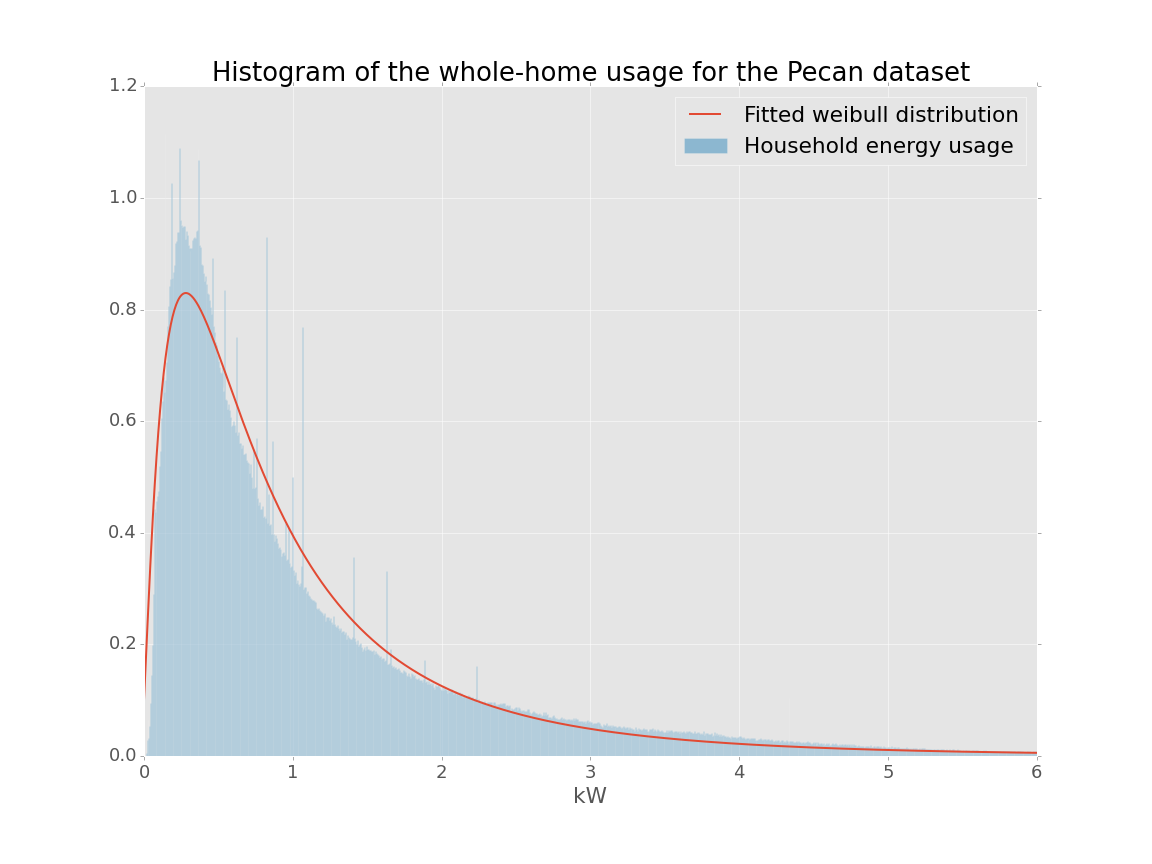
\includegraphics[scale=0.30]{./figures/new_histusage}
		\caption{Histogram of the household usage.}
		\label{fig:histuseage}
\end{figure}

The histogram in figure \ref{fig:histuseage} is presented to show that the usual consumption is substantially around the values 0.2 to 0.8 kW per hour. This is what Energy Information Administration \href{http://www.eia.gov/tools/faqs/faq.cfm?id=97&t=3}{EIA} presented in 2013 \cite{eia}, where they present the average consumption of an American household to 10,908 kilowatthours (kWh) which in turn corresponds to:

\begin{equation*}
	10.908 \textbf{kWh} / (24\times365) \textbf{h} = 1.245205479 \textbf{kW}
\end{equation*}

The average consumption for the Pecan Street households is 1.2244009446607182 \textbf{kW}, in the regard of average consumption the dataset can be seen as a good representation for a general household within the United States. Interesting to note is that the data can be fitted to a Weibull distribution, which has been used for providing dummy data.

\newpage
% --
\subsection{Discriminative Disaggregation via Sparse Coding}
\label{sec:ddsc}
This approach was presented in 2011 by J. Kolter MIT and Batr, Y.Nh from Stanford in \cite{DDSC}. It is based on improvements of single-channel source separation and enable a sparse coding algorithm to learn a model of each device's power consumption over a typical week. These learned models are then combined to predict the power consumption of different devices in previously unseen homes, using only their aggregate signal. Typically these algorithms have been used in audio signal separation, which usually has high temporal resolution (precision of measurement w.r.t. time) in contrast to low-resolution energy disaggregation; which impose new challenges within the field. Their algorithm shows an improvement of discriminatively training sparse coding dictionaries for disaggregation tasks. More specifically, they formulate the task of maximizing disaggregation as a structured prediction problem. 

The sparse coding approach to source separation, which forms for the basis for disaggregation, is to train separate models for each individual class $\mathbf{X}_i \in \mathbb{R}^{T\times m}$, where $T$ is the number of samples (hours in the given timeperiod) and $m$ is the number of features (households included) then use these models to separate an aggregate signal. Formally, sparse coding; models the $i$th data matrix using the approximation $\mathbf{X}_i \approx \mathbf{B}_i\mathbf{A}_i$ where the columns of $\mathbf{B}_i \in \mathbb{R}^{T \times n}$ contain a set of $n$ basis functions, also called the dictionary, and the columns of $\mathbf{A}_i \in \mathbb{R}^{n \times m}$ contain the activations of these basis functions, see section \ref{sec:scnn} for more detail. The data input is describe below:

\begin{itemize}
	\item{We define one class (e.g. heater) $\mathbf{X}_i \leftarrow 1,\dots,
		k$}
	\item{Where $\mathbf{X}_i \in \mathbb{R}^{T \times m}$, ex: week $T=24\times7=168$ of $m$ houses}
	\item{\textbf{One} aggregated household $\bar{\mathbf{X}} \leftarrow \sum_{i:k} \mathbf{X}_i$}
	\item{Assuming we have individual energy readings $\mathbf{X}_1,\dots,\mathbf{X}_k$}
	\item{Sparse encode $\mathbf{A},\mathbf{B}$ such that $(n \gg m,T)$}
	\item{Goal: test with new data $\bar{\mathbf{X}}'$ to components
		$\mathbf{X}_1',\dots,\mathbf{X}_k'$}
\end{itemize}

Sparse Coding additionally imposes the constraint that the activations $\mathbf{A}_i$ be sparse, i.e., that they contain mostly zero entries. This allows for learning \textit{overcomplete} sets of representations of the data (more basis functions than the dimensionality of the data, $n \gg m,T$). This makes sparse coding interesting for the field of energy disaggregation since the input data (energy consumption) is inherently positive. They also impose that the activations and dictionaries (bases) be non-negative, presented by \cite{hoyer} as non-negative sparse coding, see section \ref{sec:nnsc} for more detail. The non-negative sparse coding objective

\begin{equation}
\min_{\mathbf{A} \geq 0} \norm{\mathbf{X}_i - \mathbf{B}_i\mathbf{A}}_F^2 + \lambda \sum_{p,q} \mathbf{A}_{pq} \quad \text{subject to} \quad \norm{\mathbf{b}_i^{(j)}}_2 \leq 1, j=1,\dots,n
\end{equation}

where $\mathbf{X}_i,\mathbf{A}_i$ and $\mathbf{B}_i$ are defined as above, while $\lambda \in \mathbb{R}_+$ is a regularization parameter and norms defined as in beginning of section 2 \ref{sec:theoretical}. The sparse coding optimization problem is convex for each optimization-variable whilst holding the other variable fixed. The most common technique is to alternate between minimizing the objective over $\mathbf{A}_i$ and $\mathbf{B}_i$ \cite{DDSC}.

When the representations have been trained for each of the classes (appliances), we concatenated the bases to form a single joint set of basis functions and solve a disaggregation for a new aggregate signal $\bar{\mathbf{X}} \in \mathbb{R}^{T\times m'}$ using the procedure presented below. 

\begin{equation}
\label{eq:f}
\begin{aligned}
\hat{\mathbf{A}}_{1:k}  & = \arg \! \min_{\mathbf{A_{1:k}} \geq 0} \norm{\bar{\mathbf{X}}-\left[\mathbf{B}_1 \cdots \mathbf{B}_k\right]  
		\begin{bmatrix}
		\mathbf{A}_1 \\
		\vdots \\
		\mathbf{A}_k
		 \end{bmatrix}
	}_F^2 + \lambda \sum_{i,p,q}(\mathbf{A}_i)_{pq} \\
 & \vcentcolon= \arg \! \min_{\mathbf{A_{1:k}} \geq 0} F(\bar{\mathbf{X}},\mathbf{B}_{1:k},\mathbf{A}_{1:k})
\end{aligned}
\end{equation}

where $\mathbf{A}_{1:k}$ is denoted as $[\mathbf{A}_1,\dots,\mathbf{A}_k]$ and we abbreviate the optimization objective as $F(\bar{\mathbf{X}},\mathbf{B}_{1:k},\mathbf{A}_{1:k})$. We then predict the $i$th component of the signal to be 

\begin{equation}
\hat{\mathbf{X}}_i = \mathbf{B}_i \hat{\mathbf{A}_i}.
\end{equation}

The intuition is that if $\mathbf{B}_i$ is trained to reconstruct the $i$th class with small activation, then it should better represent the $i$th portion of the aggregate signal than all other bases $\mathbf{B}_j$ for $j\neq i$. Henceforth they construct a way of evaluating the quality of the resulting disaggregation (\textit{disaggregation error})

\begin{equation}
\label{eq:diserr}
E(\mathbf{X}_{1:k},\mathbf{B}_{1:k}) \vcentcolon= \sum_{i=1}^k \frac{1}{2} \norm{\mathbf{X}_i - \mathbf{B}_i \hat{\mathbf{A}}_i}_F^2 \ \text{s.t.} \ \hat{\mathbf{A}}_{1:k} = \arg \! \min_{\mathbf{A_{1:k}} \geq 0} F\left( \sum_{i=1}^k \mathbf{X}_i,\mathbf{B}_{1:k},\mathbf{A}_{1:k} \right),
\end{equation}

which quantifies the reconstruction process for each individual class when using the activations obtained only via the aggregated signal.

\subsubsection{Structured prediction for Discriminative Disaggregation Sparse Coding}

One of the issues that Andrew Ng and J.Zico Kotler point out, using Sparse Coding, the training is solely done for each appliance at hand when the whole-home consumption from consumers have a large variance, as can be seen in figure \ref{fig:houseuse}. The method revolves around training each individual class to produce a small disaggregation error. It is furthermore hard to optimize the disaggreagtion error direcly over the basis $\mathbf{B}_{1:k}$, ignoring the dependance of $\hat{\mathbf{A}}_{1:k}$ on $\mathbf{B}_{1:k}$, resolving for the activations  $\hat{\mathbf{A}}_{1:k}$ ; thus ignoring the dependance of $\hat{\mathbf{A}}_{1:k}$ on $\mathbf{B}_{1:k}$, which loses much of the problem's structure and this approach performs very poorly in practice.

In their paper they define an augmented regularized disaggregation error objective
\begin{equation}
\label{eq:regerror}
\begin{aligned}
\tilde{E}_{reg}(\mathbf{X}_{1:k},\mathbf{B}_{1:k},\tilde{\mathbf{B}}_{1:k})  & \vcentcolon=  \sum_{i=1}^k \left( \frac{1}{2} \norm{\bar{\mathbf{X}}-\mathbf{B}_i  \hat{\mathbf{A}}_i}_F^2 + \lambda \sum_{i,p,q}(\hat{\mathbf{A}}_i)_{pq} \right) \\
& \text{subject to } \hat{\mathbf{A}}_{1:k} = \arg \! \min_{\mathbf{A_{1:k}} \geq 0} F\left(\sum_{i=1}^k \mathbf{X}_i,\tilde{\mathbf{B}}_{1:k},\mathbf{A}_{1:k}\right),
\end{aligned}
\end{equation}

where the $\mathbb{B}_{1:k}$ bases (referred to as the reconstruction basis) are the same sas those learned from sparse coding while the $\tilde{\mathbf{B}}_{1:k}$ bases (disaggreagtion bases) are discrimintively optimized in order to move $\hat{\mathbf{A}}_{1:k}$ close to $\mathbf{A}_{1:k}^{\bigstar}$, without changing these targets. For more detail regarding this section, see Kotler et.al. page four \cite{DDSC}. Here they describe that we seek bases $\tilde{\mathbf{B}}_{1:k}$ such that (ideally)

\begin{equation}
\mathbf{A}_{1:k}^\bigstar = \arg \! \min_{\mathbf{A_{1:k}} \geq 0} F ( \bar{\mathbf{X}}, \tilde{\mathbf{B}}_{1:k},\mathbf{A}_{1:k}).
\end{equation}

In paper \cite{DDSC} it is noted that many methods can be applied to the prediction problems. They chose a structured prediction algorithm presented in Collins 2005 \cite{collins}. Given some value of the parameters $\tilde{\mathbf{B}}_{1:k}$, we first compute $\hat{\mathbf{A}}$ using equation \ref{eq:f}. The perceptron update with a step size $\alpha$ is now

\begin{equation}
\tilde{\mathbf{B}}_{1:k} \leftarrow \tilde{\mathbf{B}}_{1:k} - \alpha \left( \Delta_{\tilde{\mathbf{B}}_{1:k}} F(\bar{\mathbf{X}},\tilde{\mathbf{B}}_{1:k},\mathbf{A}_{1:k}^\bigstar) - \Delta_{\tilde{\mathbf{B}}_{1:k}} F(\bar{\mathbf{X}},\tilde{\mathbf{B}}_{1:k},\hat{\mathbf{A}}_{1:k} \right)
\end{equation}

or to be more explicit by defining the concatenated matrices $\tilde{\mathbf{B}} = [ \tilde{\mathbf{B}}_1 \cdots \tilde{\mathbf{B}}_k ], \mathbf{A}^\bigstar = [{\mathbf{A}_1^\bigstar}^T \cdots{\mathbf{A}_k^\bigstar}^T ]$ (similar for $\hat{\mathbf{A}}$),

\begin{equation}
\label{eq:4b}
\tilde{\mathbf{B}} \leftarrow \left[ \tilde{\mathbf{B}} - \alpha \left( (\bar{\mathbf{X}} - \tilde{\mathbf{B}}\hat{\mathbf{A}})\hat{\mathbf{A}}^T - (\bar{\mathbf{X}}-\tilde{\mathbf{B}}\mathbf{A}^\bigstar)(\mathbf{A}^\bigstar)^T \right) \right]_+
\end{equation}

In conjuncting with the equation above, we keep the postive values of $\tilde{\mathbf{B}}_{1:k}$ and re-normalize each column to have unit norm (step 4c in DDSC algorithm \ref{alg:ddsc}). 

\subsection{Implementation}
\label{sec:implementation}
The vast increase of interest within Machine Learning and the applications that it can bring in the digitized aged have made it possible for many Open Source libraries used for Sparse Coding. In this thesis \textsc{Python} has been used as a means of implementation. The source code for the implemented algorithms can be found in section \ref{sec:appendix} and the mathematical notation is found below in section \ref{sec:implemented}. Below is a list of libraries connected to Machine Learning using \textsc{Python} and the argumentation behind the libraries chosen.

\begin{itemize}
	\item{NeuroLab, Deep Learning}
	\item{Theano, Deep Learning}
	\item{Statsmodels, Statistical library}
	\item{Scikit-Learn, General Machine Learning \cite{scikit}}
	\item{Librosa, Signal processing library}
\end{itemize} 

Neurolab and Theano are the more low-level deep learning libraries, that provide the users with lots of options, but however needs a great deal of knowledge in both python and deep learning. Statsmodels is a \textsc{Python} module that allows users to explore data, estimate statistical models, and perform statistical tests. We chose to use the standard Machine Learning library \href{www.scikit-learn.org}{Scikit-Learn}  and \href{http://theremin.ucsd.edu/~bmcfee/librosadoc/index.html}{Librosa}. Scikit-Learn is the go to library when it comes to Machine Learning with \textsc{Python} as it provides a whole set of constructs to build from and to test the algorithms, as well as a vast community. The Librosa library was chosen as it exclusively provides a set for signal processing methods. Although the DDSC algorithm relies on standard methods, the libraries provide a means to proven and tested algorithms. J.Zico Kotler et. al. explain that they had space constraints to preclude a full discussion about the implementation details. They however present the algorithms used, as specified from Kotler et. al. \cite{DDSC} the procedure of DDSC we have implemented a coordinate descent for the steps 2a and 4a in algorithm \ref{alg:ddsc} using Scikits module \href{http://scikit-learn.org/stable/modules/generated/sklearn.decomposition.SparseCoder.html#sklearn.decomposition.SparseCoder}{SparseCoder} and using Librosa to decompose for retreiving the activation matrix. They also refer to Hoyer's paper \cite{hoyer} on multiplicative non-negative matrix factorization update to solve step 2b. The algorithm is presented in \ref{alg:nnsc} as non-negative matrix factorization. The step 4b in the algorithm is explained in equation \ref{eq:4b} as a means to update the basis, and is a straight forward implementation.


\subsection{Implemented Algorithms}
\label{sec:implemented}
The source code for the Non-Negative Sparse-Coding algorithm can be found in Appendix \ref{sec:sc_nnsc} and the source code for the Discriminative Disaggregation algorithm can be found in Appendix \ref{sec:sc_dd}.

\subsubsection{Non-Negative Sparse-Coding}
\label{alg:nnsc}
\begin{algorithm}[H]
	\caption{Non-Negative Sparse Coding}

	\SetKwInOut{Input}{input}
	\Input{Solving the problem of equation \ref{eq:nnsc} in the section for Non-Negative Sparse Coding, \ref{sec:nnsc}}
	\begin{algorithmic}[1]
		\Statex{Interate until convergence:}
		\State{Set positive values for $\mathbf{B}^0$ and $\mathbf{A}^0$, and also set $t=0$.}
		\State{a) $\mathbf{B}' = \mathbf{B}^t - \mu(\mathbf{B}^t \mathbf{A}^t-\mathbf{X})(\mathbf{A}^t)^T$.}
		\Statex{b) Set negative values of $\mathbf{A}'$ to zero.}
		\Statex{c) Rescale $\mathbf{B}'$ to unit norm, and then set $\mathbf{B}^{t+1}=\mathbf{B}'$.}
		\Statex{d) $\mathbf{A}^{t+1}=\mathbf{A}^t.*((\mathbf{B}^{t+1})^T\mathbf{A})./((\mathbf{B}^{t+1})^T(\mathbf{B}^{t+1}\mathbf{A}^t+\lambda))$.}
		\Statex{e) Convergence if $\norm{ \mathbf{A}^{t+1} - \mathbf{A}^{t} } < \epsilon$}
		\Statex{f) Increment t.}
		
	\end{algorithmic}
\end{algorithm}

\subsubsection{Discriminative Disaggregation via Sparse Coding}
\label{alg:ddsc}
%
\begin{algorithm}[H]
\caption{Discriminative Disaggregation via Sparse Coding}
\SetKwInOut{Input}{input}
\Input{data points for each individual source $\mathbf{X}_i \in
\mathbb{R}^{T \times m}, i = 1:k,$ regularization $\lambda
\in \mathbb{R}_+$, with gradient step size $\alpha \in \mathbb{R}_+$.}
\begin{algorithmic}[1]
\Statex{  \textbf{Sparse coding pre-training:}}
\Statex{  \hspace{0.2in} 1. Initalize \textbf{B}$_i$, $\mathbf{A}_i \ \geq 0$, scale columns $\mathbf{B}_i$ s.t. $\norm{ \mathbf{b}_i^{(j)}}_2 =1$}
\Statex{ \hspace{0.2in} 2. For each $i=1,\dots,k,$ iterate until convergence: }
\Statex \hspace{0.4in} $\mathbf{A_i} \leftarrow \arg \! \min_{\mathbf{A} \geq 0} \norm{\mathbf{X}_i - \mathbf{B}_i\mathbf{A}}_F^2 + \lambda \sum_{p,q} \mathbf{A}_{pq}$
\Statex \hspace{0.4in} $\mathbf{B}_i \leftarrow  \arg \! \min_{\mathbf{B} \geq 0,\norm{\mathbf{b}^{(j)}}_2 \leq 1} \norm{\mathbf{X}_i - \mathbf{B} \mathbf{A}_i }_F^2$
\Statex \textbf{Discriminative disaggregation training:}
\Statex  \hspace{0.2in} 3. Set $\mathbf{A}_{1:k}^* \leftarrow \mathbf{A}_{1:k},\hat{\mathbf{B}}_{1:k} \leftarrow \mathbf{B}_{1:k}.$
\Statex  \hspace{0.2in} 4. Iterate until convergence:
\Statex \hspace{0.4in} $\hat{\mathbf{A}}_{1:k} \leftarrow \arg \! \min_{\mathbf{A}_{1:k} \geq 0} F\left( \bar{\mathbf{X}},\tilde{\mathbf{B}}_{1:k},\mathbf{A}_{1:k} \right)$
\Statex \hspace{0.4in} $\tilde{\mathbf{B}} \leftarrow \left[ \tilde{\mathbf{B}} - \alpha \left( (\bar{\mathbf{X}} - \tilde{\mathbf{B}}\hat{\mathbf{A}})\hat{\mathbf{A}}^T - (\bar{\mathbf{X}}-\tilde{\mathbf{B}}\mathbf{A}^\bigstar)(\mathbf{A}^\bigstar)^T \right) \right]_+$
\Statex \hspace{0.4in} $\forall \  i,j, \quad \mathbf{b}_i^{(j)} \leftarrow \mathbf{b}_i^{(j)} / \norm{\mathbf{b}_i^{(j)}}_2$
\Statex \textbf{Given aggregated test examples $\bar{\mathbf{X}}'$}
\Statex \hspace{0.2in} 5. $\hat{\mathbf{A}}'_{1:k} \leftarrow \arg \! \min_{\mathbf{A}_{1:k} \geq 0} F(\bar{\mathbf{X}}',\tilde{\mathbf{B}}_{1:k},\mathbf{A}_{1:k})$
\Statex \hspace{0.2in} 6. Predict $\hat{\mathbf{X}}_i' = \mathbf{B}_i\hat{\mathbf{A}}_i'$
\end{algorithmic}
\end{algorithm}

\newpage
\section{Results}
%• Results: What were the results? What could be deduced from the results? Uncertainty in
%the results? Do we now know everything?
%• Results: What were the results? What could be deduced from the results? Uncertainty in
%the results? Do we now know everything?
This section presents the performed experiments, along with their respective results and evaluations. We first present results based on a subset of the datasets in section \ref{sec:evaluation}. We then present predicted energy profiles and total energy profiles for the complete dataset in section \ref{sec:complete},  we then present the same experiments done on the different datasets in section \ref{sec:days_end}. Later, in section \ref{sec:a_b} the learned basis functions are presented and discussed. Lastly, in section \ref{sec:quant} we present a quantitative evaluation by looking at the error and accuracy results.

\subsection{Experimental setup}

The conducted work used the data set provided by Pecan Street, and pre-processed as described in \ref{sec:prep}. We look at time periods in blocks of one week and two weeks while trying to predict the individual device consumption over the time period; given only the whole-home signal. Imperatively, we focus on disaggregating data from homes that are absent from the training set, where 70\% were assigned as the training set and 30\% as the test set; thus, attempting to generalize over the basic category of devices, not just over different uses of the same device in a single house. We fit the parameters $\lambda,\alpha$ for regularization and stepsize  respectively using grid search, namely by chosing the best parameters from the search of a discrete set of empirical values.

Due to insufficient computational power, most of the tests have not been run using enough basis functions. We have chosen to go through with the setup, as we wanted to see temporal difference using this algorithm and not particularly wanted to perfect the setup. We chose to select only 67 houses out of the 331 houses that could have been used for the experiment from the set of 689 houses within the dataset. As we need to have more basis functions than the dimensionality of the data, we have chosen to use more basis functions than houses ($n > m$). We have also excluded a monthly prediction, as it would again cause computational issues. We have however provided one 24-hour prediction with a small subset of all of the datasets using enough basis functions to see that the algorithm can discriminate on all the datasets.

\subsection{Evaluation of algorithm}

\label{sec:evaluation}
Here we will present the results qualitively obtained by the method. First we begin by showing the predictions on a small subset of the data (30 houses), to see that the algorithm can actually discriminate the appliances at hand for all of the datasets that will be investigated. Then we proceed with the weekly prediction shown in figure \ref{fig:normal_168}, which shows the true energy consumed for a week, along with the energy consumption predicted by the algorithms. Next we present the results for a two week prediction, shown in figure \ref{fig:normal_360}. The figures also show two pie charts presenting the percentage use of each appliance, one of which is the true usage and the other shows the predicted usage. Furthermore we show the results obtained when splitting the dataset into two components, one containing the data from weekdays and one consisting out of only hourly readings from weekends.

\pagebreak[4]
\centerline{\textbf{$T=$24 hours and $m=$30 houses and $n=$250 basis functions}}
\begin{figure}[H]
		\centering
		\textbf{Week}\vspace{0.00001in}
		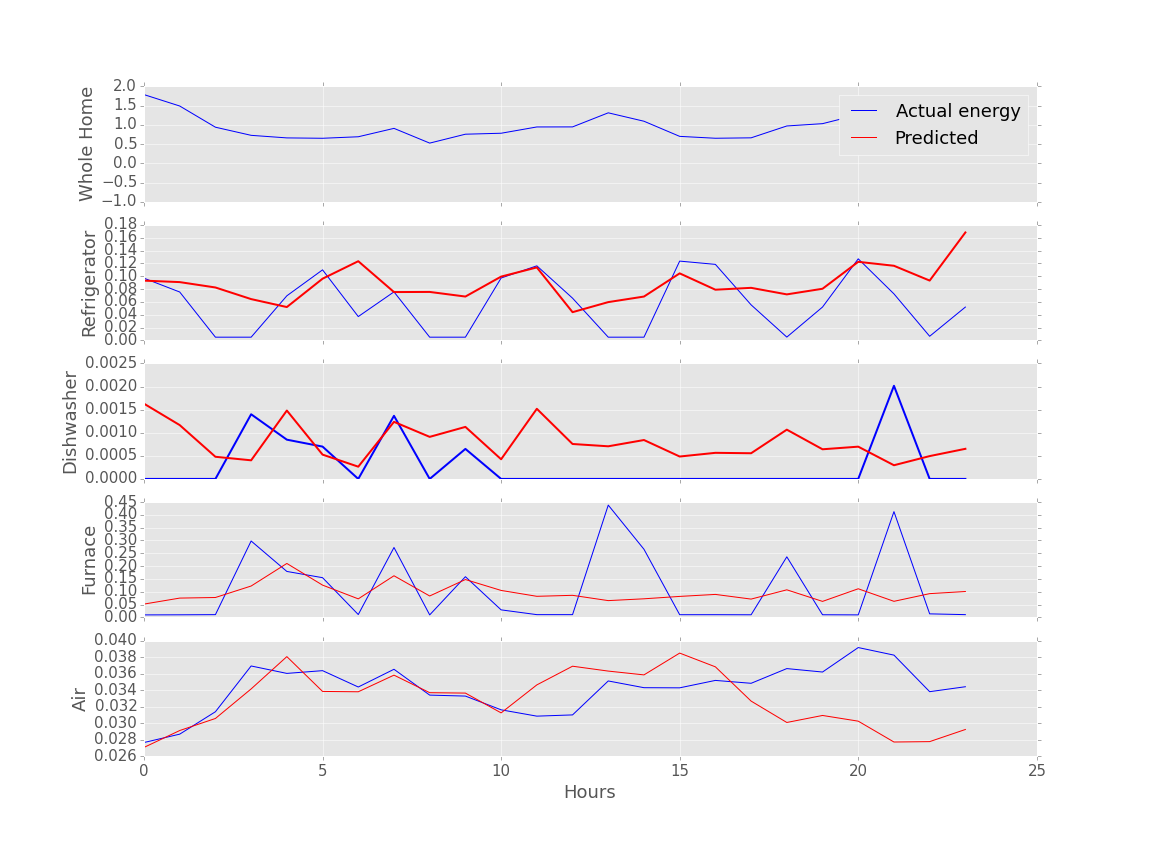
\includegraphics[width=\textwidth,height=8cm]{./figures/normal_250_24}
		%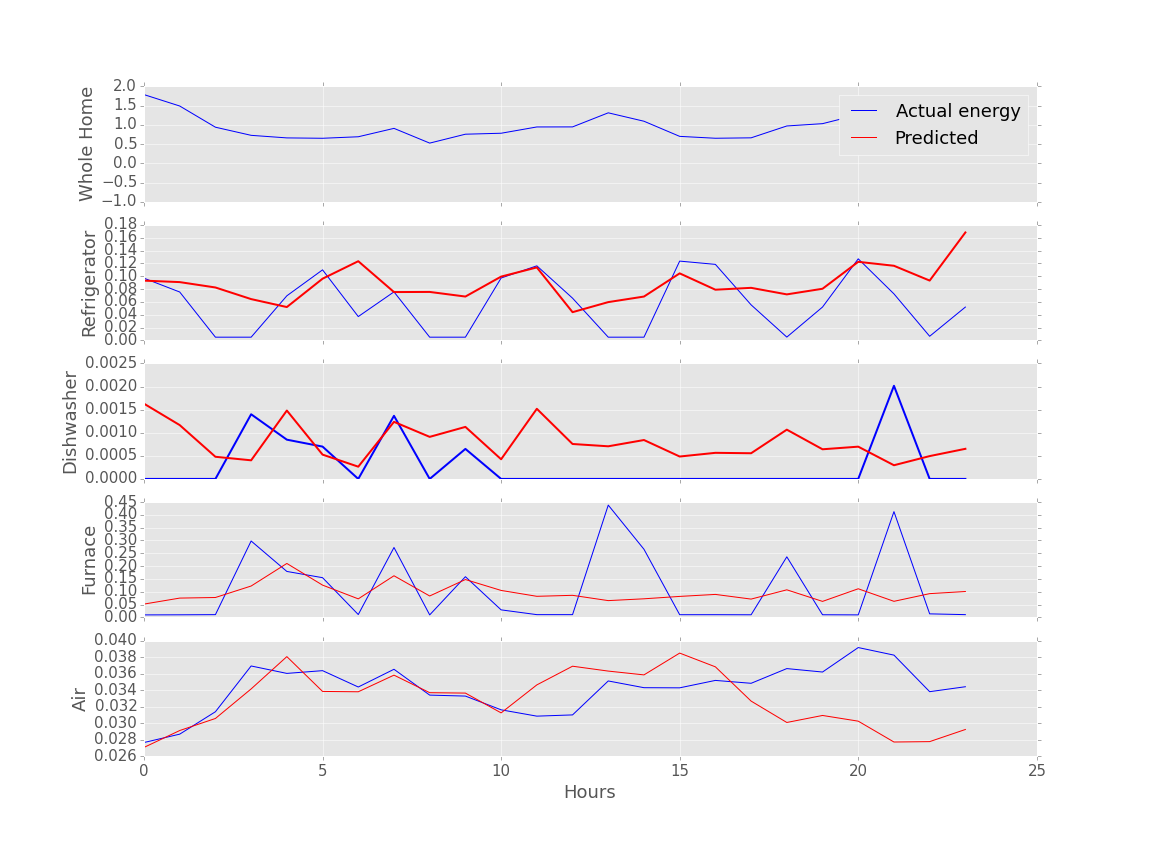
\includegraphics[scale=0.20]{./figures/normal_250_24}
\end{figure}
\begin{figure}[H]
		\centering
		\textbf{Weekdays}\vspace{0.00001in}
		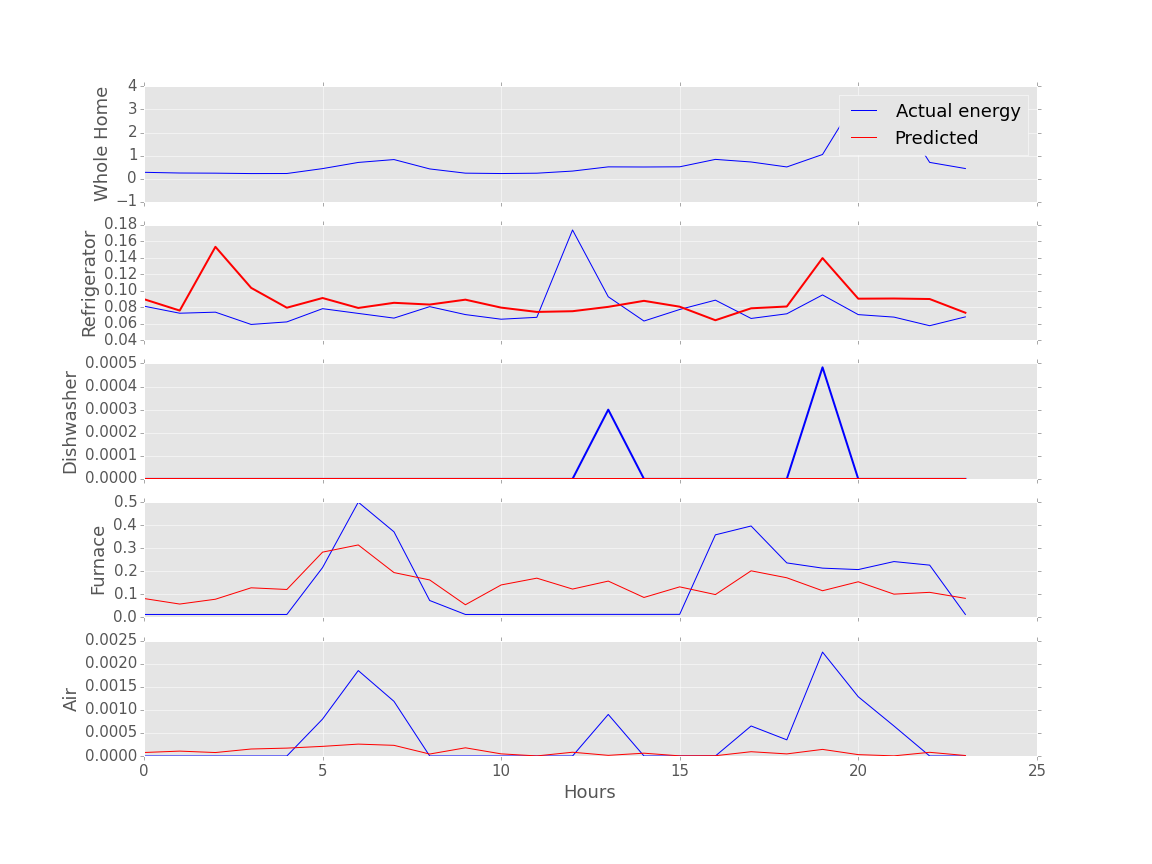
\includegraphics[width=\textwidth,height=8cm]{./figures/days_250_24}
	\end{figure}
\begin{figure}[H]
		\centering
		\textbf{Weekends}\vspace{0.00001in}
		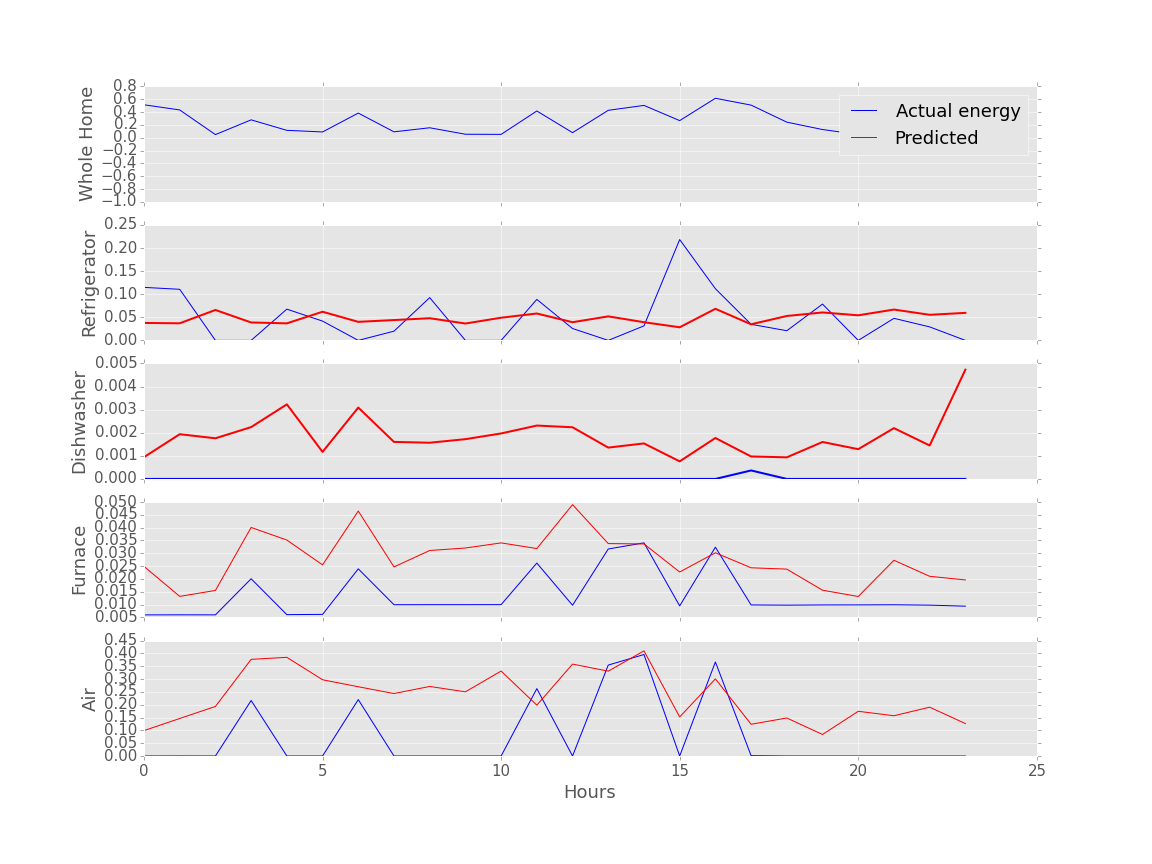
\includegraphics[width=\textwidth,height=8cm]{./figures/end_250_24}
\end{figure}
	
\begin{figure}[H]
	\caption{The figure shows the true usage (blue) and predicted energy consumption (red) of all of the appliances for all datasets. The left hand plot shows the whole dataset used in predicting the 24 hours. The middle plot shows the weekdays dataset being predicted for 24 hours and the right hand plot shows the prediction for the weekend dataset.}
	\label{fig:subset}
\end{figure}


In all the cases the algorithm has found basis functions and activations to represent an energy consumption profile of all of the appliances. This goes to show that the implementation of the algorithm has been successful and that the algorithms do serve their purpose, more on the evaluation on the different algorithms is done further down in section \ref{sec:quant}. Interesting to note is that the algorithm has found some of the energy profiles of some appliances. Looking at the plot to the bottom left we see that the prediction has actually been proved to be almost in line with the true profile for 10 of the data points (10 hours). We can also see that the algorithm can output completely different profiles by looking at the refrigerator for the weekdays dataset compared to that of the air-condition profile for the week dataset. 

\subsubsection{Results from the complete dataset}
\label{sec:complete}
\begin{figure}[H]
	\centering
	\textbf{$T=$168 hours and $m=$67 houses and $n=$80 basis functions}\par\medskip
	\begin{minipage}{.65\textwidth}
		\centering
		%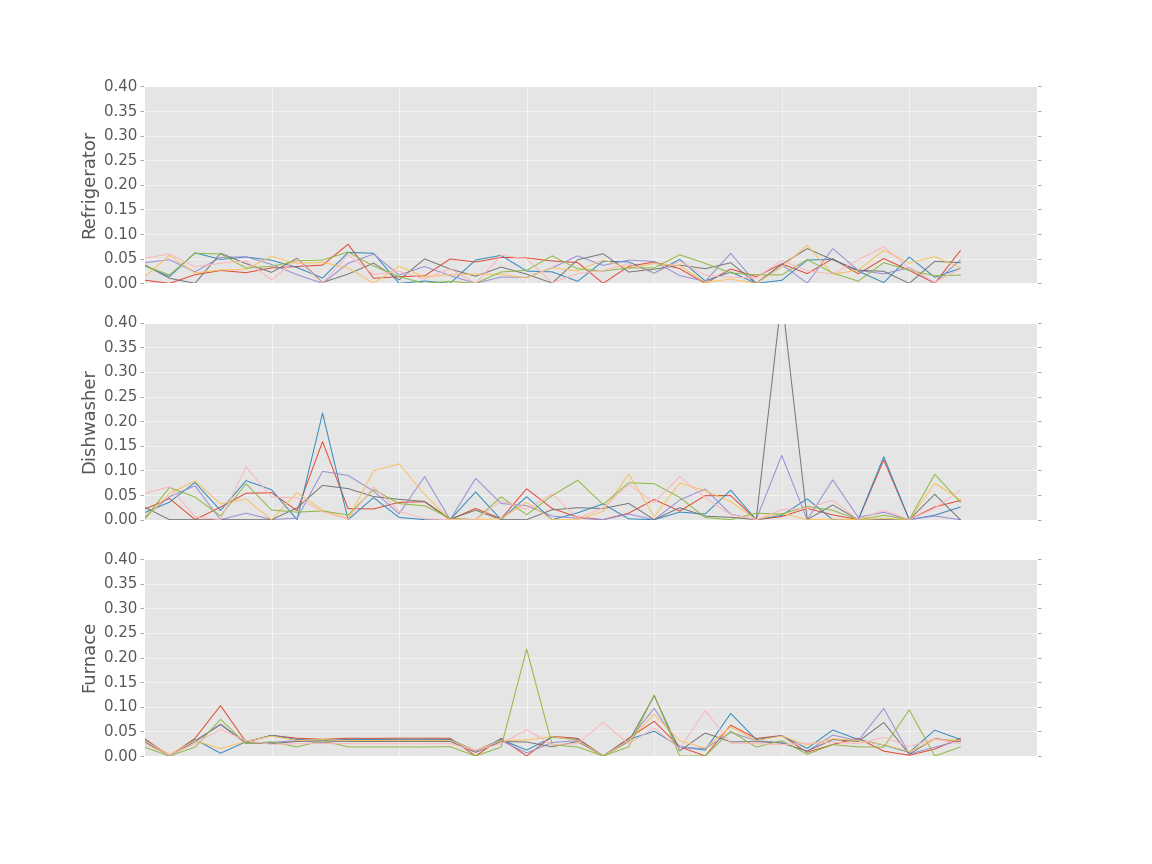
\includegraphics[scale=0.18]{./figures/app_basis}
		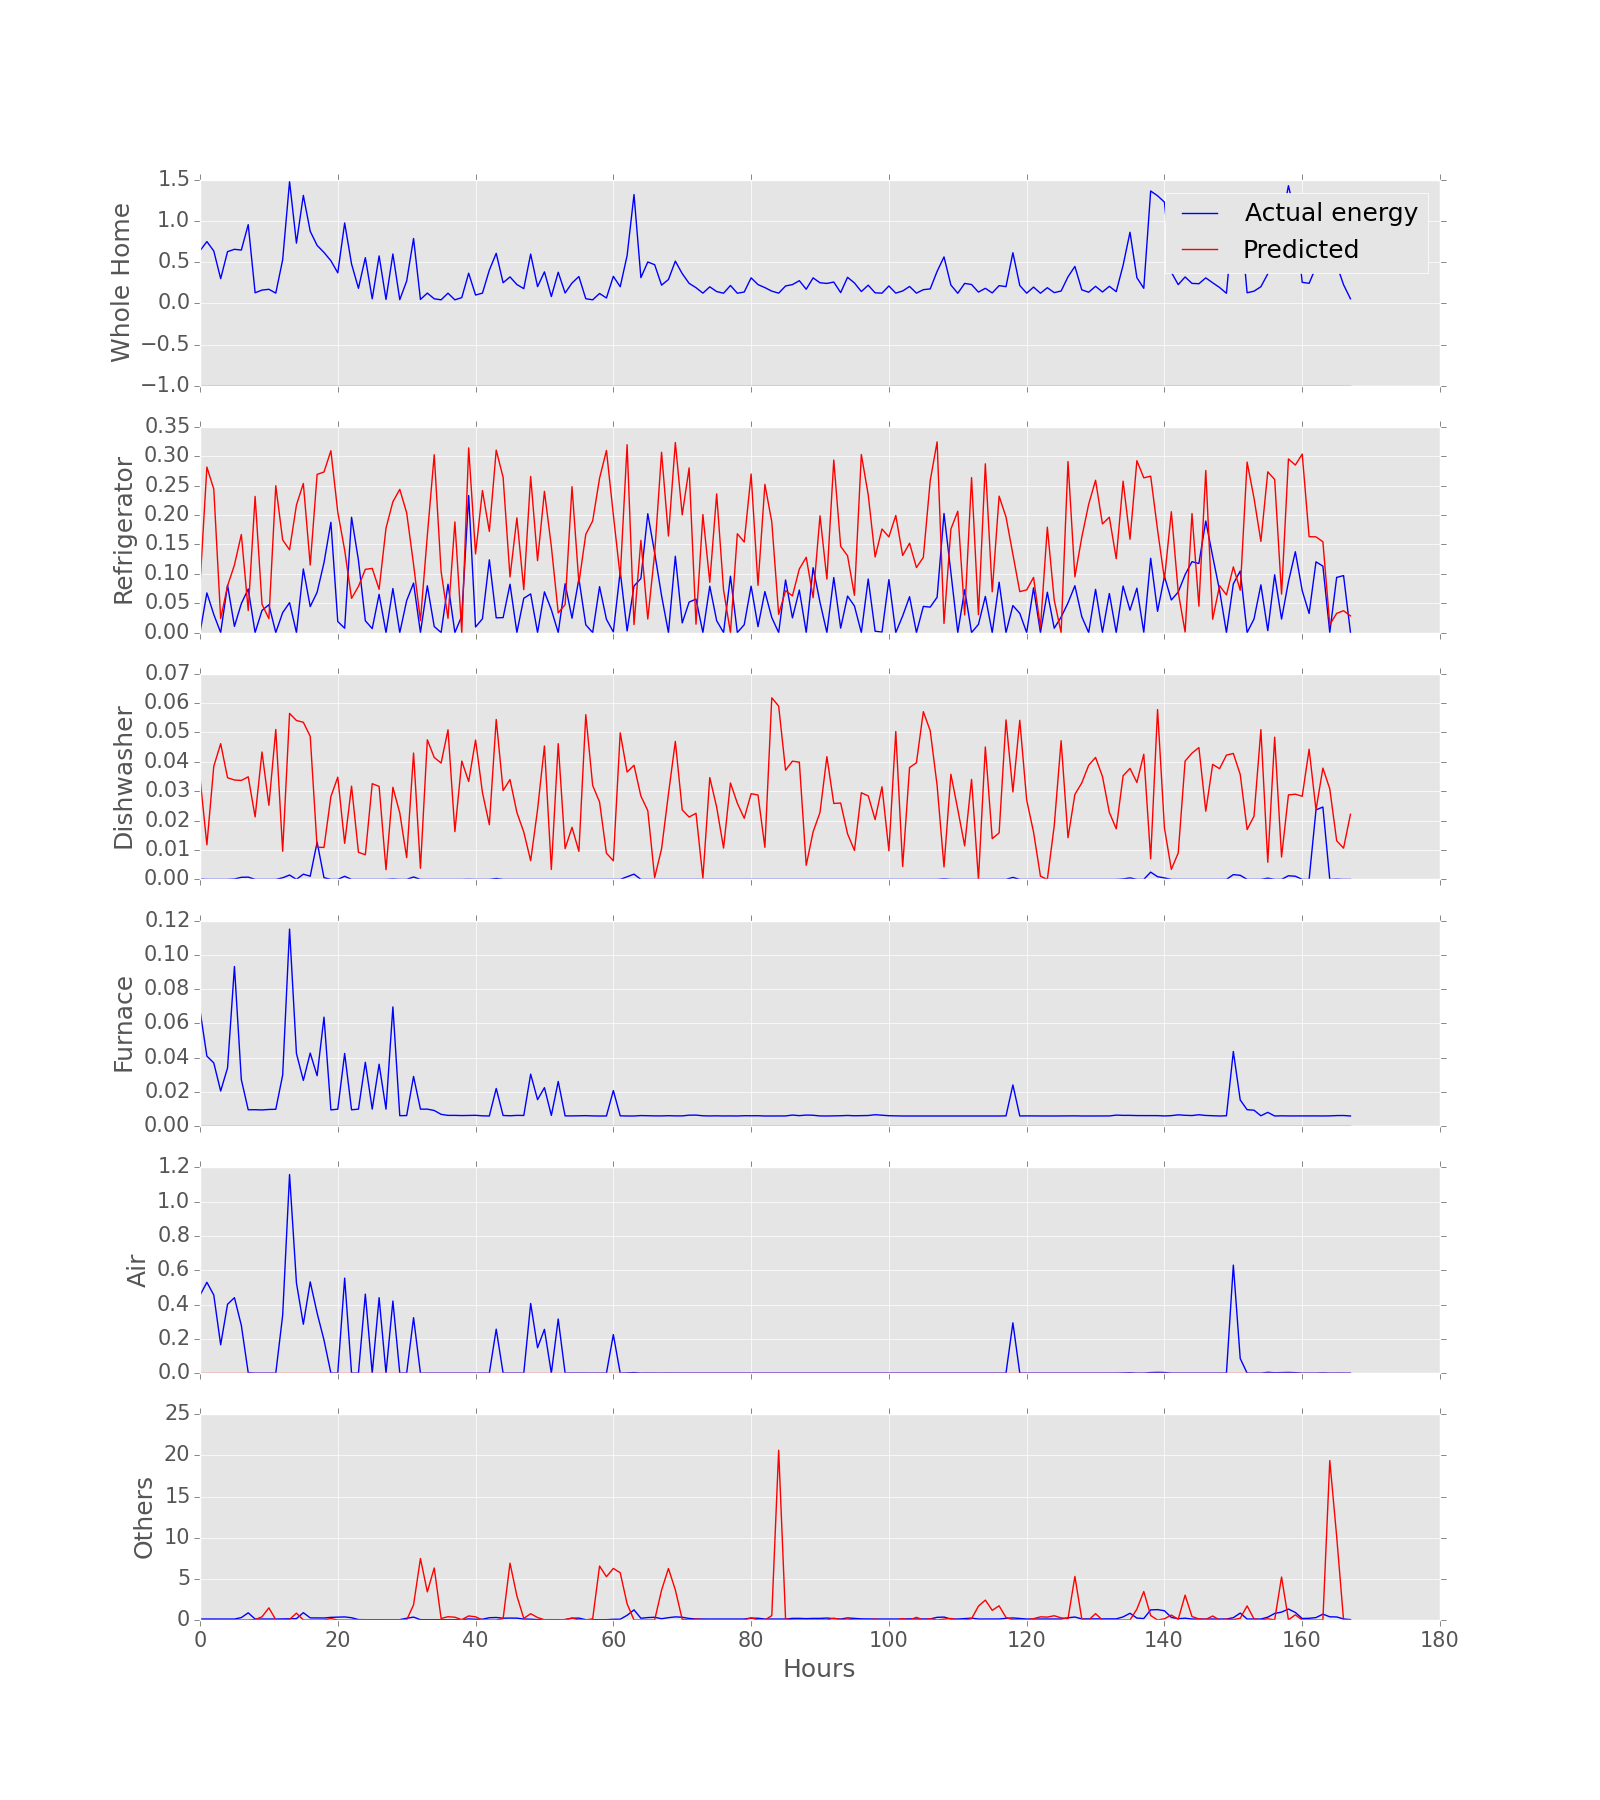
\includegraphics[width=\textwidth,height=10cm]{./figures/results/normal_appliances_67_168}
	%	\label{fig:test8}
	\end{minipage}%
	\begin{minipage}{.4 \textwidth}
		\centering
		%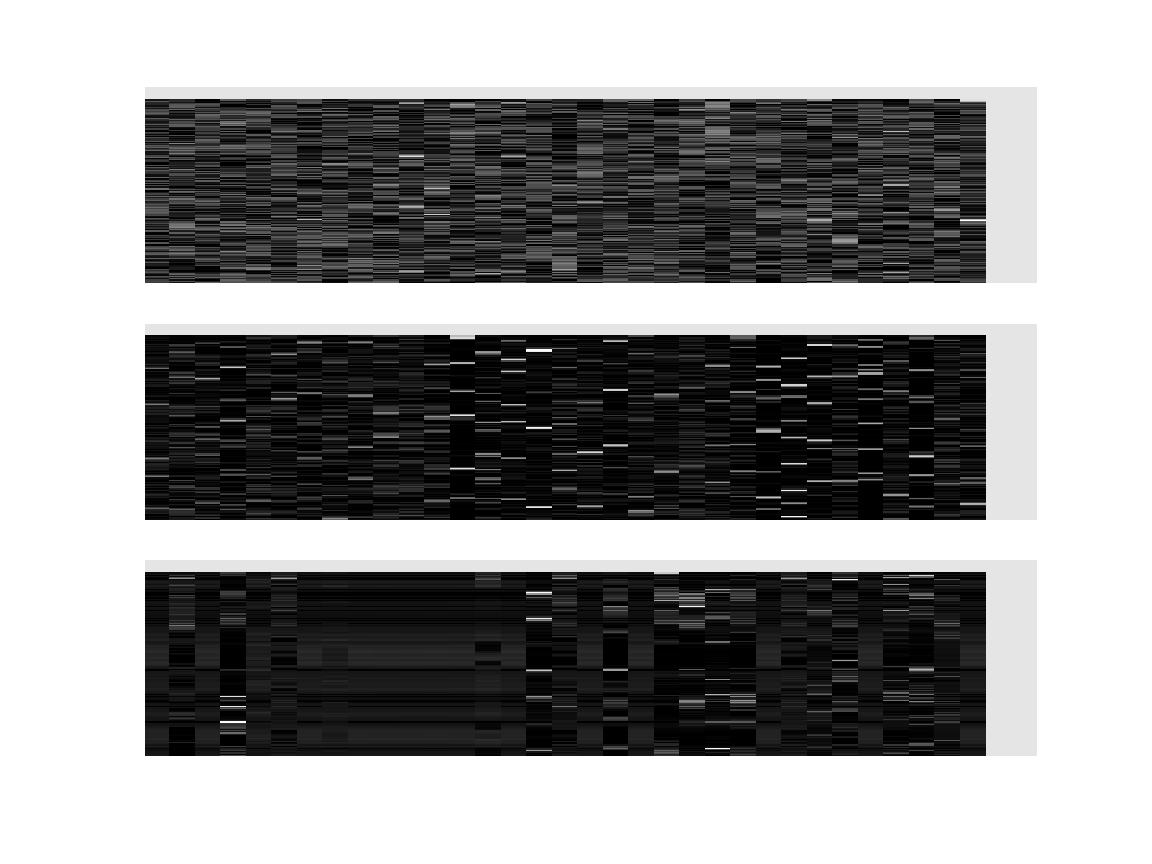
\includegraphics[scale=0.18]{./figures/basis}
		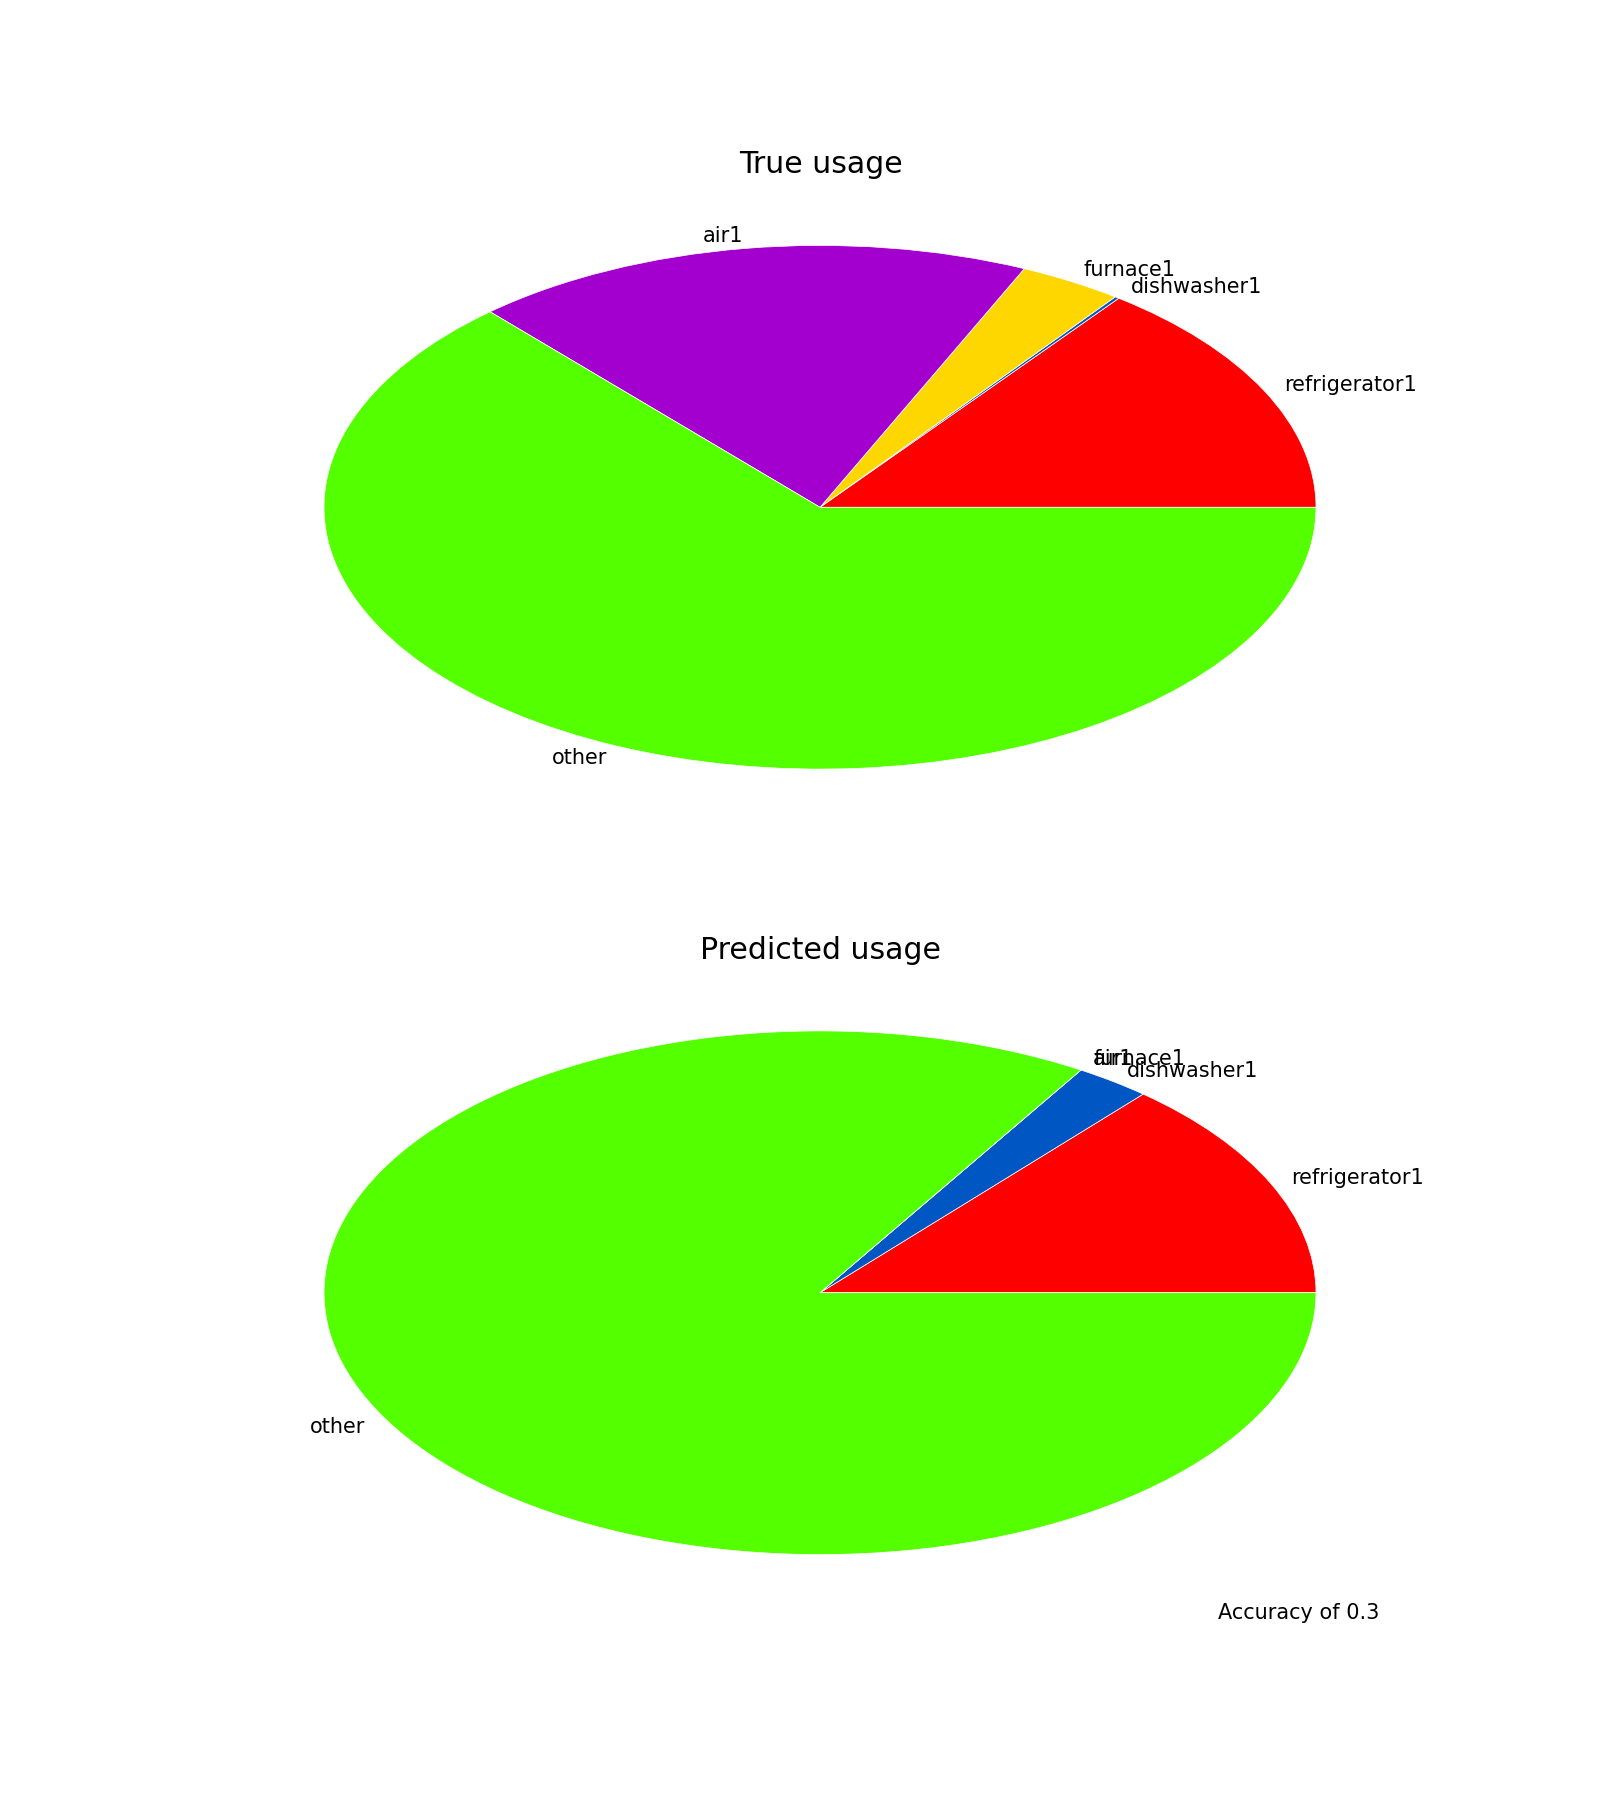
\includegraphics[width=\textwidth,height=10cm]{./figures/results/normal_pie_chart_67_168}
	%	\label{fig:test9}
	\end{minipage}
	\caption{Example of one house true energy profile and the predicted energy profile over a one week time period. The plot to the left shows true and predicted energy profiles. The plot to the right shows a pie chart of the total percentage that each appliance true usage and predicted usage.}
	\label{fig:normal_168}
\end{figure}

In most cases, the predicted values are quite poor, and the overall accuracy was 0.29, by the definition in equation \ref{eq:acc}. It seems as though the algorithm has not gotten any type of pattern but rather unique constant energy consumption for each appliance. Both the dishwasher and the refrigerator have a consistent shape of being volatile and almost like noise. One thing to note is the shape of the predicted usage of other appliances, this shape is highly complex due to its peak like behavior and is one shape that is hard to try to learn without using methods such as sparse coding which says that the algorithm can be used for predicting the shapes. Although it has overestimated the usage of other appliances as we can see in the pie charts. However it has completely not learnt that air or furnace has not been used at all, which is a failure in the results, and only the refrigerator has roughly the same amount of percentage usage as the true usage. The "other" appliances can be seen as a good result when representing a complex structure such as a dishwasher usage we have captured the structure of a "on" and "off" behavior, even though we did not use enough basis functions, we can still represent a structure like it. It is however not a good result when predicting each appliance as well as the overall energy usage. It heavily overestimates the usage of "other" appliances as well as assumes a significant higher consumption on both the "other" appliances and the dishwasher. 

\begin{figure}[H]
	\centering
	\textbf{$T=$360 hours and $m=$67 houses and $n=$144 basis functions}\par\medskip
	\begin{minipage}{.65\textwidth}
		\centering
		%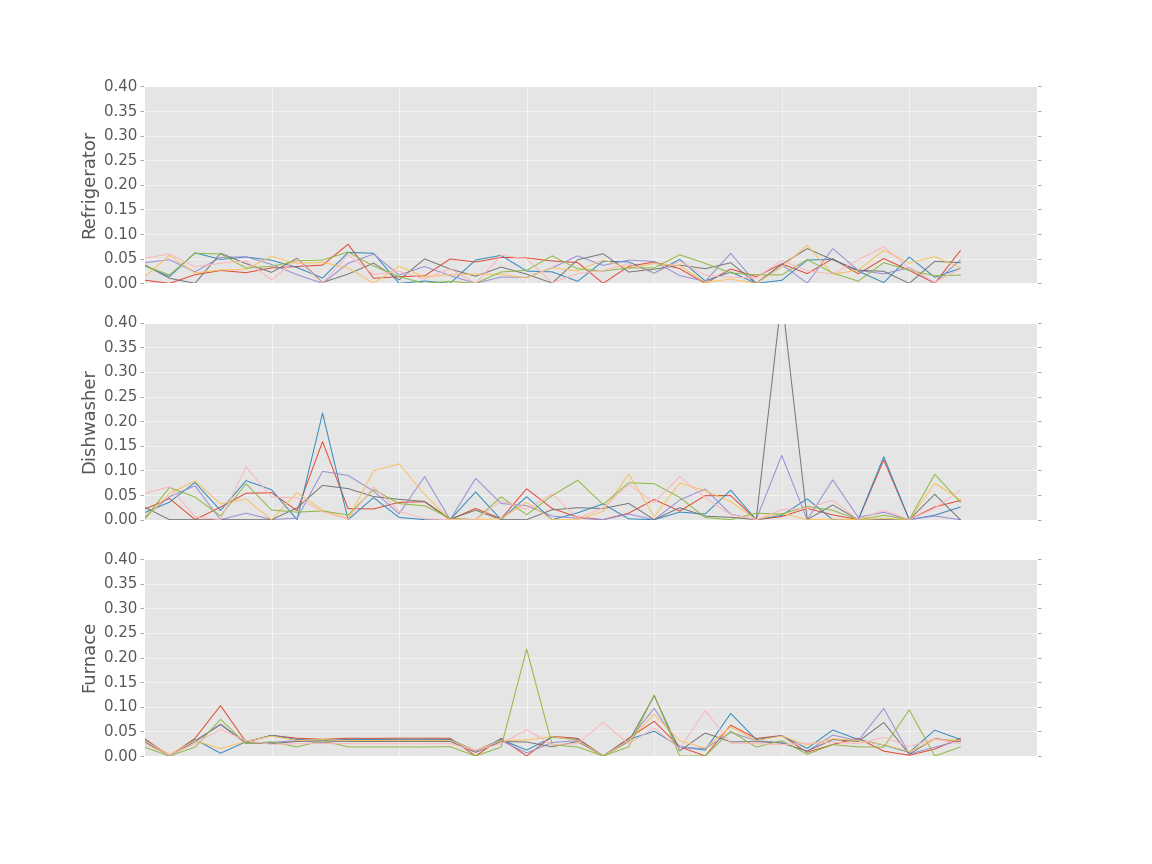
\includegraphics[scale=0.18]{./figures/app_basis}
		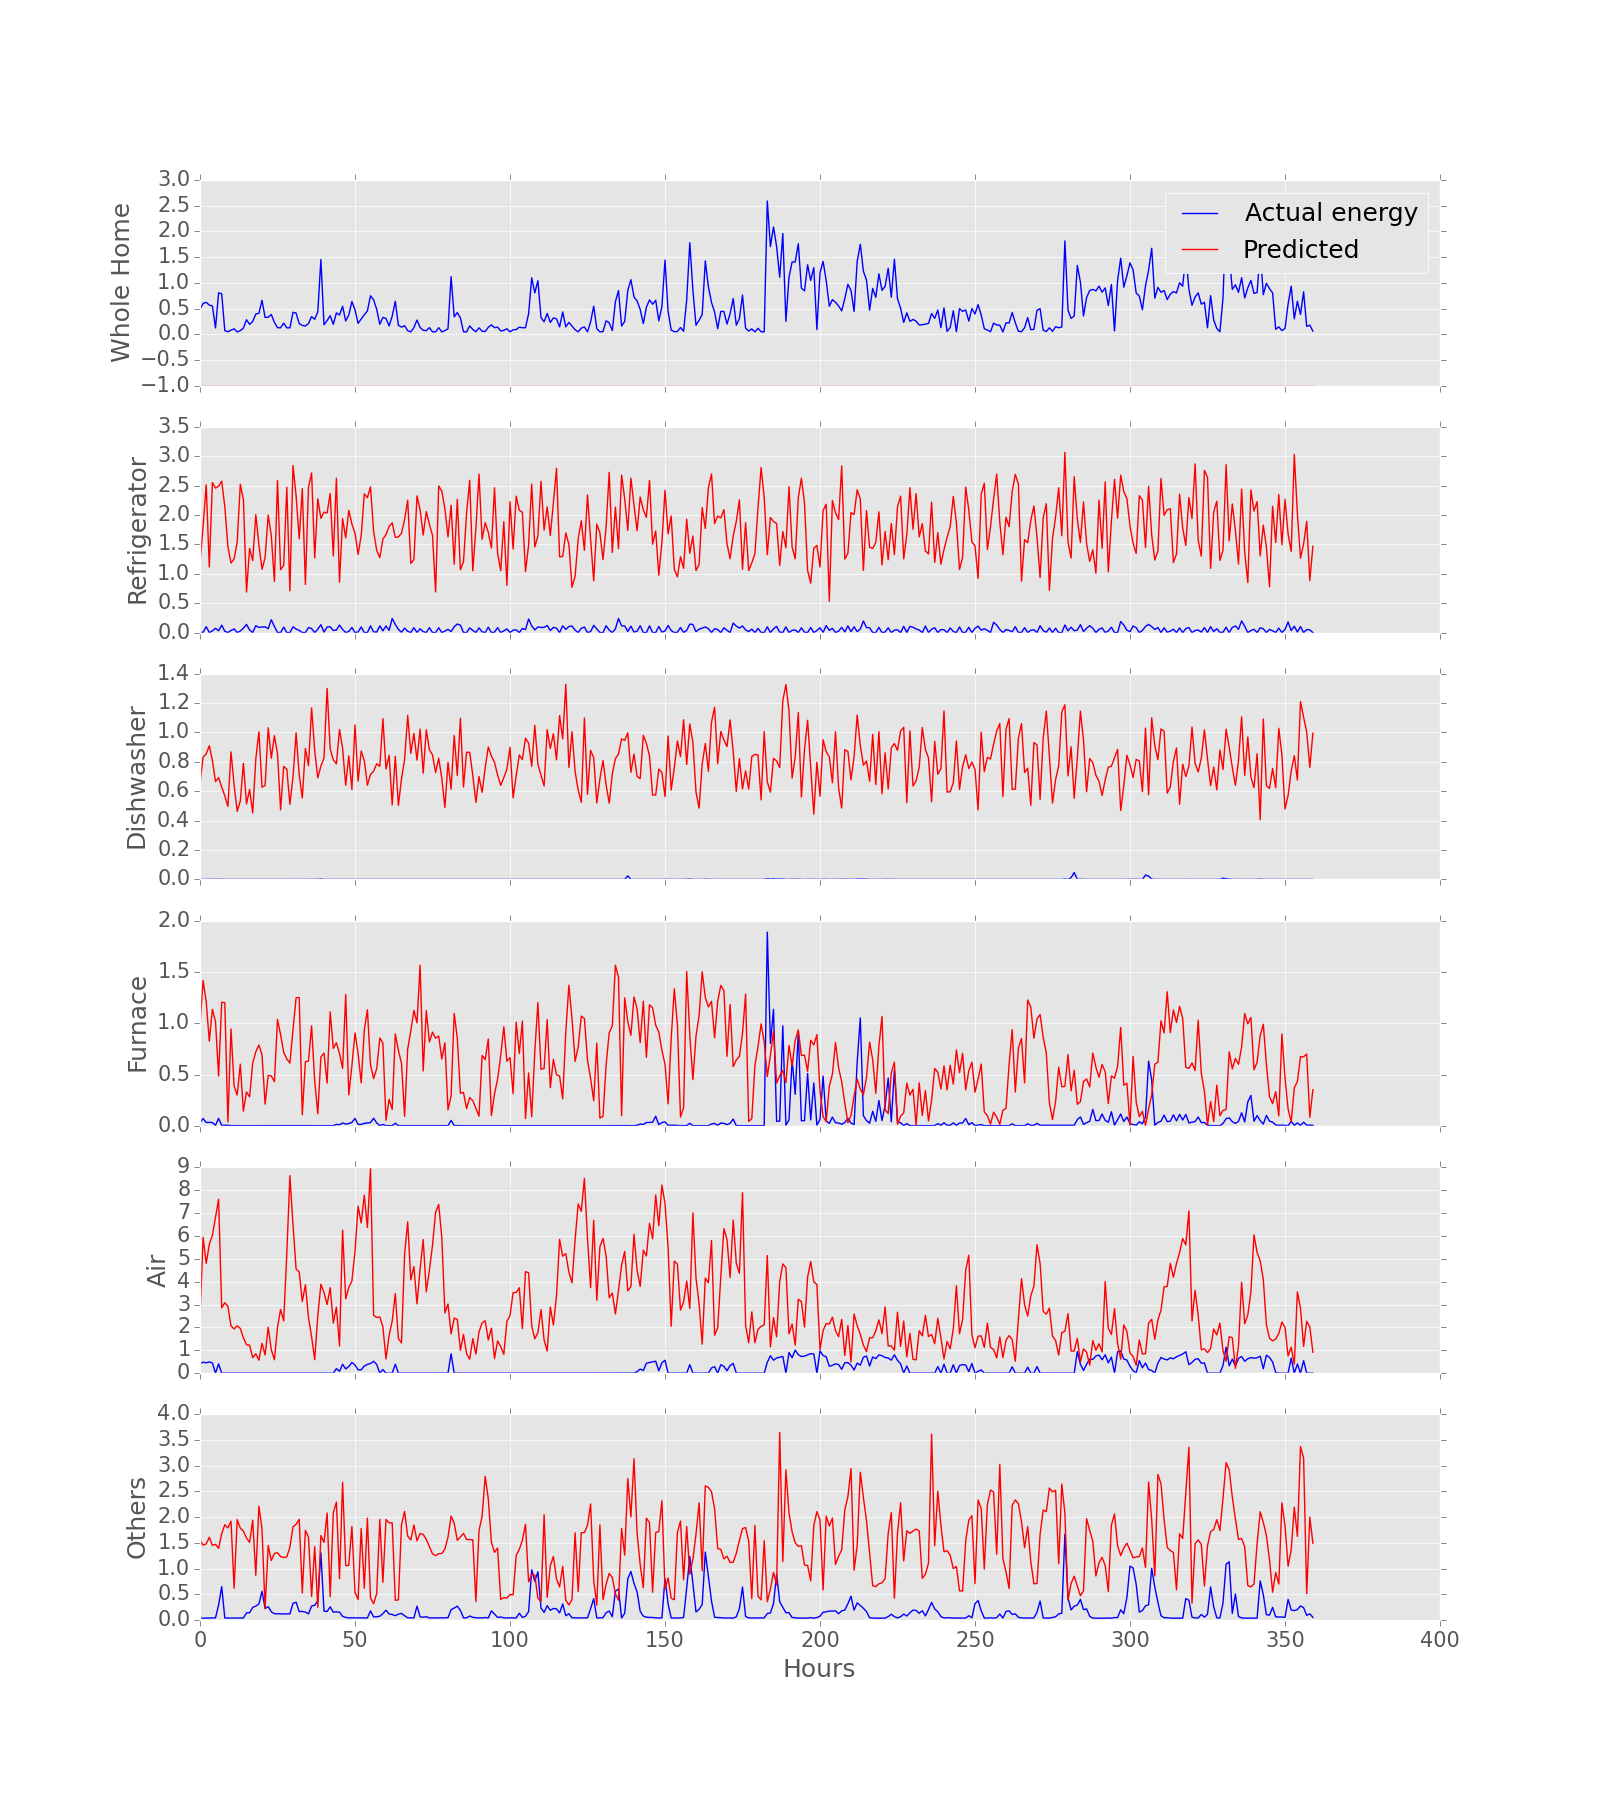
\includegraphics[width=\textwidth,height=10cm]{./figures/results/normal_appliances_144_360}
		\label{fig:test8}
	\end{minipage}%
	\begin{minipage}{.4\textwidth}
		\centering
		%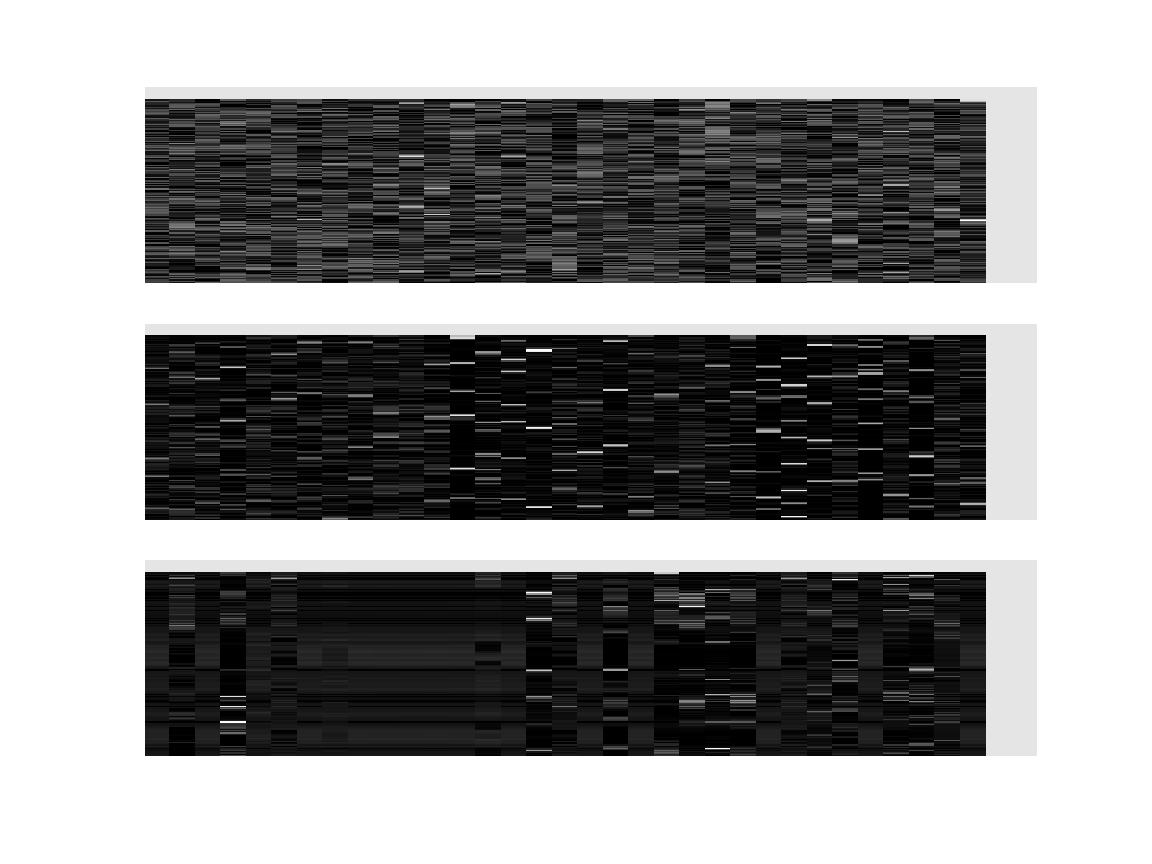
\includegraphics[scale=0.18]{./figures/basis}
		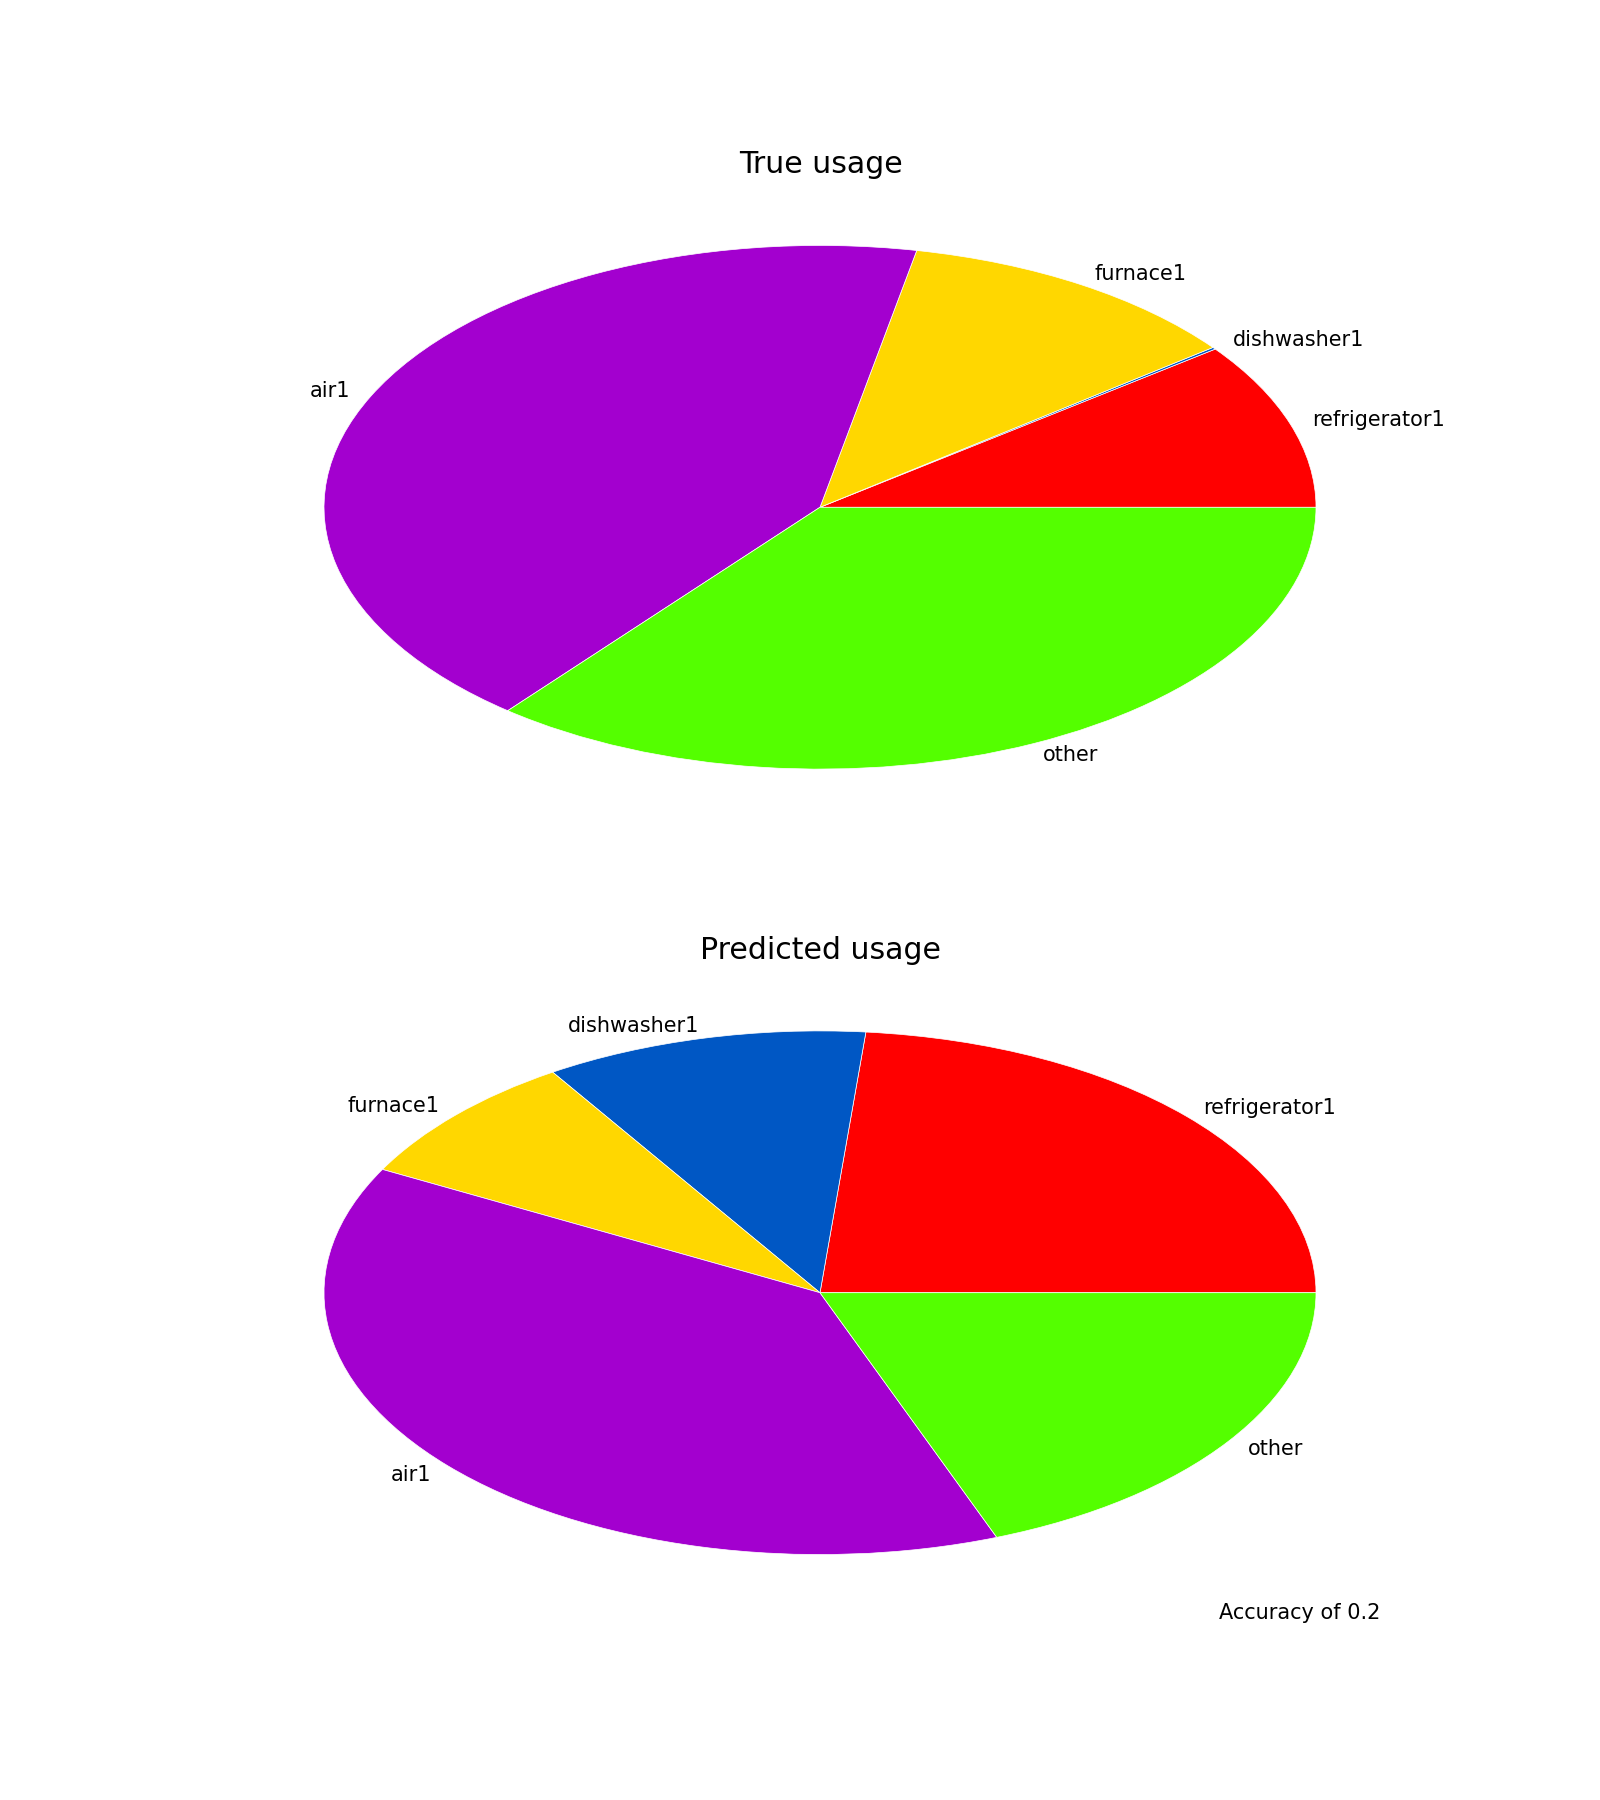
\includegraphics[width=\textwidth,height=10cm]{./figures/results/normal_pie_chart_144_360}
	\end{minipage}
	\caption{Example of one house true energy profile and the predicted energy profile over a two week time period. The plot to the left shows true and predicted energy profiles. The plot to the right shows a piechart of the total percentage that each appliance true usage and predicted usage.}
	\label{fig:normal_360}
\end{figure}

When the algorithm was tested on a two week set of hourly readings, the results were again poor and had a overall accuracy rate of 0.21. The house shows in the plot to the left of the figure \ref{fig:normal_360} has minimal consumption of the dishwasher and refrigerator, but it is visually hard to see as the predicted values are of a magnitude higher. The predicted shapes of the dishwasher and the refrigerator look more or less as a Brownian motion, same as for the prediction of one-week of data but here the predicted values are significantly higher. This behavior could come from the DDSC algorithm where we discriminate the whole signal, and the norm of the activations during this algorithm spikes significantly high, up to 25 000 from a mere 2211, as shown in figure \ref{fig:a_b_ddsc}. This could be that the algorithm overestimates the whole home usage and therefore predicts a higher consumption of the appliances. Furthermore, is that the basis functions are trained to represent the activations trained during this algorithm and that these overestimate some appliances like the dishwasher and the refrigerator seem to have, in both the case for the weekly predictions and of the two week predictions. We can see that all of the appliances are overestimated in their power consumption usage. However, when comparing the predictions for the two tests (week and two weeks) we see that in the later case we see that most of the appliances have been overestimated but in the first case we see that the "other" appliances have been heavily overestimated while both the air and the furnace have been predicted to not be in use at all. This could say that the algorithm can make a better prediction for more appliances when used on a larger dataset. When looking at the pie chart, representing the total percentage use of the predicted versus the true usage, we see from both of the tests, the refrigerator has had the best predicted values. This is probably due to the nature of a refrigerator having a consistent shape, rather than most energy consuming appliance, that have an "on" and "off" behavior.

%% weekdays

\newpage
\subsubsection{Results from weekdays and weekend hourly readings}
\label{sec:days_end}
\begin{figure}[H]
	\centering
	\textbf{168 hours and 67 basis functions \quad 360 hours and 144 basis functions}\par\medskip
	\textbf{Weekday dataset}
	\begin{minipage}{.45\textwidth}
		\centering
		%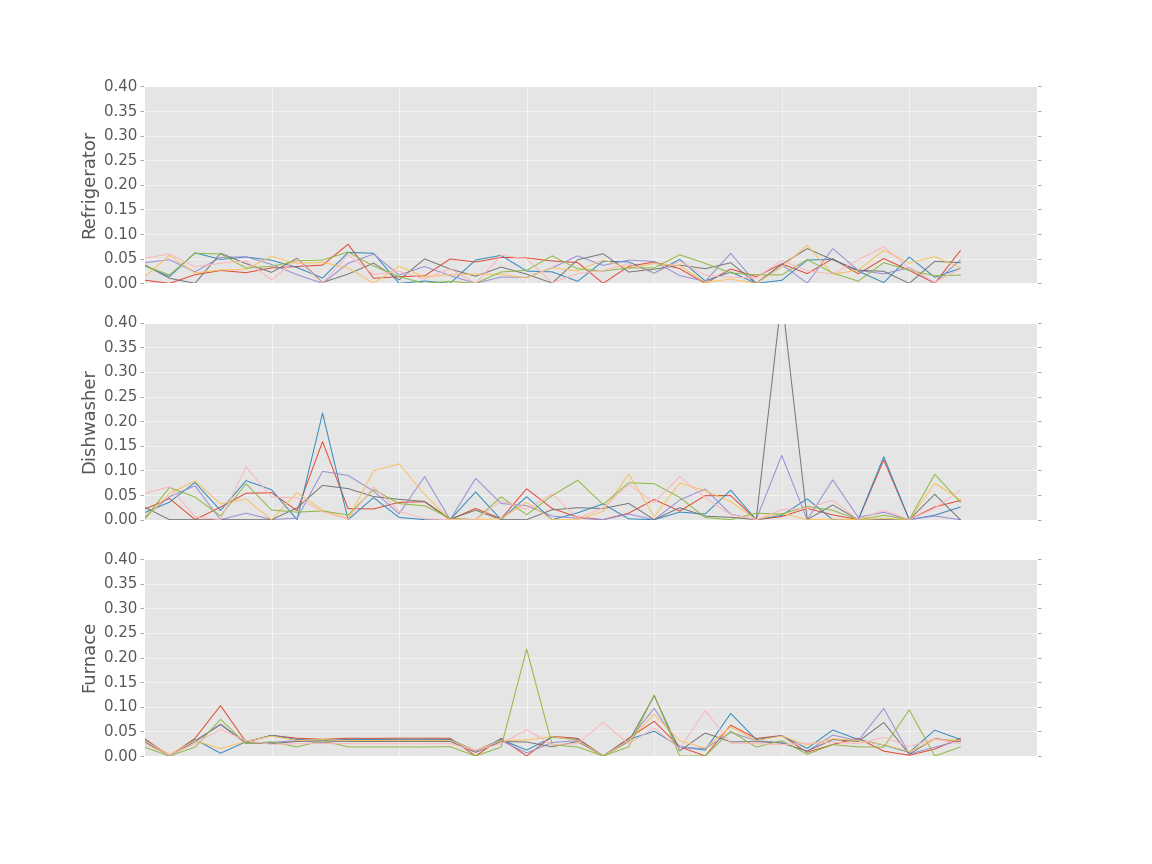
\includegraphics[scale=0.18]{./figures/app_basis}
		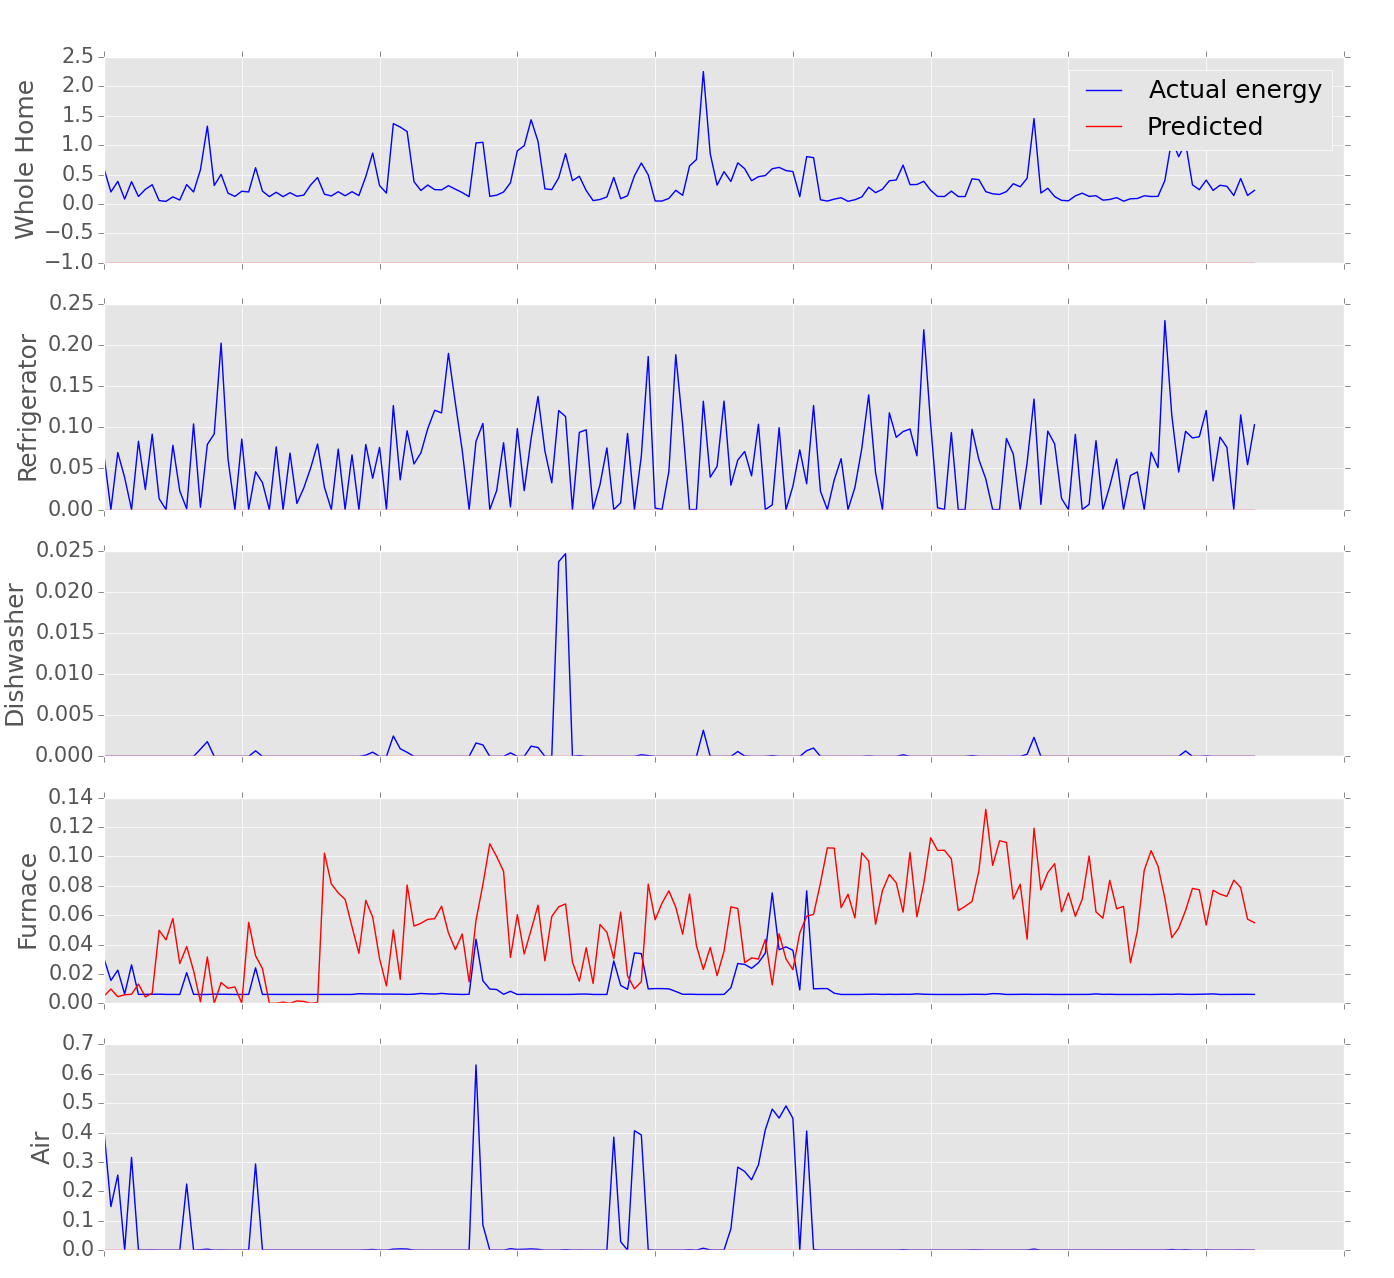
\includegraphics[scale=0.18]{./figures/results/days_appliances_67_168}
	\end{minipage}%
	\begin{minipage}{.45\textwidth}
		\centering
		%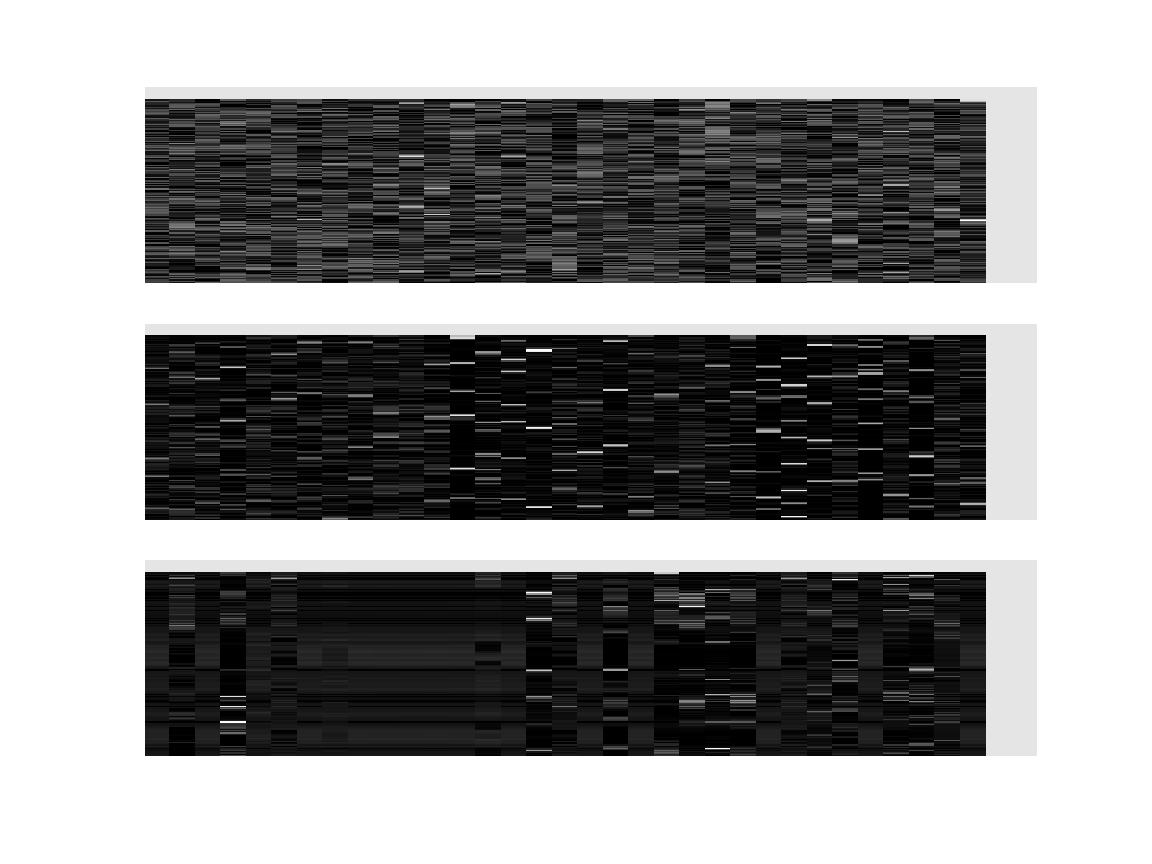
\includegraphics[scale=0.18]{./figures/basis}
		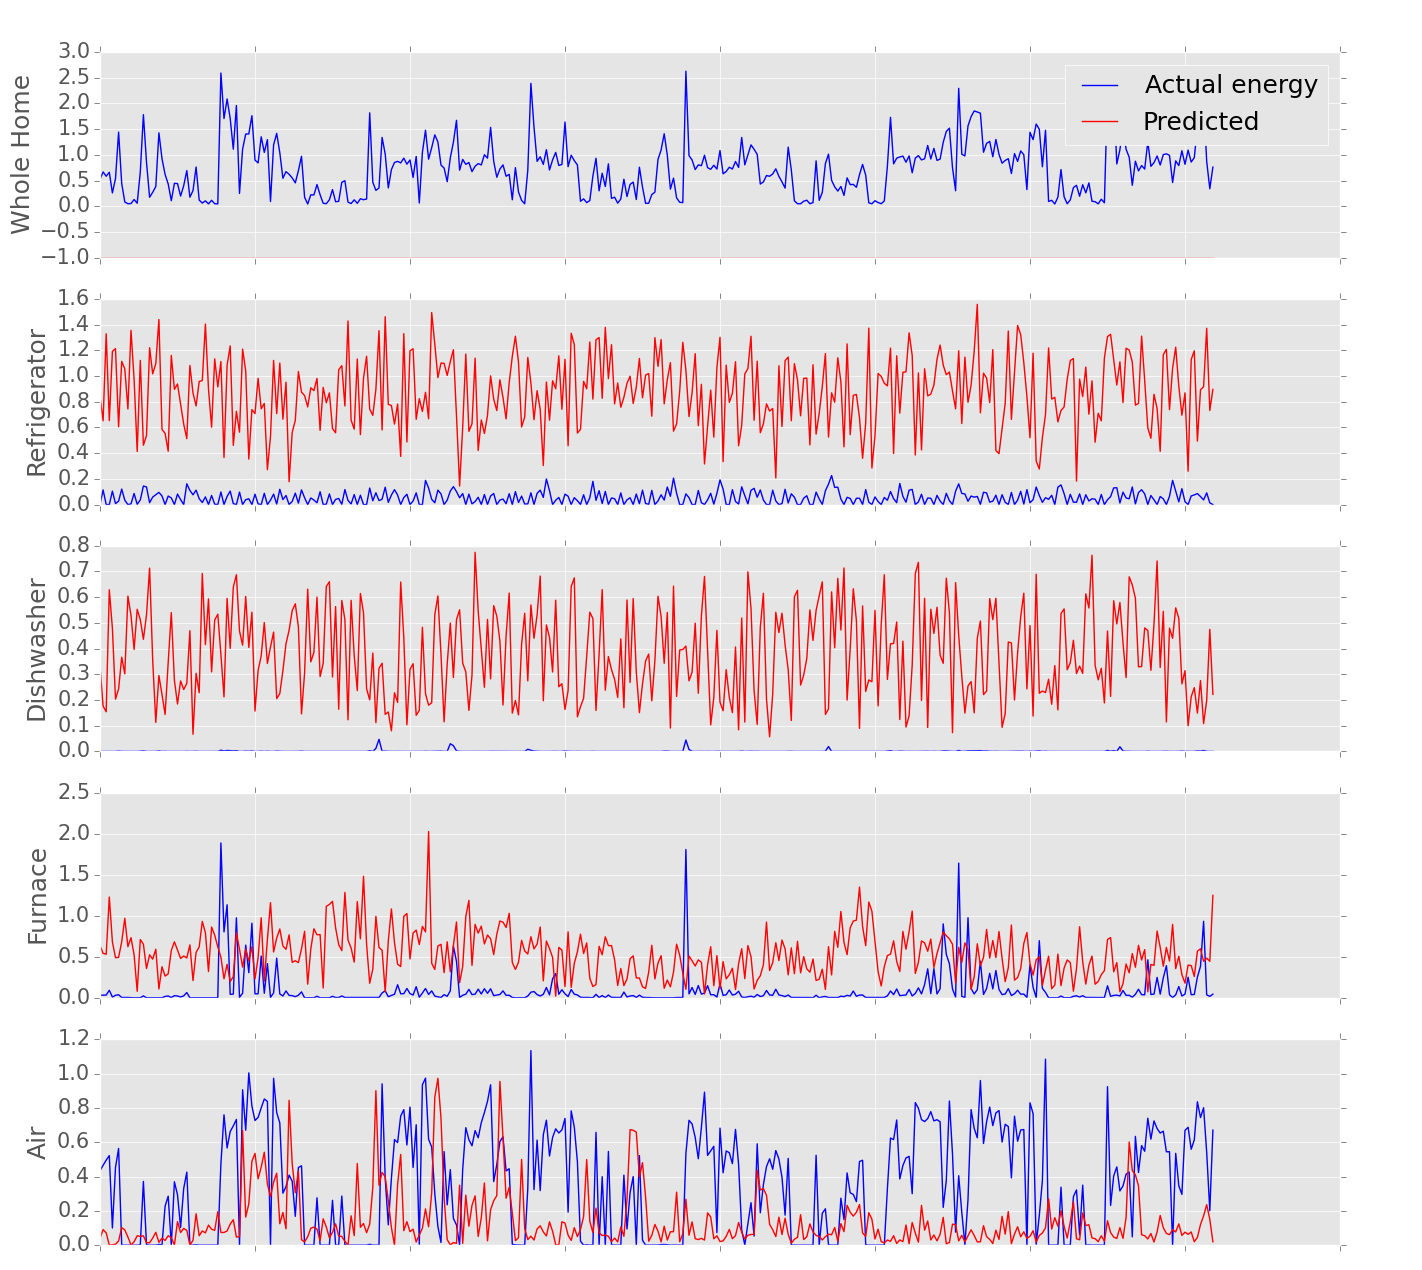
\includegraphics[scale=.18]{./figures/results/days_appliances_144_360}
	\end{minipage}
\end{figure}
%%% weekends
\begin{figure}[H]
	\centering
	\textbf{Weekend dataset}
	\begin{minipage}{.45\textwidth}
		\centering
		%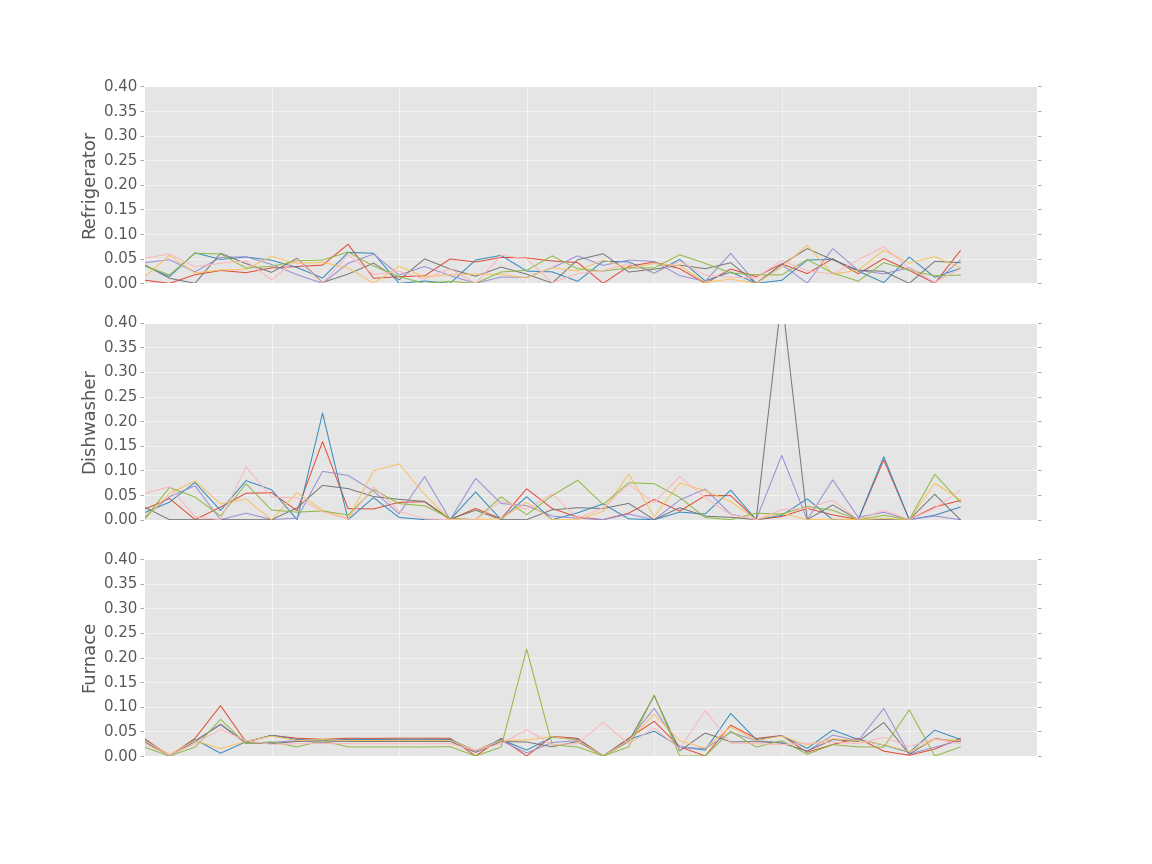
\includegraphics[scale=0.18]{./figures/app_basis}
		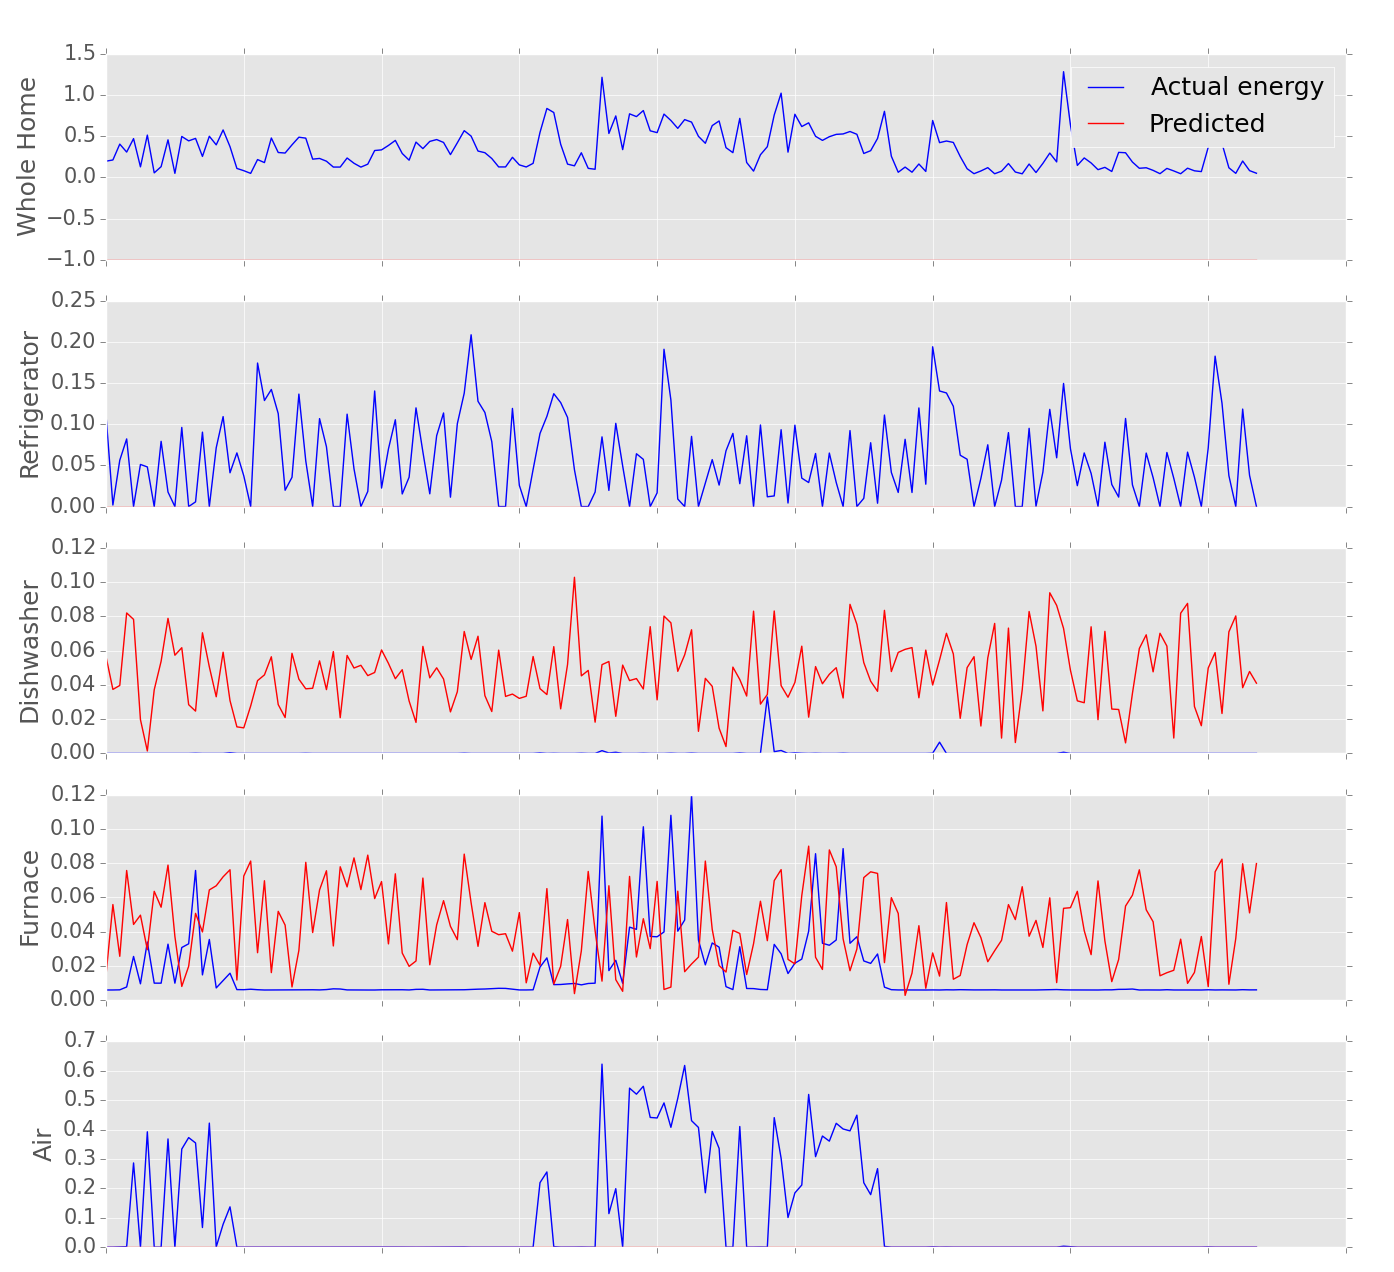
\includegraphics[scale=0.18]{./figures/results/end_appliances_67_168}
	\end{minipage}%
	\begin{minipage}{.45\textwidth}
		\centering
		%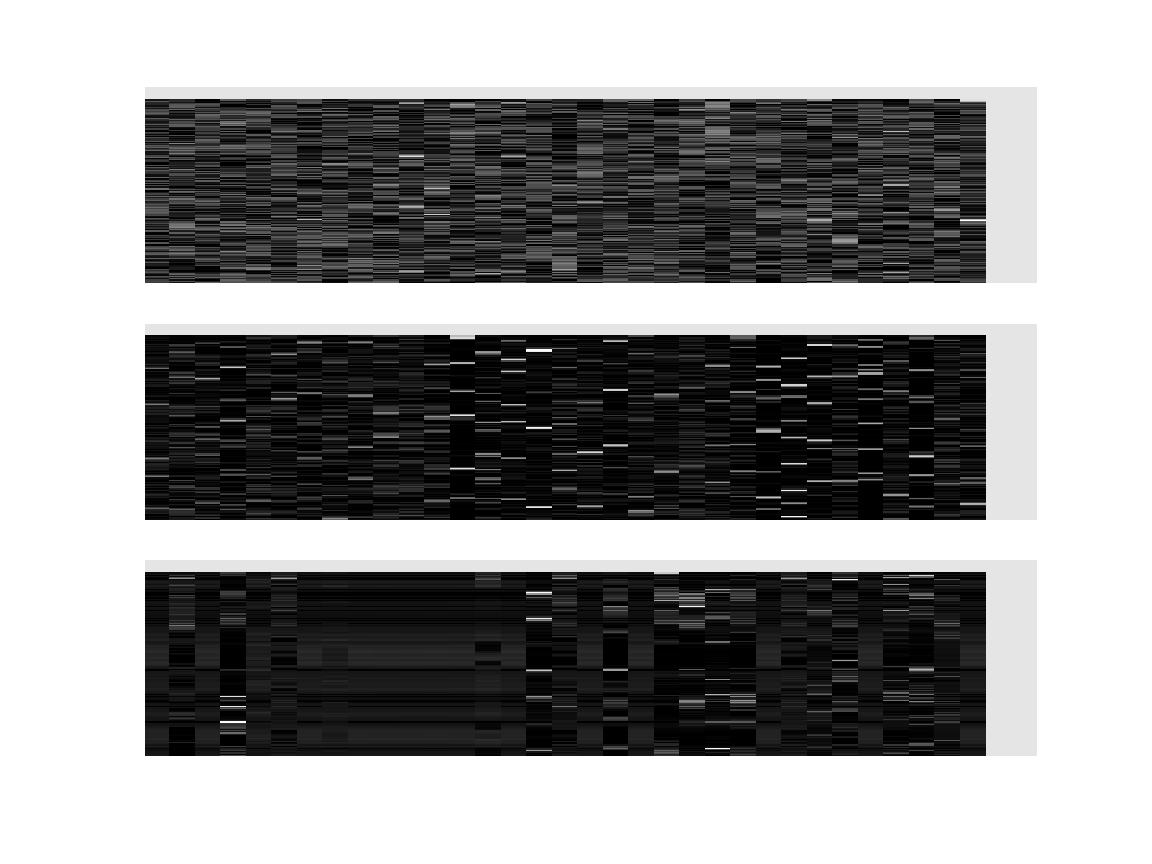
\includegraphics[scale=0.18]{./figures/basis}
		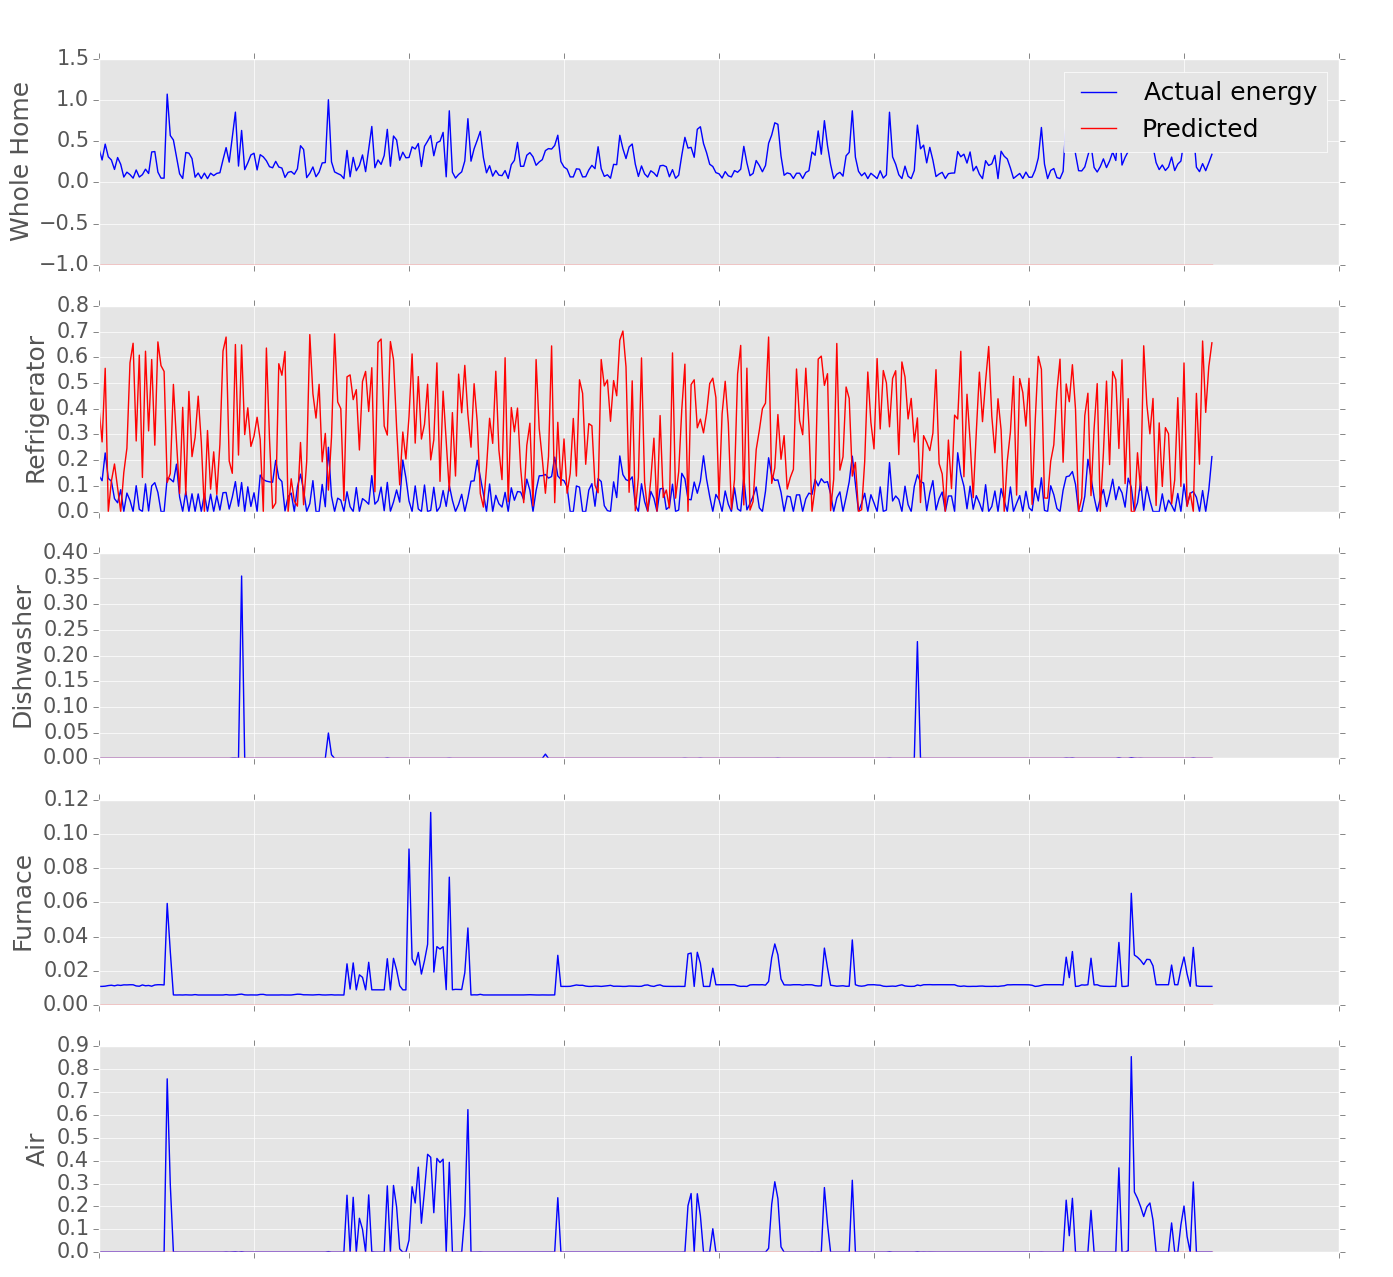
\includegraphics[scale=.18]{./figures/results/end_appliances_144_360}
	\end{minipage}
	\caption{Prediction of the weekday (top plots) and weekend (bottom plots) dataset.}
	\label{fig:days_end}
\end{figure}

The figure \ref{fig:days_end} shows that the predictions have not been successful when it comes to the datasets of weekdays and weekends. It has predicted that only a few appliances use energy. The only successful prediction is the dataset of weekdays for predicting two weeks of consumption. One thing to note is that the prediction of the air-condition for this dataset is the best prediction of all of the tests. It follows the consumption fairly well, and could be a consequence of the usage of air-condition being more homogenous during weekdays than during a whole week. The weekend dataset has the worst prediction of all the datasets, it also preferred to choose one appliance when predicting for two weeks as the week dataset. The prediction failure for the split datasets could be a result of a diminishing of training data, as the splitting of the dataset also made the training set smaller which could be the cause of the bad predictions.

\subsubsection{Basis functions}
\label{sec:a_b}
In addition to the disaggregation results themselves, sparse coding representations of the different device types are interesting in their own right, as they give a good intuition about how the different devices are typically used. The figure \ref{fig:basis_functions} shows a graphical representation of the learned basis functions. In each plot, the gray scale image on the right shows an intensity map of all bases functions learned for that device category, where each column in the image corresponds to a learned basis. 

\begin{figure}[H]
	\begin{center}

	\begin{minipage}{.5\textwidth}
		\centering
		%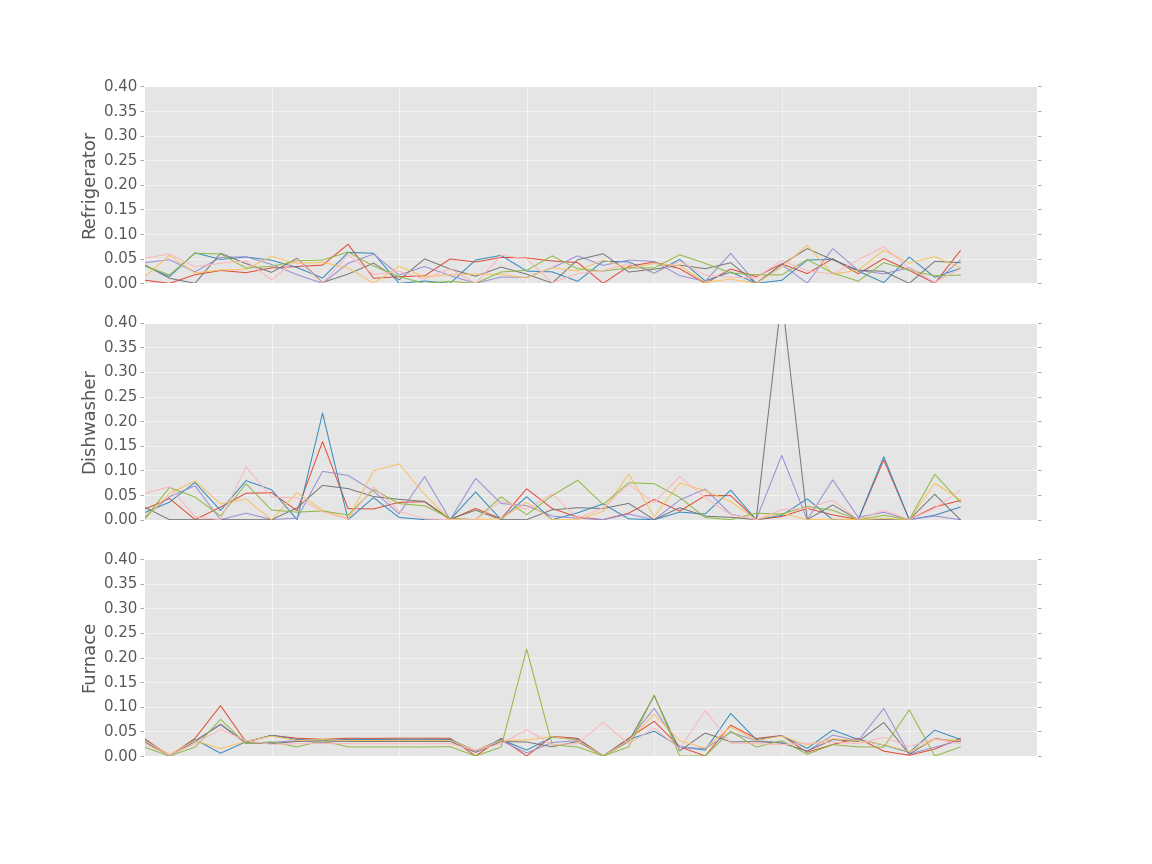
\includegraphics[scale=0.18]{./figures/app_basis}
		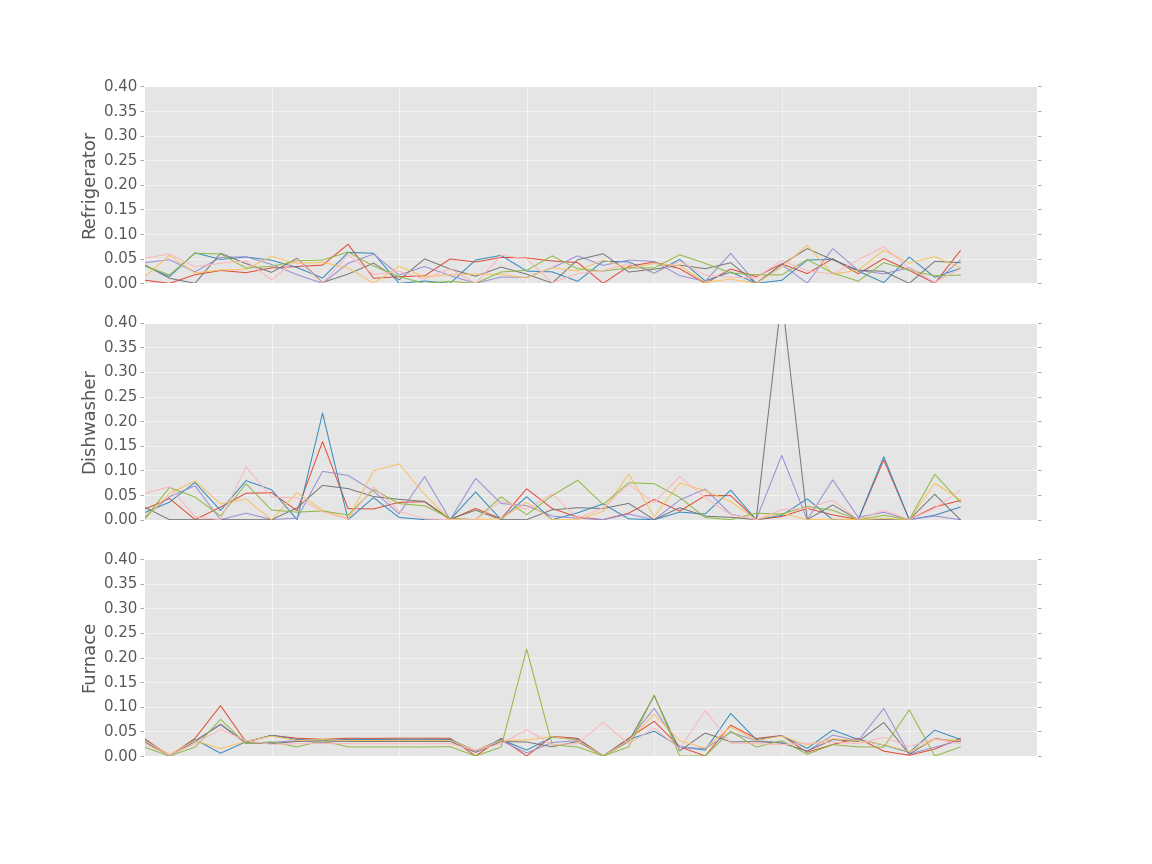
\includegraphics[width=\textwidth,height=12cm]{./figures/app_basis}
		\label{fig:test1}
	\end{minipage}%
	\begin{minipage}{.5\textwidth}
		\centering
		%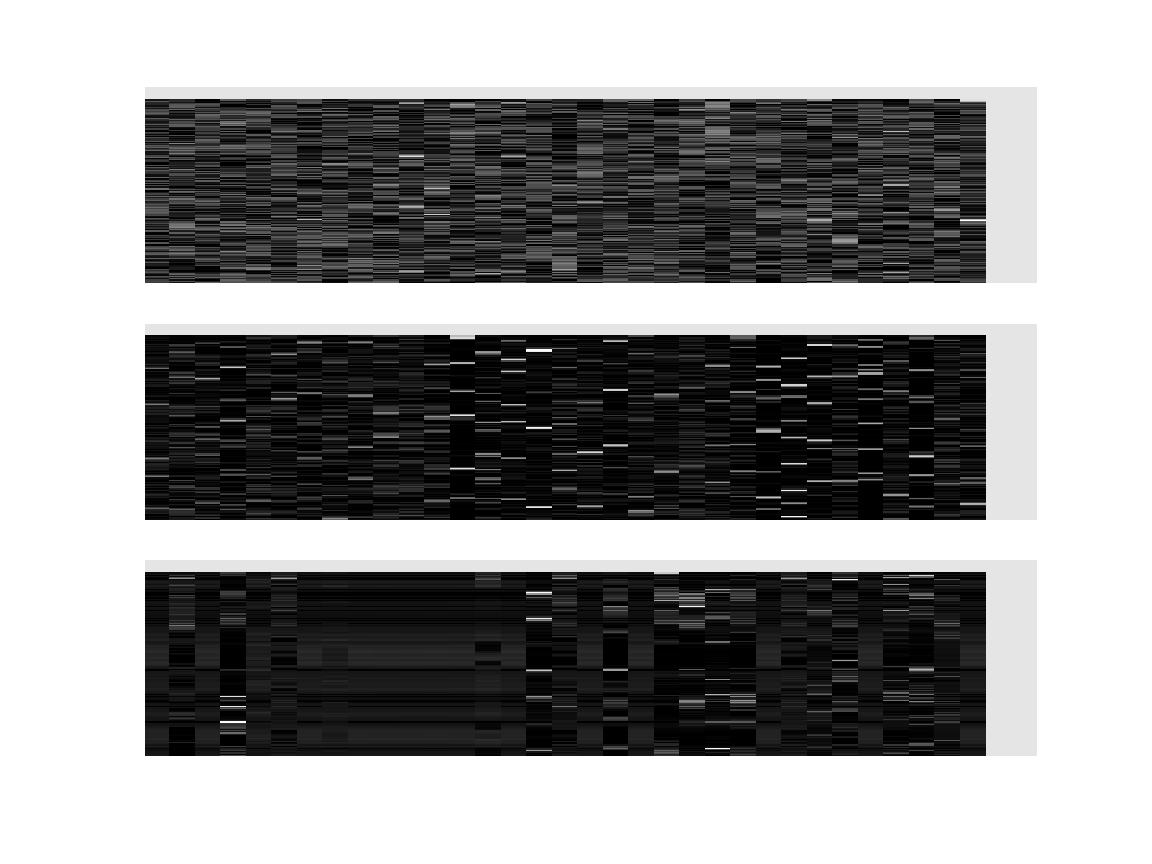
\includegraphics[scale=0.18]{./figures/basis}
		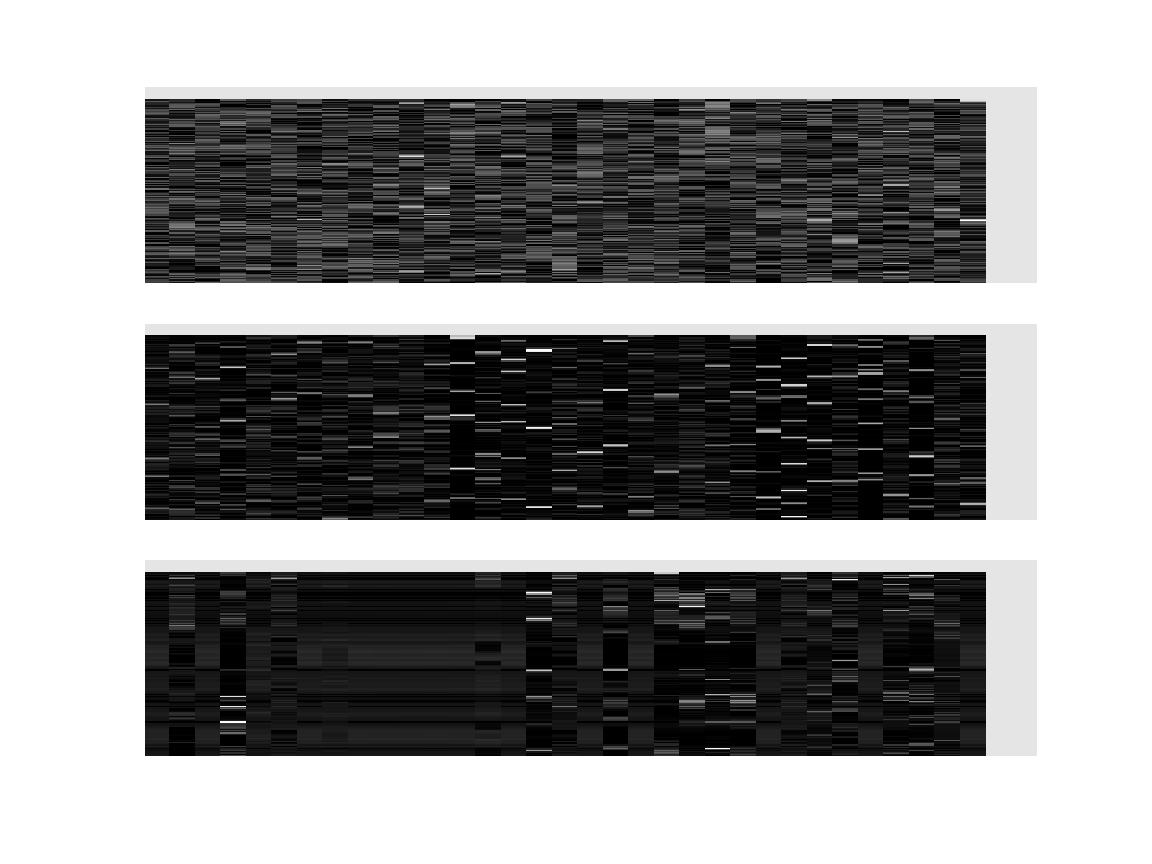
\includegraphics[width=\textwidth,height=12cm]{./figures/basis}
		\label{fig:test2}
	\end{minipage}
	\caption{Example basis functions learned from one device. The plots to the left shows seven example bases, while the image to the right shows all learned basis functions.}
	\label{fig:basis_functions}
	\end{center}
\end{figure}

The plots to the left shows seven examples of basis function for each of the devices. By interpreting the basis functions one can see that refrigerator has a more continuous function applied to it, in contrast to the dishwasher, which has a peak attached to it. This indicates that the functions have captured behaviors, such as "on" and "off" of the refrigerator compared to both the furnace and refrigerator, which in turn we assume do not have "on" and "off" behavior. Kotler et. al. \cite{DDSC} also got basis functions more peaked for refrigerator, which indicate that the basis functions are reasonably representative. They have more heavily peaked functions, which could be from their intense training. It can be said about the furnace, which has some basis that have a peak, which could correspond to a use of the furnace for a temporarily heating of the household. The magnitude of the refrigerator is lower than that of a dishwasher, which says that we have also captured the intensity of power consumption.

The right plots show that the refrigerator is "on" most of the time but with low power as we can see that the plot has mostly grey and some black in it. We can see that the dishwasher has peaked behavior in that some of the basis are almost pure white and some are black. We find interesting behaviors in the representations of the furnace as some of the basis fucntions really do look the same indicating that some furnaces behave similar and in similar magnitude.

\subsection{Quantitative evaluation of the Disaggregation}
\label{sec:quant}

There are a number of components to the final algorithm, and in this section we present quantitative results that evaluate the performance of each of these different algorithms. The most natural metric for evaluating disaggregation performance is the disaggregation error in equation \ref{eq:diserr}, i.e. the overlap of the pie charts of true and predicted percentage energy consumption shown in the figures \ref{fig:normal_168}, \ref{fig:normal_360}. While many of the arguments can be put into the temporal difference, we show that the algorithm has not been able to find a local optimum either by not having a parameter search or training data have not been sufficient. Moreover, the average disaggregation error presented in equation \ref{eq:acc} is not a particularly intuitive metric, and so we also evaluate a total time period accuracy of the prediction system, defined formally as

\begin{equation}
\label{eq:acc}
\text{Accuracy} \vcentcolon=  \frac{\sum_{i,q} \min \left\{ \sum_p ( \mathbf{X}_i)_{pq}, \sum_p ( \mathbf{B}_i,\hat{\mathbf{A}}_i)_{pq} \right\}}{\sum_{p,q} \bar{\mathbf{X}_i}_{p,q}}
\end{equation}

Despite the complex definition, this quantity simply captures the average amount of energy predicted correctly over the time period (i.e., the overlap between the actual and predicted energy).

\begin{figure}[H]
	\centering
	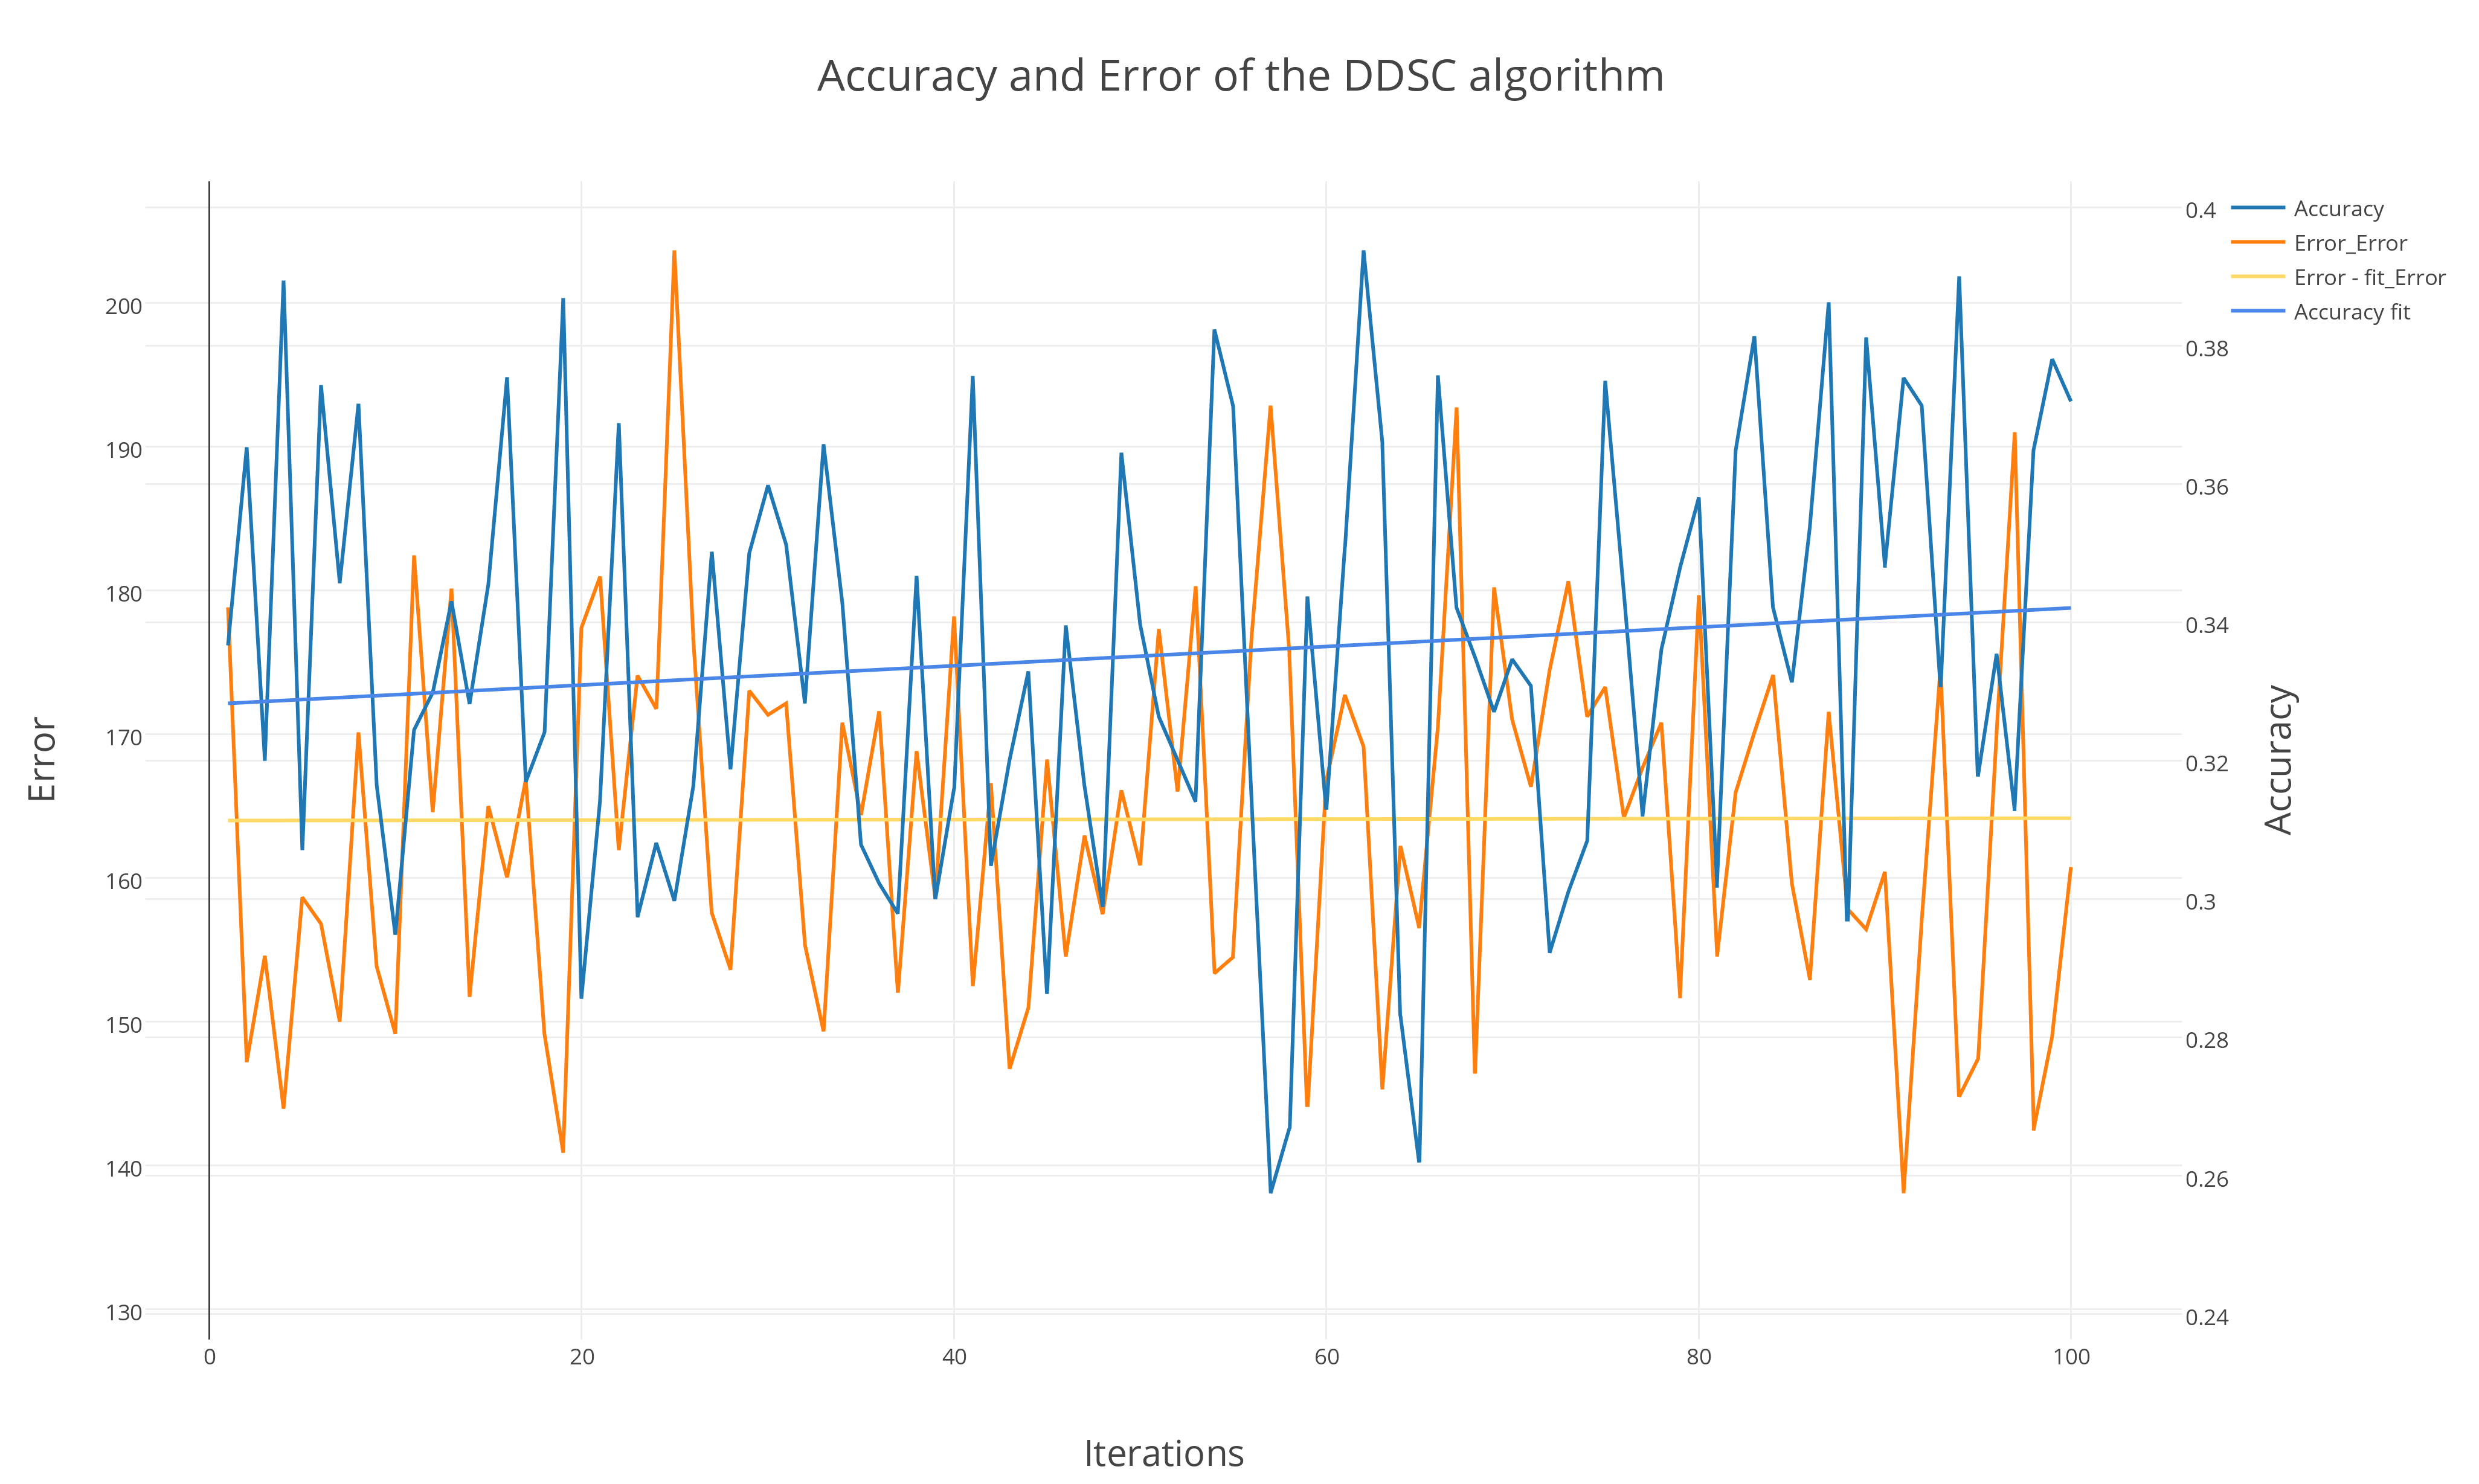
\includegraphics[scale=0.45]{./figures/acc_err_ddsc}
	\caption{Evolution of the training accuracy and error for the DDSC updates. The figure shows the best prediction of all the runs of the algorithm.}
	\label{fig:acc_err_ddsc}
\end{figure}

Figure \ref{fig:acc_err_ddsc} shows the disaggregation performance for the DDSC algorithm \ref{alg:ddsc}. It presents the disaggregation error from equation \ref{eq:diserr} on the left y-axis and the accuracy given in equation \ref{eq:acc} on the right y-axis. Furthermore a linear regression has been done for both the error and accuracy. We note that the accuracy is around 35\% following the fitted line when the 100:th iteration has been done. From the figure we see that for each iteration, the algorithm has difficulty finding an optimal path towards a minimization as seen by the volatile behavior of both the error and accuracy. However, fitting a curve to the values, we see that the accuracy has a positive slope although with regards to a high variance for curve fitting, the plot shows that we cannot fully rely on the implementation due to its behavior. Investigating this further, we took a look at the activation and basis norms of the algorithm. This yielded the following figure.

\begin{figure}[H]

	\centering
	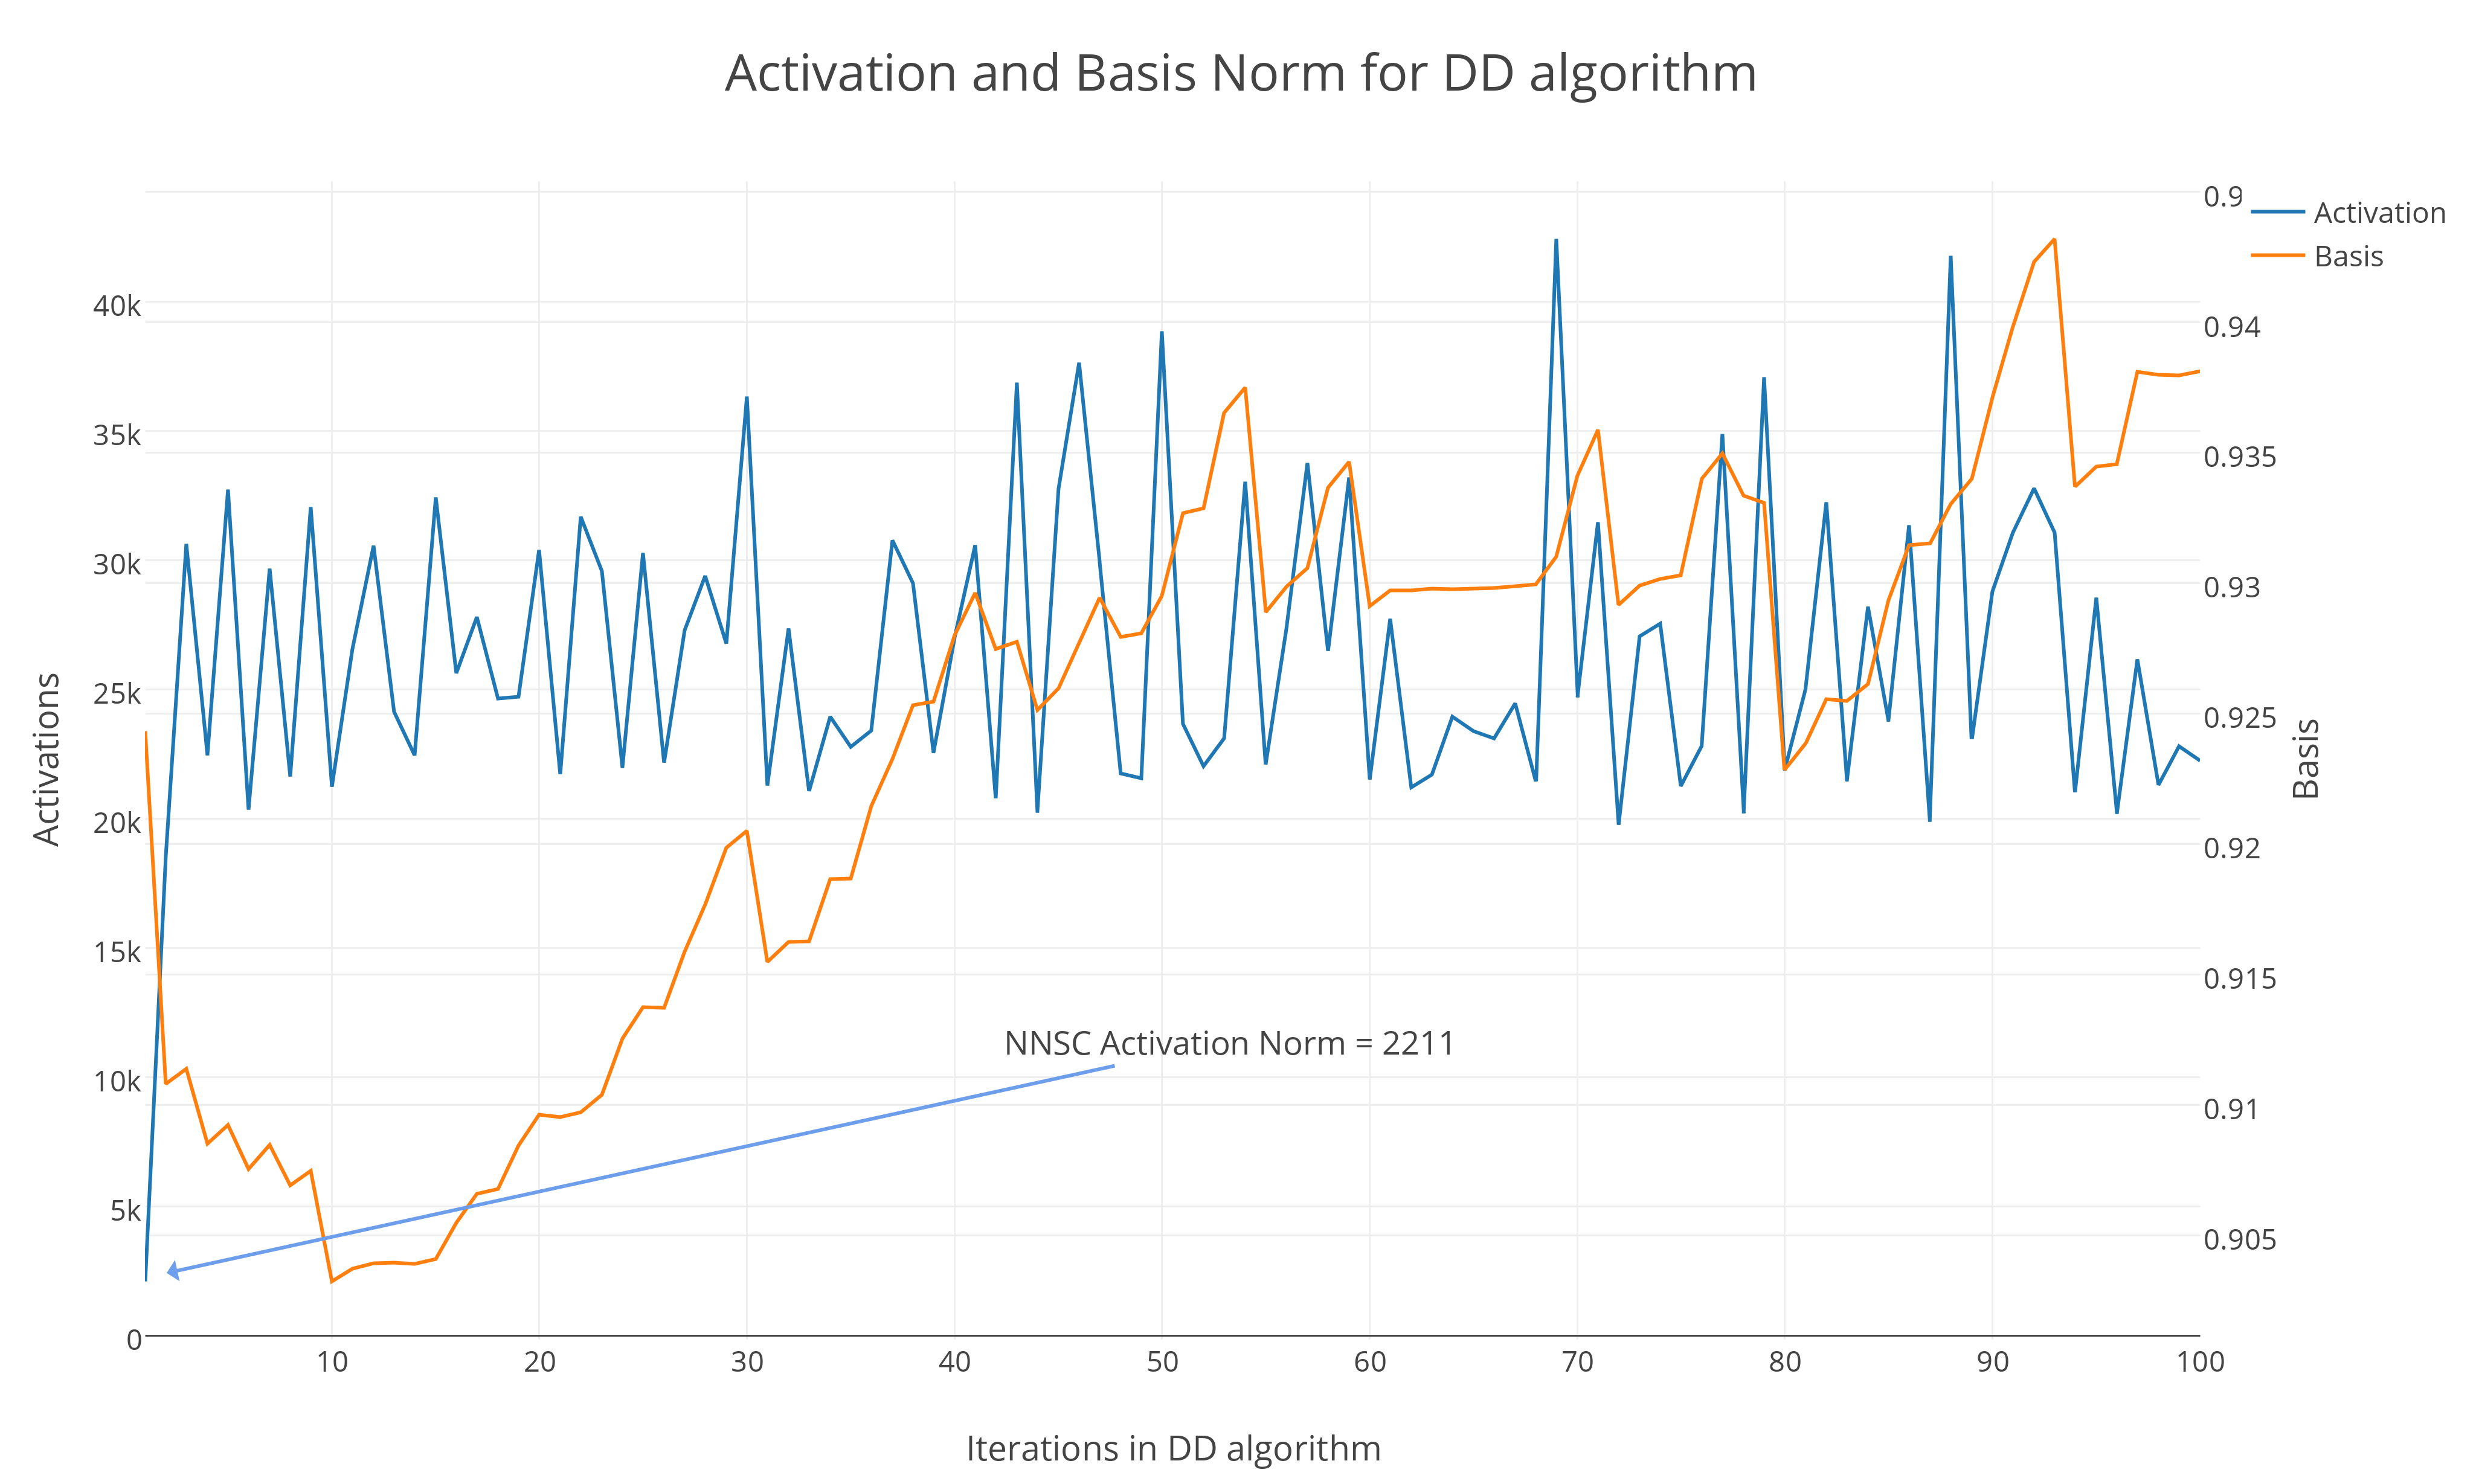
\includegraphics[scale=0.45]{./figures/a_b_norm}
	\caption{Evolution of the Activation and Basis norms for the DDSC updates. The norm of the Activations are seen on the left y-axis and the left y-axis is the Basis norm.}
	\label{fig:a_b_ddsc}
\end{figure}

The NNSC algorithm trains its activations separately for all of the appliances and yielded a norm of 2211 cumulatively for all of the appliances. We can see from the plot that when we start the DDSC algorithm the activation norms go from 2211 to around 25 000, which is probably due to the activations trying to adapt to the whole home energy consumption, which is vastly larger than each appliance. Interesting to note is that the basis norm slightly increases with each iteration, while the activations oscillate around 25 000. The activations trained are not used for the predicting the values for a new dataset, from this iteration we only take out the basis matrix which seems to have adapted itself by changing from a norm of 0.925 to 0.94.


\newpage
\section{Conclusions and Open Questions}
%• Conclusions/discussion: Did we reach the result we were aiming for? If not why?
%Would another approach have been better? What significance does the results have?
%What would be an appropriate next step?
This section discusses and concludes the results from section \ref{sec:evaluation} given by this paper, in sections \ref{sec:results}-\ref{sec:temp}. We also present future research and improvements in section \ref{sec:future}.

\subsection{Energy Disaggregation results}
\label{sec:results}
The disaggregation algorithm has shown to be implemented correctly but used with caution with regards to data, parameters and computational power. The algorithm has an overall accuracy of around 25\% by the equation \ref{eq:acc}. This would however say that we have a good accuracy compared to what the energy profiles show in the figures in section \ref{sec:evaluation}. Most of the predicted energy profiles for larger datasets are heavily overestimated in their energy consumption. Moreover, the results for a week and two weeks have shown not to provide accurate results given that we use lesser basis functions than the models suggest. They might be improved by providing the algorithm with computational power and thereby use sufficient basis functions as shown in the results in the beginning of section \ref{sec:evaluation}. Here we used roughly 10 times the amount of basis functions compared to the dimensions of the data, which provided more accurate results. The algorithm can surely be improved with computational power by providing the algorithm with more samples (houses), in the results provided in this thesis we had to even cut a good amount of good data to be able to run the algorithm, the dataset that Pecan Street \cite{pecan} really provided, was an extensive amount of data, we discuss more on that in section \ref{sec:dataset}.

The algorithm shown to be good at producing complex structures, such as a dishwasher being "on" and "off" during a certain time period, as shown in the figures for the basis functions \ref{fig:basis_functions}, it can also be shown in the prediction for the air-condition in figure \ref{fig:subset}. However, it was not accurate at which of the appliances that were being used, the algorithm seemed to infer that one appliance stood for most of the energy consumption, which was false for most of the data. It also highly overestimated the power consumption of all of the appliances. This could be a fault in the DDSC algorithm implemented as shown in the evaluation of the norms during the training. The norm of the activations seemed to react heavily for the whole home energy usage and might have provided the algorithm with an overestimation of the energy consumption for all of the appliances.

\subsection{Algorithm}

The algorithm provided in Kotler et.al in \cite{DDSC} was cumbersome to implement. They provide a section with model implementation but state that they have precluded the details due to space constraints. Thankfully Scikit-learn \cite{scikit} has been a source to go to for help regarding implementing such an algorithm, such as the DDSC. The algorithm also has some parameter choices, which was fitted using grid-search, this was however not implemented and could provide the algorithm with better results. They did not state explicitly which parameters they used for disaggregation which would have made the implementation easier, see section \ref{sec:params} below for more thought on the parameters for the algorithm. The overestimation of the energy consumption might have been avoided by implementing the extension presented below in section \ref{sec:extensions}.

\subsubsection{Extensions}
\label{sec:extensions}
Here we present the extension proposed by Kotler et.al. \cite{DDSC} to modify the standard Sparse Coding formulation. This could be implemented into the model, which was said to increase accuracy by 1.3\% when using both of the extensions, more detail explanations are in their paper \cite{DDSC} page five.

\textbf{Total energy priors.} Kotler et. al. mention that the Sparse Coding model presented does not take into consideration the different power consumptions that the appliances might have. They could take similar shapes such as dishwasher and refrigerator into the same category while they might have totally different power consumption while operating. In summary, this extension penalizes the deviation between a device and its mean total energy. \cite{DDSC}
\vspace{0.1in}
\[
F_{TEP}(\bar{\mathbf{X}},\mathbf{B}_{1:k},\mathbf{A}_{1:k}) = F(\bar{\mathbf{X}},\mathbf{B}_{1:k} \mathbf{A}_{1:k}) + \lambda_{TEP}\sum_{i=1}^k \norm{\mu_i\mathbf{1}^T-\mathbf{1}^T\mathbf{B}_i\mathbf{A}_i}^2_2
\]
where $\mathbf{1}$ denotes a vector of ones of the appropriate size, and $\mu_i = \frac{1}{m} \mathbf{1}^T \mathbf{X}_i$ denotes the average total energy of device class $i$.
\vspace{0.1in}
\\
\textbf{Group Lasso.} Since energy consumption exhibit some sparsity at the device level (zero energy consumption, or not being monitored in the home), Kotler et.al. encourage a grouping effect to the activations. This could have prevented the algorithm for prioritizing one appliance across all of the other appliances. To achieve extension, one can employ the group Lasso algorithm \cite{grouplasso}, 
\vspace{0.1in}
\[
F_{GL}(\bar{\mathbf{X}},\mathbf{B}_{1:k},\mathbf{A}_{1:k}) = F(\bar{\mathbf{X}},\mathbf{B}_{1:k} \mathbf{A}_{1:k}) + \lambda_{GL}\sum_{i=1}^k \sum_{j=1}^m \norm{\mathbf{a}_i^{(j)}}_2
\]
They also present \textbf{Shift Invariant Sparse Coding}, which they say could not capture the information wanted. \cite{DDSC}

\subsection{Dataset}
\label{sec:dataset}

The dataset needed a lot of preparation to be able to even come remotely close to being a full dataset. Kotler et.al. did not address if they spent time on data pre-processing any of the data which seems almost unreasonable for their amount of data. Furthermore, the assumptions made in the data pre-processing for this thesis, presented in detail in section \ref{sec:prep} have made an impact on the results and Kotler et.al. do not present any of these assumptions that must have been made to be able to work with that amount of data. The dataset used in this thesis has not been validated via a cross-validation, which could improve the algorithm slightly.
In this thesis data from the Pecan Street was shown to represent a Weibull distribution which could be used for a generalization of the energy consumption in the area around Pecan Street or used for disaggregation based on distributional disaggregation, such as Semi-Markov models \cite{kotler2}.

%\pagebreak[3]
\subsection{Temporal difference}
\label{sec:temp}
This thesis has shown that trying to train the algorithm by exploiting temporal difference has not been proven useful. The conclusion drawn from this is that one should use, as much data as available as Sparse Coding needs enough data for it to provide a good representation of the profiles. Training data for other appliances other than that of Pecan Street are scarce and hard to come by, which indicates that we need to use the data that is available.

\subsection{Future research}
\label{sec:future}
Here we present future research that might come to help with DDSC algorithm or provide insight into the field of energy disaggregation as a whole.
\subsubsection{Hyper-parameter Optimization}
\label{sec:params}

The type of hyper-parameter controls the capacity of a model, i.e., how flexible the model is, how many degrees of freedom it has in fitting the data. Proper control of model capacity can prevent overfitting, which happens when the model is too flexible, and the training process adapts too much to the training data, thereby losing predictive accuracy on new test data. So a proper setting of the hyper-parameters is important \cite{hyper}.

There exists algorithms for defining the hyper-parameters of the model, one being that of Sequential Model-based Global Optimization (SMBO). These algorithms have been used in applications where evaluation of the fitness function is expensive. In an application where the true fitness function $f : X \rightarrow R$ is costly to evaluate, model-based algorithms approximate $f$ with a surrogate
that is cheaper to evaluate \cite{hyper}. There also exits "The Gaussian Process Approach", Tree-structured Parzen Estimator Approach (TPE), Random Search for Hyper-Parameter Optimization in DBNs (deep-belief-networks) and Sequential Search for Hyper-Parameter Optimization in DBNs. The latter of the two could prove to be valuable for methods just like the DDSC algorithm for providing the algorithm with the correct hyper-parameters for the model \cite{hyper}.

\subsubsection{Autoencoders}

Most Deep Learning systems heavily use unlabeled as well as labeled data. Large amounts of unlabeled data (Millions of pictures, gigabytes of text, tons of hours of voice) are used for feature learning mainly through deep autoencoders. The output of this phase is a high level abstraction of the data. The recent development with using autoencoders by Google in 2012, where even Andrew Yg. contributed to the work. There an unsupervised deep learning approach was used, trained it with Millions of YouTube images and the final neurons could recognize faces, cars, and cats. So for this network you just need to map the neurons to the labels you like to have, e.g. this is a face, a car, a cat. \cite{google} The large amount of unlabeled data that makes up the energy sector makes deep learning approaches so strong.

\subsubsection{Block Coordinate Update}
\label{sec:bcd}
Regularized block multiconvex optimization presented in 2013 by Yangyang Xu and Wotao Yin \cite{block2}, is an interesting approach, where the feasible set and objective function are generally non-convex but convex in each block of variables. It also accepts non-convex blocks and requires these blocks to be updated by proximal minimization. Compared to the existing state-of-the-art algorithms, the proposed algorithm demonstrate superior performance in both speed and solution quality. This work could pose to be the next approach to energy disaggregation.

\subsubsection{Dropout}
Dropout, by Hinton et al. \cite{dropout}, in 2014, is perhaps the biggest invention in the field of neural networks in recent years. It addresses the main problem in machine learning that is overfitting. It does so by “dropping out” some unit activations in a given layer that is setting them to zero. Thus it prevents co-adaptation of units and can also be seen as a method of assembling many networks sharing the same weights. For each training example a different set of units to drop is randomly chosen. The dropout procedure can also be applied to the input layer by randomly deleting some of the input-vector components typically an input component is deleted with a smaller probability. Dropout has been reported to yield remarkable improvements on several difficult problems, for instance in speech and image recognition and hopefully could provide a means to remove overfitting in energy disaggregation as well. \cite{dropout}

\subsection{Final words, Open questions}
One interesting take that was discussed during this thesis was the precision of the algorithms for energy disaggregation. If we would be able to disaggregate with an accuracy of over 90\%, how would the public react with privacy issues? Would people want to provide their energy usage and if so, how much can be attained by the utility companies?
\newpage

%\section{Bibliography}
\begin{thebibliography}{9}

\bibitem{lip}
 M. H. Albert, R. J. Nowakowski, D. Wolfe,
 \emph{Lessons in Play: An Introduction to Combinatorial Game Theory.}
 Wellesley, Massachusetts:
 A K Peters, Ltd;
 2007.
  
\bibitem{bouton1901}
  C. L. Bouton, 
  \emph{Nim, A Game with a Complete Mathematical Theory.} 
  In: The Annals of Mathematics;
  2nd Ser., Vol. 3, No. 1/4,
  1901.
  p. 35–39.

\bibitem{onag}
  J. H. Conway,
  \emph{On Numbers and Games}.
  2nd ed.
  London:
  Academic Press;
  1976.
  
\bibitem{grier2013}
  D. Grier, 
  \emph{Deciding the Winner of an Arbitrary Finite Poset Game Is PSPACE-Complete.} 
  In: F. V. Fomin, R. Freivalds, M. Z. Kwiatkowska, D. Peleg, editors. 
  ICALP(1) 2013;
  2013 Jul 8-12;
  Riga, Latvia.
  Berlin, Germany: 
  Springer Berlin Heidelberg;
  2013. 
  p. 497–503.

%\bibitem{hk2002}
% J. Hong, S. J. Kang,
% \emph{Introduction to Quantum Groups and Crystal Bases.}
% Graduate Studies in Mathematics.
% Volume 42.
% American Mathematical Society;
% 2002.

\bibitem{j2013}
 E. J\"arleberg,
 \emph{Pomax Games: A New Class of Partizan Games Played On Posets.}
 Master’s Thesis.
 Stockholm:
 Royal Institute of Technology;
 2013.

\bibitem{js2014}
 E. J\"arleberg, J. Sj\"ostrand,
 \emph{Pomax Games - A Family of Partizan Games Played on Posets.}
 Stockholm:
 Royal Institute of Technology;
 2014.

\bibitem{stanley2011}
 R. Stanley,
 \emph{Enumerative Combinatorics, Volume I.}
 2nd ed. 
 Cambridge:
 Cambridge University Press; 
 2011.




\end{thebibliography}


\newpage

%\appendix
%\section{Formula Computed Values of Games}


%----------------------------------------------------------------------------------------
%	BIBLIOGRAPHY
%----------------------------------------------------------------------------------------

% - if you want to use bibtex!

%\label{Bibliography}

%\lhead{\emph{Bibliography}} % Change the page header to say "Bibliography"
%
%\bibliographystyle{unsrtnat} % Use the "unsrtnat" BibTeX style for formatting the Bibliography
%
%\bibliography{Bibliography} % The references (bibliography) information are stored in the file named "Bibliography.bib"

% ---------------------------------------------------------------------------------------
% APPENDIX
% --------------------------------------------------------------------------------------------

\newpage
\section{Appendix}
\label{sec:appendix}

\subsection{Source Code for Utility Functions}
\inputminted[mathescape,linenos,numbersep=5pt,gobble=0,frame=lines,framesep=2mm]{python}{util.py}

\newpage

\subsection{Source Code for Non-Negative Sparse Coding}
\label{sec:sc_nnsc}
\inputminted[mathescape,linenos,numbersep=5pt,gobble=0,frame=lines,framesep=2mm]{python}{nnsc.py}

\newpage

\subsection{Source Code for Discriminative Disaggregation}
\label{sec:sc_dd}
\inputminted[mathescape,linenos,numbersep=5pt,gobble=0,frame=lines,framesep=2mm]{python}{dd.py}
%\lstinputlisting[language=Python]{nnsc.py}


\end{document}

